\documentclass[a4paper, 10pt, twocolumn]{article}

\usepackage{bachelorproject}

\usepackage{kotex}

\usepackage{lipsum}  

\usepackage{cleveref}

% \usepackage{tabularx}
% \usepackage{tablefootnote}
% \usepackage{threeparttable}
\usepackage{enumitem}
\usepackage{nicematrix}

\usepackage{caption}
\usepackage{subcaption}


\usepackage[
backend=biber,
style=authoryear-icomp,
maxbibnames=9,maxcitenames=2,
sorting=nty
]{biblatex}
\addbibresource{literature.bib}

% \let\oldref\ref
% \renewcommand{\ref}[1]{(\oldref{#1})}

\title{Reconstruction of Coronal Magnetic Fields \\ Using Physics-Informed Neural Networks}
\author{전민규 \\ mgjeon@khu.ac.kr}

\makeatletter
\setlength{\@fptop}{0pt}
\makeatother

\begin{document}

\begin{titlepage}
    \begin{center}
        \vspace*{1cm}
        
        \LARGE
        학사졸업논문

        \vspace{2cm}
        
        \huge
        \textbf{Reconstruction of Coronal Magnetic Fields Using Physics-Informed Neural Networks}
            
        \vspace{2cm}
        
        \LARGE
        지도교수 문용재
            
        % \vfill
        \vspace{5cm}
            
        \huge
        경희대학교 응용과학대학\\
        우주과학과\\
            
        \vspace{1.5cm}

        \LARGE 전민규

        \vspace{2cm}

        2023년 6월
                        
        

    \end{center}
\end{titlepage}

\twocolumn[
  \maketitle
  \begin{@twocolumnfalse}
    % !TEX root = main.tex

\begin{abstract}
This thesis presents a novel approach to calculate nonlinear force-free fields using physics-informed neural networks. 
The coronal magnetic fields, which are related to solar activities like coronal mass ejections and solar flares, can be approximated as  nonlinear force-free fields. 
In order to calculate  nonlinear force-free fields, the partial differential equation called the force-free equation has to be solved. 
Recently, physics-informed neural networks have emerged as a new method to solve partial differential equations using a computer. 
This study demonstrates that physics-informed neural networks can be used for calculating nonlinear force-free fields given by the Low-Lou model which is one of the semi-analytical solutions.

% and highlights their potential due to several special features, 
% including automatic differentiation, mesh-free method, neural network architecture, and modern programming language.
\vspace{6ex}
\end{abstract}

  \end{@twocolumnfalse}
]

% !TEX root = main.tex

\section{Introduction}
The solar activities, such as flares and coronal mass ejections, can influence the Earth. Understanding these solar phenomena requires accurate knowledge of the coronal magnetic fields, as they play a crucial role in governing such activities. Stokes polarimetry, based on the Zeeman effect, has proven to be an effective method for observing solar magnetic fields \parencite{stenflo2013solar}. The Helioseismic and Magnetic Imager (HMI) aboard the Solar Dynamics Observatory (SDO) routinely provides high-resolution photospheric vector magnetograms using polarimetry techniques \parencite{schou2012polarization}. However, the measurement of coronal magnetic fields remains challenging due to the difficulty in detecting the Zeeman effect at the extreme temperatures of the solar corona, approximately $10^6$ K \parencite{cargill2009coronal}. Consequently, in most cases, only photospheric vector magnetic fields are available, while the estimation of coronal magnetic fields requires the solution of partial differential equations (PDEs) that describe the physical conditions in the solar corona.

One widely adopted assumption for describing the coronal magnetic field is the force-free assumption, which assumes that the Lorentz force dominates over other forces in the solar corona. This assumption is based on the low plasma beta ($\beta$) in the coronal plasma, which compares the plasma pressure gradient force to the magnetic pressure gradient force \parencite{gary2001plasma}. The force-free assumption leads to a fundamental equation that the static coronal magnetic field must satisfy, known as the force-free equation: $(\nabla \times \mathbf{B})\times\mathbf{B} = 0$. Furthermore, since it is a magnetic field, an additional equation, known as Gauss's law for the magnetic field or the solenoidal condition ($\nabla \cdot \mathbf{B} = 0$), must also be satisfied. Magnetic fields that fulfill the force-free equation are referred to as force-free fields. The force-free equation can also be expressed as $\nabla \times \mathbf{B} = \alpha \mathbf{B}$, where $\alpha$ is called the force-free parameter or force-free function. A constant $\alpha$ throughout the computational domain corresponds to linear force-free fields (LFFFs), while a varying $\alpha$ gives rise to nonlinear force-free fields (NLFFFs). Linear force-free fields with $\alpha = 0$ correspond to potential fields. Due to the spatial variation of the force-free parameter in the solar corona, linear force-free fields are considered incomplete representations of the coronal magnetic field.

The optimization method, one of the traditional numerical methods, has been widely used to reconstruct coronal magnetic fields by solving the force-free equation. This method, originally introduced by \parencite{wheatland2000optimization}, involves minimizing a functional $L$ in \cref{eq:optL}. This functional combines the force-free equation and the solenoidal condition. Recently, there has been a growing interest in an emerging technique called physics-informed neural networks (PINNs) for solving partial differential equations \parencite{karniadakis2021physics}. Physics-informed neural networks use the loss function derived from the partial differential equations and aim to minimize it to obtain the numerical solution. Physics-informed neural networks offer several advantages, such as their capability to handle complex functions, flexibility, and the ability to compute derivatives using automatic differentiation.

The objective of this study is to investigate the performance and capabilities of the physics-informed neural network method in calculating coronal magnetic fields. I utilize the same loss function $L$ employed in the traditional optimization method, with a specific focus on its application to the Low-Lou model. Through this investigation, I seek to evaluate the potential of the physics-informed neural network method as a novel computational tool for studying solar magnetic fields.
% !TEX root = main.tex

\section{Theory}

\subsection{Nonlinear force-free fields}\label{sec:nlfff}
This section explains the force-free assumption, a popular model for the coronal magnetic field. The most materials in the solar corona is in a fully ionized plasma state due to the high temperature of the corona. The plasma beta $\beta$ of the coronal plasma is quite low, as discussed in \parencite{gary2001plasma}. This means that the plasma pressure gradient force is negligible compared to the magnetic pressure gradient force, which is a part of the Lorentz force in magnetohydrodynamics (MHD). Additionally, the gravitational force exerted on the coronal plasma is small compared to the Lorentz force due to the low mass density of the plasma. As a result, the Lorentz force dominates other forces in the solar corona. Therefore, the momentum equation in the MHD equations for the solar coronal plasma in the Gaussian unit system can be written as
\begin{equation*}
    \rho \frac{d\boldsymbol{v}}{dt} = \frac{1}{c}\mathbf{J}\times\mathbf{B},
\end{equation*}
where $\rho$ is the mass density of the plasma element, $\boldsymbol{v}$ the center of mass velocity, $\mathbf{J}$ the current density, and $\mathbf{B}$ the magnetic field. 

In most regions of the solar corona, the ideal MHD condition is valid because of the high electrical conductivity of the coronal plasma. This means that the coronal plasma elements are \emph{frozen-in} to the coronal magnetic fields. For the static coronal magnetic fields, the plasma elements must also be static, i.e., have a velocity of zero, meaning that the net force exerted on the plasma elements is zero, which can be expressed as
\begin{equation*}
    \mathbf{J}\times\mathbf{B} = \mathbf{0}.
\end{equation*}

Since the displacement current term in Amp\`ere-Maxwell equation is ignored in MHD, the current density in MHD is given by $\mathbf{J} = \frac{c}{4\pi} \nabla \times \mathbf{B}$ . The static coronal magnetic fields in this force-free assumption should satisfy the following partial differential equations:
\begin{equation}\label{eq:ff}
    (\nabla \times \mathbf{B})\times\mathbf{B} = 0,
\end{equation}
\begin{equation}\label{eq:div}
    \nabla \cdot \mathbf{B} = 0.
\end{equation}

\Cref{eq:ff} is referred to as the force-free equation and \cref{eq:div} is known as the Gauss's law for the magnetic field in Maxwell's equations which is often called the solenoidal condition. The magnetic fields that satisfy the force-free equation are called force-free fields. \Cref{eq:ff} can be rewritten as
\begin{equation*}
    \nabla \times \mathbf{B} = \alpha \mathbf{B},
\end{equation*}
where $\alpha$ is called the force-free parameter or force-free function. If $\alpha$ is constant everywhere in the computational domain, the magnetic field is called a linear force-free field, otherwise it is called a nonlinear force-free field. A linear force-free field with $\alpha = 0$ is called a potential field. The linear force-free field and its special case potential field are considered incomplete models for the coronal magnetic field because the force-free parameter $\alpha$ is not constant everywhere in the solar corona, even in the small region above a single active region. 
Therefore, it is crucial to calculate nonlinear force-free fields by solving the force-free equation to accurately describe the coronal magnetic field.

Both the domain $V$ and boundary condition (and/or initial condition) at the boundary $\partial V$ must be specified to solve differential equations. In the case of the force-free field, there is no initial condition to consider because it is a static magnetic field. In order to reconstruct coronal magnetic fields, the computational domain $V$ is taken to be the region above the photosphere. Although the force-free assumption is not valid in the photosphere, the photospheric magnetic field vector is often used as the one of the boundary conditions because it is the only routinely available high-resolution magnetic field vector. In this thesis, the coronal magnetic fields above a single active region are considered. To accomplish this, an artificial photospheric magnetic field vector is generated using the Low-Lou model. Since the typical area of a solar active region is very small compared to the whole solar surface area, the active region can be assumed to be flat. Thus, the computational domain $V$ for the calculation of nonlinear force-free fields above a single active region becomes a rectangular domain whose bottom boundary coincides with the active region.

One popular traditional numerical method for calculating nonlinear force-free fields is the optimization method, which was first proposed by \parencite{wheatland2000optimization}. The main strategy of the optimization method is to minimize the functional $L$ defined as 
\begin{equation}\label{eq:optL}
    L = \int_V \left[ \frac{|(\nabla \times \mathbf{B})\times \mathbf{B}|^2}{B^2} + |\nabla \cdot \mathbf{B}|^2 \right] \mathrm{d}V.
\end{equation}

Since each term of the integrand is always positive, if $L$ is zero for a magnetic field $\mathbf{B}$ in $V$, the magnetic field $\mathbf{B}$ must satisfy both the force-free equation and solenoidal condition everywhere in $V$, i.e., the field is a nonlinear force-free field. Differentiating \cref{eq:optL} with respect to $t$ which is a time-like parameter increasing with the interation steps leads to 
\begin{equation*}
    \frac{1}{2} \frac{dL}{dt} = - \int_V \frac{\partial \mathbf{B}}{\partial t}\cdot \tilde{\mathbf{F}} \mathrm{d}V - \oint_{S=\partial V} \frac{\partial \mathbf{B}}{\partial t}\cdot \tilde{\mathbf{G}}\mathrm{d}S,
\end{equation*}
where $\tilde{\mathbf{F}}$ and $\tilde{\mathbf{G}}$ are certian vector fields given by the magnetic field $\mathbf{B}$. If $\mathbf{B}$ is updated accroding to 
\begin{equation*}
    \frac{\partial \mathbf{B}}{\partial t} = \mu \tilde{\mathbf{F}} \quad \text{in } V,
\end{equation*}
where $\mu > 0$ and the boundary condition is fixed at the boundary $S=\partial V$, i.e., 
\begin{equation*}
    \frac{\partial{\mathbf{B}}}{\partial t} = 0 \quad \text{at } S=\partial V,
\end{equation*}
then the functional $L$ monotonically decreases because
\begin{equation*}
\frac{d L}{d t} = - 2\int_V \mu |\tilde{\mathbf{F}}|^2 \mathrm{d}V < 0.
\end{equation*}

The optimiztion method requires the initial magnetic field $\mathbf{B}$ in the computational domain $V$ and at its boundary $\partial V$. 
%While the initial magnetic field $\mathbf{B}$ in $V$ can be arbitrary, the boundary condition $\mathbf{B}$ at $\partial V$ cannot. 
Since the magnetic field observation data is only avaiable at the bottom boundary (photosphere), the boundary condition at top and lateral boundaries is given by the potential magnetic field which can be reconstructed only using normal components at the bottom boundary condition. For convenience, the initial magnetic field for the optimization method is the potential field reconstructed using magnetic field data at the bottom boundary. In contrast, the physics-informed neural network method does not use the potential magnetic field as the initial magnetic field in the domain although the top and lateral boundary conditions are also given by the potential field. Instead, a randomly generated vector field serves as the initial magnetic field in the domain.

% \subsubsection{Low-Lou model}\label{sec:ll}
% The Low-Lou (LL) model proposed by \parencite{low1990modeling} is ...

% \subsubsection{The magnetic energy of the potential magnetic fields}\label{sec:pot}
% The magnetic energy of the potential magnetic fields is ...

% \subsubsection{Green's function method}\label{sec:green}
% The Green's function method is ...

\subsection{Physics-informed neural networks}
Solving partial differential equations requires the calculation of derivatives using computer. There are four techniques to calculate derivatives in the computer program: manual differentiation, numerical differentiation, symbolic differentiation, and automatic differentiation \parencite{baydin2018automatic, margossian2019review}. The manual differentiation just refers to hard-coded the analytical expression of derviates. It is exact but there are many functions of which derivatives can not be calculated in the analytical approach. The numerical differentiation also known as finite difference method uses the definition of derivatives. The numerical differentiation is widely used to calculate derivatives because it is easy to code. However, it fundamentally has truncation error and it always needs the grid points in the domain, so the mesh must be created to use numerical differentiation. The symbolic differentiation providing the expressions of derivatives is used in computer algebra systems such as SymPy and Mathematica. Although it provides exact expression of derivatives, it can not handle complex functions due to similar problems as the manual differentiation has. The automatic differentiation basically uses the chain rule and the fact that every computation in the computer can be regarded as a calculation of a composite function of basic operations whose derivatives are known. The automatic differentiation is exact and fast compared to other techniques but its computational implementation is not easy although there are many libraries supporting to calculate the automatic differentiation\footnote{\url{https://www.autodiff.org/}}.

Deep learning refers to a class of algorithms which are based on artificial neural networks, simply called neural networks, to solve certain problems. The best output of a neural network $\boldsymbol{\hat{u}} = \mathcal{N}(\boldsymbol{x}; \boldsymbol{\theta})$ is obtained by the process of finding the an appropriate set of parameters $\boldsymbol{\theta}$ to minimize the loss function $\mathcal{L} = \mathcal{L}(\boldsymbol{\hat{u}}; \boldsymbol{\xi})$. This process is mathematically a kind of solving an optimization problem. In the deep learning field, it is said that the neural networks \emph{learn} something from provided data while people \emph{train} the neural networks to update their parameters. There are many architectures of neural networks to solve diverse problems. The feedfoward neural network (FNN) also called multilayer perceptron (MLP) is the simplest neural network. Let $\mathcal{N}^{L}\colon \mathbb{R}^{d_\text{in}} \to \mathbb{R}^{d_\text{out}}$ be an $L$-layer neural network with $N_{\ell}$ neurons in the $\ell$th layer ($N_0 = d_{\text{in}}, \; N_{L} = d_{\text{out}}$). The parameter $\boldsymbol{\theta}$ of the neural network $\mathcal{N}^{L}$ consists of weight matrix $\boldsymbol{W}^{\ell} \in \mathbb{R}^{N_{\ell}\times N_{\ell-1}}$ and the bias vector $\mathbf{b}^{\ell} \in \mathbb{R}^{N_{\ell}}$, i.e., $\boldsymbol{\theta} = \{ \boldsymbol{W}^{\ell}, \mathbf{b}^{\ell}\}_{1 \le \ell \le L}$. For an elementwise nonlinear activation function $\sigma$, the output $\boldsymbol{\hat{u}} = \mathcal{N}^{L}(\boldsymbol{x})$ of the FNN is recursively calculated from the input $\boldsymbol{x}$ as follows \parencite{lu2021deepxde}:
\begin{align*}
\text{input layer} &: \mathcal{N}^{0}(\boldsymbol{x}) = \boldsymbol{x} \in \mathbb{R}^{d_{\text{in}}}, \\
\text{hidden layer} &: \mathcal{N}^{\ell}(\boldsymbol{x}) = \sigma(\boldsymbol{W}^{\ell}\mathcal{N}^{\ell-1}(\boldsymbol{x}) + \mathbf{b}^{\ell}) \in \mathbb{R}^{N_{\ell}} \\ & \quad \text{for} \quad 1 \le \ell \le L-1, \\
\text{output layer} &: \mathcal{N}^{L}(\boldsymbol{x}) = \boldsymbol{W}^{L} \mathcal{N}^{L-1}(\boldsymbol{x}) + \mathbf{b}^{L} \in \mathbb{R}^{d_{\text{out}}}.
\end{align*}

The training in the deep learning requires to minimize the loss function $\mathcal{L}$ which changes if the paramters $\boldsymbol{\theta}$ of neural networks changes. Since this is an optimization problem, many optimization algorithms are used to conduct this process. The gradient descent method, being the simplest, serves as the foundation for many optimization techniques. The main strategy of the gradient descent method is to determine the gradient of the loss function with respect to the parameters and update the parameters  in the opposite direction of the gradient. Mathematically, it can be expressed as follows:
\begin{equation*}
    \boldsymbol{\theta}_{i} \leftarrow \boldsymbol{\theta}_{i} - \eta \nabla_{{\boldsymbol{\theta}}_{i}} \mathcal{L}
\end{equation*}
where $\eta$ is called a learning rate (commonly represented by $\alpha$, but $\eta$ is used here to avoid confusion with the force-free parameter) and $i$ refers to an index of each element of the set of parameters $\boldsymbol{\theta}$. Due to the vast number of parameters in neural networks, calculating derivatives becomes computationally intensive. Manual, numerical, and symbolic differentiation methods are inadequate for accurately and efficiently calculating a large number of derivatives. Only automatic differentiation can fix this problem.

There are two modes in the automatic differentiation: forward-mode and reverse-mode. When calculating derivatives of a function $f \colon \mathbb{R}^n \to \mathbb{R}^m$ , the foward-mode automatic differentiation is more efficient if $n < m$ and the reverse-mode automatic differentiation is more efficient if $n > m$ \parencite{baydin2018automatic, margossian2019review}. Since the result of the loss function is a scalar, the reverse-mode automatic differentiation is able to calulate fast many derivatives in the deep learning, which is often called the backpropagation algorithm. Therefore, all modern deep learning libraries such as TensorFlow, PyTorch, and JAX support at least reverse-mode automatic differentiation.

Physics-informed neural networks are neural networks proposed by \parencite{raissi2019physics} to solve partial differential equations. The main idea of PINNs is to train feedforward neural network to make the output of the FNN to be the solution of the given PDEs. 
Let us consider a PDE $f(\boldsymbol{x}; \mathsf{D}(\boldsymbol{u}); \boldsymbol{\lambda})=0$ in the domain $V$ with the boundary condition (BC) $\mathcal{B}(\boldsymbol{x}; \boldsymbol{u})=0$ at the boundary $\partial V$. The parameters of the PDE are denoted as $\boldsymbol{\lambda}$ and its operator is denoted as $\mathsf{D}$ which includes differential operators with other operations and can be linear or nonlinear. The first step is to construct an FNN $\mathcal{N}$ whose output is $\boldsymbol{\hat{u}} = \mathcal{N}(\boldsymbol{x}; \boldsymbol{\theta})$ with parameter $\boldsymbol{\theta}$. The second step is to create a set of points randomly distributed in the computational domain $V$. Let $\mathcal{T}_{f} \subset V$ be the set of points inside the domain $V$, called collocation points and let  $\mathcal{T}_{b} \subset \partial V$ be the set of points at the boundary. Since the parameter $\boldsymbol{\theta}$ of the FNN is initialized randomly, $\boldsymbol{\hat{u}}$ is of course different from the true solution $\boldsymbol{u}$ which satisfy the given partial differential equation and boundary condition. The third step is to define the loss function $\mathcal{L}=\mathcal{L}(\boldsymbol{\theta};\mathcal{T})$ as a weighted sum of the mean squared errors. This loss function quantifies the discrepancy between $\boldsymbol{\hat{u}}$ and $\boldsymbol{u}$ for the partial differential equation and boundary condition:
\begin{equation*}
    \mathcal{L}(\boldsymbol{\theta};\mathcal{T}) = w_{f}\mathcal{L}_{f}(\boldsymbol{\theta}; \mathcal{T}_f) +  w_{b}\mathcal{L}_{b}(\boldsymbol{\theta}; \mathcal{T}_b),
\end{equation*}
where
\begin{equation*}
    \mathcal{L}_f(\boldsymbol{\theta};\mathcal{T}_f)=\frac{1}{|\mathcal{T}_f|}\sum_{\boldsymbol{x}\in\mathcal{T}_f}{|f(\boldsymbol{x}; \mathsf{D}(\boldsymbol{\hat{u}}); \boldsymbol{\lambda})|^2},
\end{equation*}
\begin{equation*}
    \mathcal{L}_b(\boldsymbol{\theta};\mathcal{T}_b)=\frac{1}{|\mathcal{T}_b|}\sum_{\boldsymbol{x}\in\mathcal{T}_b}{|\mathcal{B}(\boldsymbol{x};\boldsymbol{\hat{u}})|^2}.
\end{equation*}
and $w_f$ and $w_b$ are the weights. The operations $\mathsf{D}(\boldsymbol{\hat{u}})$ includes calculating derivatives of $\boldsymbol{\hat{u}}$ with respect to the input $\boldsymbol{x}$ which can be easily calculated via the automatic differentiation implemented in the chosen deep learning library. The last step is to find best paramter $\boldsymbol{\theta}^{*}$ by minimizing the loss function $\mathcal{L}$ using optimizers such as Adam \parencite{kingma2014adam} and L-BFGS \parencite{zhu1995limited}.


% !TEX root = main.tex

\section{Methods}
% The size of the bottom boundary is determined by the size of SHARPs (Space-weather HMI Active Region Patches) \parencite{bobra2014helioseismic}, the photospheric magnetic field observation data.

% \begin{algorithm}[h]
% \caption{Calculate $y = x^n$}
% \begin{algorithmic}
% \REQUIRE $n \geq 0 \vee x \neq 0$
% \ENSURE $y = x^n$
% \STATE $y \Leftarrow 1$
% \IF{$n < 0$}
% \STATE $X \Leftarrow 1 / x$
% \STATE $N \Leftarrow -n$
% \ELSE
% \STATE $X \Leftarrow x$
% \STATE $N \Leftarrow n$
% \ENDIF
% \WHILE{$N \neq 0$}
% \IF{$N$ is even}
% \STATE $X \Leftarrow X \times X$
% \STATE $N \Leftarrow N / 2$
% \ELSE[$N$ is odd]
% \STATE $y \Leftarrow y \times X$
% \STATE $N \Leftarrow N - 1$
% \ENDIF
% \ENDWHILE
% \end{algorithmic}
% \end{algorithm}

% \lipsum[11-15]
% \parencite{jarolim2022nf2}

The neural network architecture utilized in this study is a 9-layer feedforward neural network with 8 hidden layers, each containing 256 neurons. For simplicity, let us consider the case where the batch size is one. In this case, the input $\boldsymbol{x} \in \mathbb{R}^3$ represents the position vector within the computational domain $V$. The components of $\boldsymbol{x}$ correspond to the Cartesian coordinates of the position. The output $\mathbf{\hat{B}}=\mathcal{N}^{9}(\boldsymbol{x}; \boldsymbol{\theta}) \in \mathbb{R}^{3}$ represents the mangetic field vector at the position $\boldsymbol{x}$. The activation function $\sigma$ employed in this neural network is the sine function:
\begin{align*}
    \text{input layer} &: \mathcal{N}^{0}(\boldsymbol{x}) = \boldsymbol{x} \in \mathbb{R}^{3}, \\
    \text{hidden layer} &: \mathcal{N}^{\ell}(\boldsymbol{x}) = \sin(\boldsymbol{W}^{\ell}\mathcal{N}^{\ell-1}(\boldsymbol{x}) + \mathbf{b}^{\ell}) \in \mathbb{R}^{256} \\ & \quad \text{for} \quad 1 \le \ell \le 8, \\
    \text{output layer} &: \mathcal{N}^{9}(\boldsymbol{x}) = \boldsymbol{W}^{9} \mathcal{N}^{8}(\boldsymbol{x}) + \mathbf{b}^{9} \in \mathbb{R}^{3}
\end{align*}

The total number of parameters, denoted as $\{\boldsymbol{W}^{\ell}, \mathbf{b}^{\ell}\}_{1 \le \ell \le 9}$, in this neural network architecture is $528,131=(3\times256 + 256) + 8\times(256\times256 + 256) + (256\times3 + 3)$. Evidently, the parameter space where the optmization will be conducted is very high dimensional space, i.e., 528131-dimensional space. Therefore, the loss of the physics-informed neural network method does not monotonically decrease, which is a fundamental drawback of the neural network. It is worth noting that the loss of traditional optimization methods for calculating nonlinear force-free fields, as explained in \cref{sec:nlfff}, monotonically decreases when specific conditions are satisfied.

There is already a \emph{loss function} for the nonlinear force-free calculation problem. That is, the functional $L$ in the optimization method (\Cref{eq:optL}) can be used as the loss function. The computational domain $V$ is the rectangular domain whose bottom boundaryy ($z=0$) is the photosphere and $\mathbf{\hat{z}}$ is directed to the outside the photosphere. The loss function $\mathcal{L}_f$ for the partial differential equations is
\begin{equation*}
    \mathcal{L}_f(\boldsymbol{\theta}; \mathcal{T}_f) = \frac{1}{|\mathcal{T}_f|} \sum_{\boldsymbol{x}\in \mathcal{T}_f} \left[\frac{|(\nabla \times \mathbf{\hat{B}})\times \mathbf{\hat{B}}|^2}{|\mathbf{\hat{B}}|^2} + |\nabla \cdot \mathbf{\hat{B}}|^2 \right],
\end{equation*}
where $\mathbf{\hat{B}}=\mathcal{N}^9(\boldsymbol{x}; \boldsymbol{\theta})$ is the output of the neural network, or the mangetic field calculated at the point $\boldsymbol{x}$ by the neural network $\mathcal{N}^9$. The loss function $\mathcal{L}_b$ for the boundary condition can be written as 
\begin{equation*}
    \mathcal{L}_b(\boldsymbol{\theta};\mathcal{T}_b)=\frac{1}{|\mathcal{T}_b|}\sum_{\boldsymbol{x}\in\mathcal{T}_b}{|\mathbf{\hat{B}}-\mathbf{B}|^2},
\end{equation*}
where $\mathcal{T}_b$ is a subset of the boundary of the computational domain $V$, i.e., $\mathcal{T}_b \in \partial V$ and $\mathbf{B}$ is the given magnetic field at the boundary $\partial V$.

The PDE loss function $\mathcal{L}_f$ is divided into two terms as follows:
\begin{equation*}
    \mathcal{L}_f(\boldsymbol{\theta}; \mathcal{T}_f) = w_{\text{ff}}\mathcal{L}_\text{ff}(\boldsymbol{\theta}; \mathcal{T}_f) + w_{\text{div}}\mathcal{L}_\text{div}(\boldsymbol{\theta}; \mathcal{T}_f)
\end{equation*}
with certain weights $w_{\text{ff}}$ and $w_{\text{div}}$. The loss functions $\mathcal{L}_\text{ff}$ and $\mathcal{L}_\text{div}$ refer to the force-free condition and the solenoidal condition, respectively. The definitions of these loss functions are
\begin{equation*}
    \mathcal{L}_\text{ff}(\boldsymbol{\theta}; \mathcal{T}_f) = \frac{1}{|\mathcal{T}_f|} \sum_{\boldsymbol{x}\in \mathcal{T}_f} \frac{|(\nabla \times \mathbf{\hat{B}})\times \mathbf{\hat{B}}|^2}{|\mathbf{\hat{B}}|^2},
\end{equation*}
\begin{equation*}
    \mathcal{L}_\text{div}(\boldsymbol{\theta}; \mathcal{T}_f) = \frac{1}{|\mathcal{T}_f|} \sum_{\boldsymbol{x}\in \mathcal{T}_f} |\nabla \cdot \mathbf{\hat{B}}|^2.
\end{equation*}

The total loss function $\mathcal{L}$ is
\begin{align*}
    \mathcal{L}_f(\boldsymbol{\theta}; \mathcal{T}_f, \mathcal{T}_b) & = w_{\text{ff}}\mathcal{L}_\text{ff}(\boldsymbol{\theta}; \mathcal{T}_f) + w_{\text{div}}\mathcal{L}_\text{div}(\boldsymbol{\theta}; \mathcal{T}_f) \\ & + w_b\mathcal{L}_b(\boldsymbol{\theta}; \mathcal{T}_b),
\end{align*}
where $w_b$ is a certain weight for the boundary condition loss function $\mathcal{L}_b$.

The performance of a numerical method only can be correctly evaluated if it is applied to the analytical solution. If the numerical method is able to reconstruct the analytical solution with boundary condition provided by that analytical solution, it satisfies the essential minimum requirement. For the nonlinear force-free field problem, there are two popular semi-analytical solutions: Low-Lou (LL) model proposed by \parencite{low1990modeling} and Titov-D\'emoulin (TD) model introduced by \parencite{titov1999basic}. In this thesis, the LL model is only employed to evaluate the performance of the physics-informed neural network method. However, future research may consider utilizing the TD model as a reference model.

The LL model used in this study is defined by four parameters $(n, m, l, \Phi)$. For the reference field, I employed the LL model with $(n=1, m=1, l=0.3, \Phi=\pi/2)$. The computational domain was a $(64\times64\times64)$ Cartesian box. The bottom boundary condition was given by the LL model, while the top and lateral boundary conditions were determined by the potential fields calculated using the Green's function method \parencite{sakurai1982green}, which uses the normal components of magnetic fields at the bottom boundary. The number of total iterations is 50,000 and the model is saved every 100 iterations. The weights assigned to the force-free condition ($w_{\text{ff}}$) and the solenoidal condition ($w_{\text{div}}$) were both 0.1. The weight for the boundary condition ($w_{\text{b}}$), initially set to 1000, exponentially decreased to 1 within the first 25,000 iterations. The optimization process utilized the default Adam optimizer in PyTorch\footnote{\url{https://pytorch.org/docs/stable/generated/torch.optim.Adam.html}}, with $\beta_1 = 0.9$ and $\beta_2 = 0.999$, and a learning rate that exponentially decayed $5\times10^{-4}$ to $5\times10^{-5}$ over the 50,000 iterations. To calculate the nonlinear force-free fields using the physics-informed neural network, I employed the NF2 code developed by \parencite{jarolim2022nf2}. This code is publicly available under the GPLv3 license\footnote{\url{https://github.com/RobertJaro/NF2}}.

% !TEX root = main.tex

\section{Results}

There are \emph{figures of merit} in order to evaluate how similar the calculated magnetic fields $\mathbf{B}$ are to the reference field $\mathbf{b}$ \parencite{schrijver2006nonlinear, metcalf2008nonlinear, yi2022reconstruction}: the vector correlation metric 
\begin{equation*}
  C_\text{vec} = \frac{\sum_i \mathbf{B}_i \cdot \mathbf{b}_i}{(\sum_i |\mathbf{B}_i|^2 \sum_i |\mathbf{b}_i|^2)^{1/2}},
\end{equation*}
the Cauchy-Schwartz metric 
\begin{equation*}
  C_\text{CS} = \frac{1}{M} \sum_i \frac{\mathbf{B}_i \cdot \mathbf{b}_i}{|\mathbf{B}_i||\mathbf{b}_i|},
\end{equation*}
the normalized vector error metric
\begin{equation*}
  E_n = \frac{\sum_i |\mathbf{B}_i - \mathbf{b}_i|}{\sum_i |\mathbf{b}_i|},
\end{equation*}
the mean vector error metric
\begin{equation*}
  E_m = \frac{1}{M} \frac{\sum_i |\mathbf{B}_i - \mathbf{b}_i|}{\sum_i |\mathbf{b}_i|},
\end{equation*}
the total magnetic energy ratio
\begin{equation*}
  \epsilon = \frac{\sum_i |\mathbf{B}_i|^2}{\sum_i |\mathbf{b}_i|^2}.
\end{equation*}

In addition to the above metrics, the following two metrics where the reference field $\mathbf{b}$ is not used are also often employed: the total magnetic energy compared to the potential field energy
\begin{equation*}
  \epsilon_p = \frac{\sum_i |\mathbf{B}_i|^2}{\sum_i |\mathbf{B}_{\text{p}, i}|^2},
\end{equation*}
the current-weighted sine metric (it is originally denoted by $\sigma_J$ in \cite{wheatland2000optimization})
\begin{equation*}
  \text{CW}_\text{sin} = \frac{\sum_i \frac{|\mathbf{J}_i \times \mathbf{B}_i|}{|\mathbf{B}_i|}}{\sum_i |\mathbf{J}_i|}.
\end{equation*}

\begin{figure}[!]
  \begin{subfigure}{.5\linewidth}
    \centering
    \caption{$C_\text{vec}$}
    \includegraphics[width=\linewidth]{"img/graph/C_{text{vec}}.png"}
    % \caption{The total loss of PINN.}
  \end{subfigure}%
  \begin{subfigure}{.5\linewidth}
    \centering
    \caption{$C_\text{CS}$}
    \includegraphics[width=\linewidth]{"img/graph/C_{text{CS}}.png"}
    % \caption{The weighted loss of the boundary condition.}
  \end{subfigure}

  \begin{subfigure}{.5\linewidth}
    \centering
    \caption{$E'_n$}
    \includegraphics[width=\linewidth]{"img/graph/E^{prime}_{n}.png"}
    % \caption{The weighted loss of the force-free condition.}
  \end{subfigure}%
  \begin{subfigure}{.5\linewidth}
    \centering
    \caption{$E'_m$}
    \includegraphics[width=\linewidth]{"img/graph/E^{prime}_{m}.png"}
    % \caption{The weighted loss of the solenoidal condition.}
  \end{subfigure}

  \begin{subfigure}{.5\linewidth}
    \centering
    \caption{$\epsilon$}
    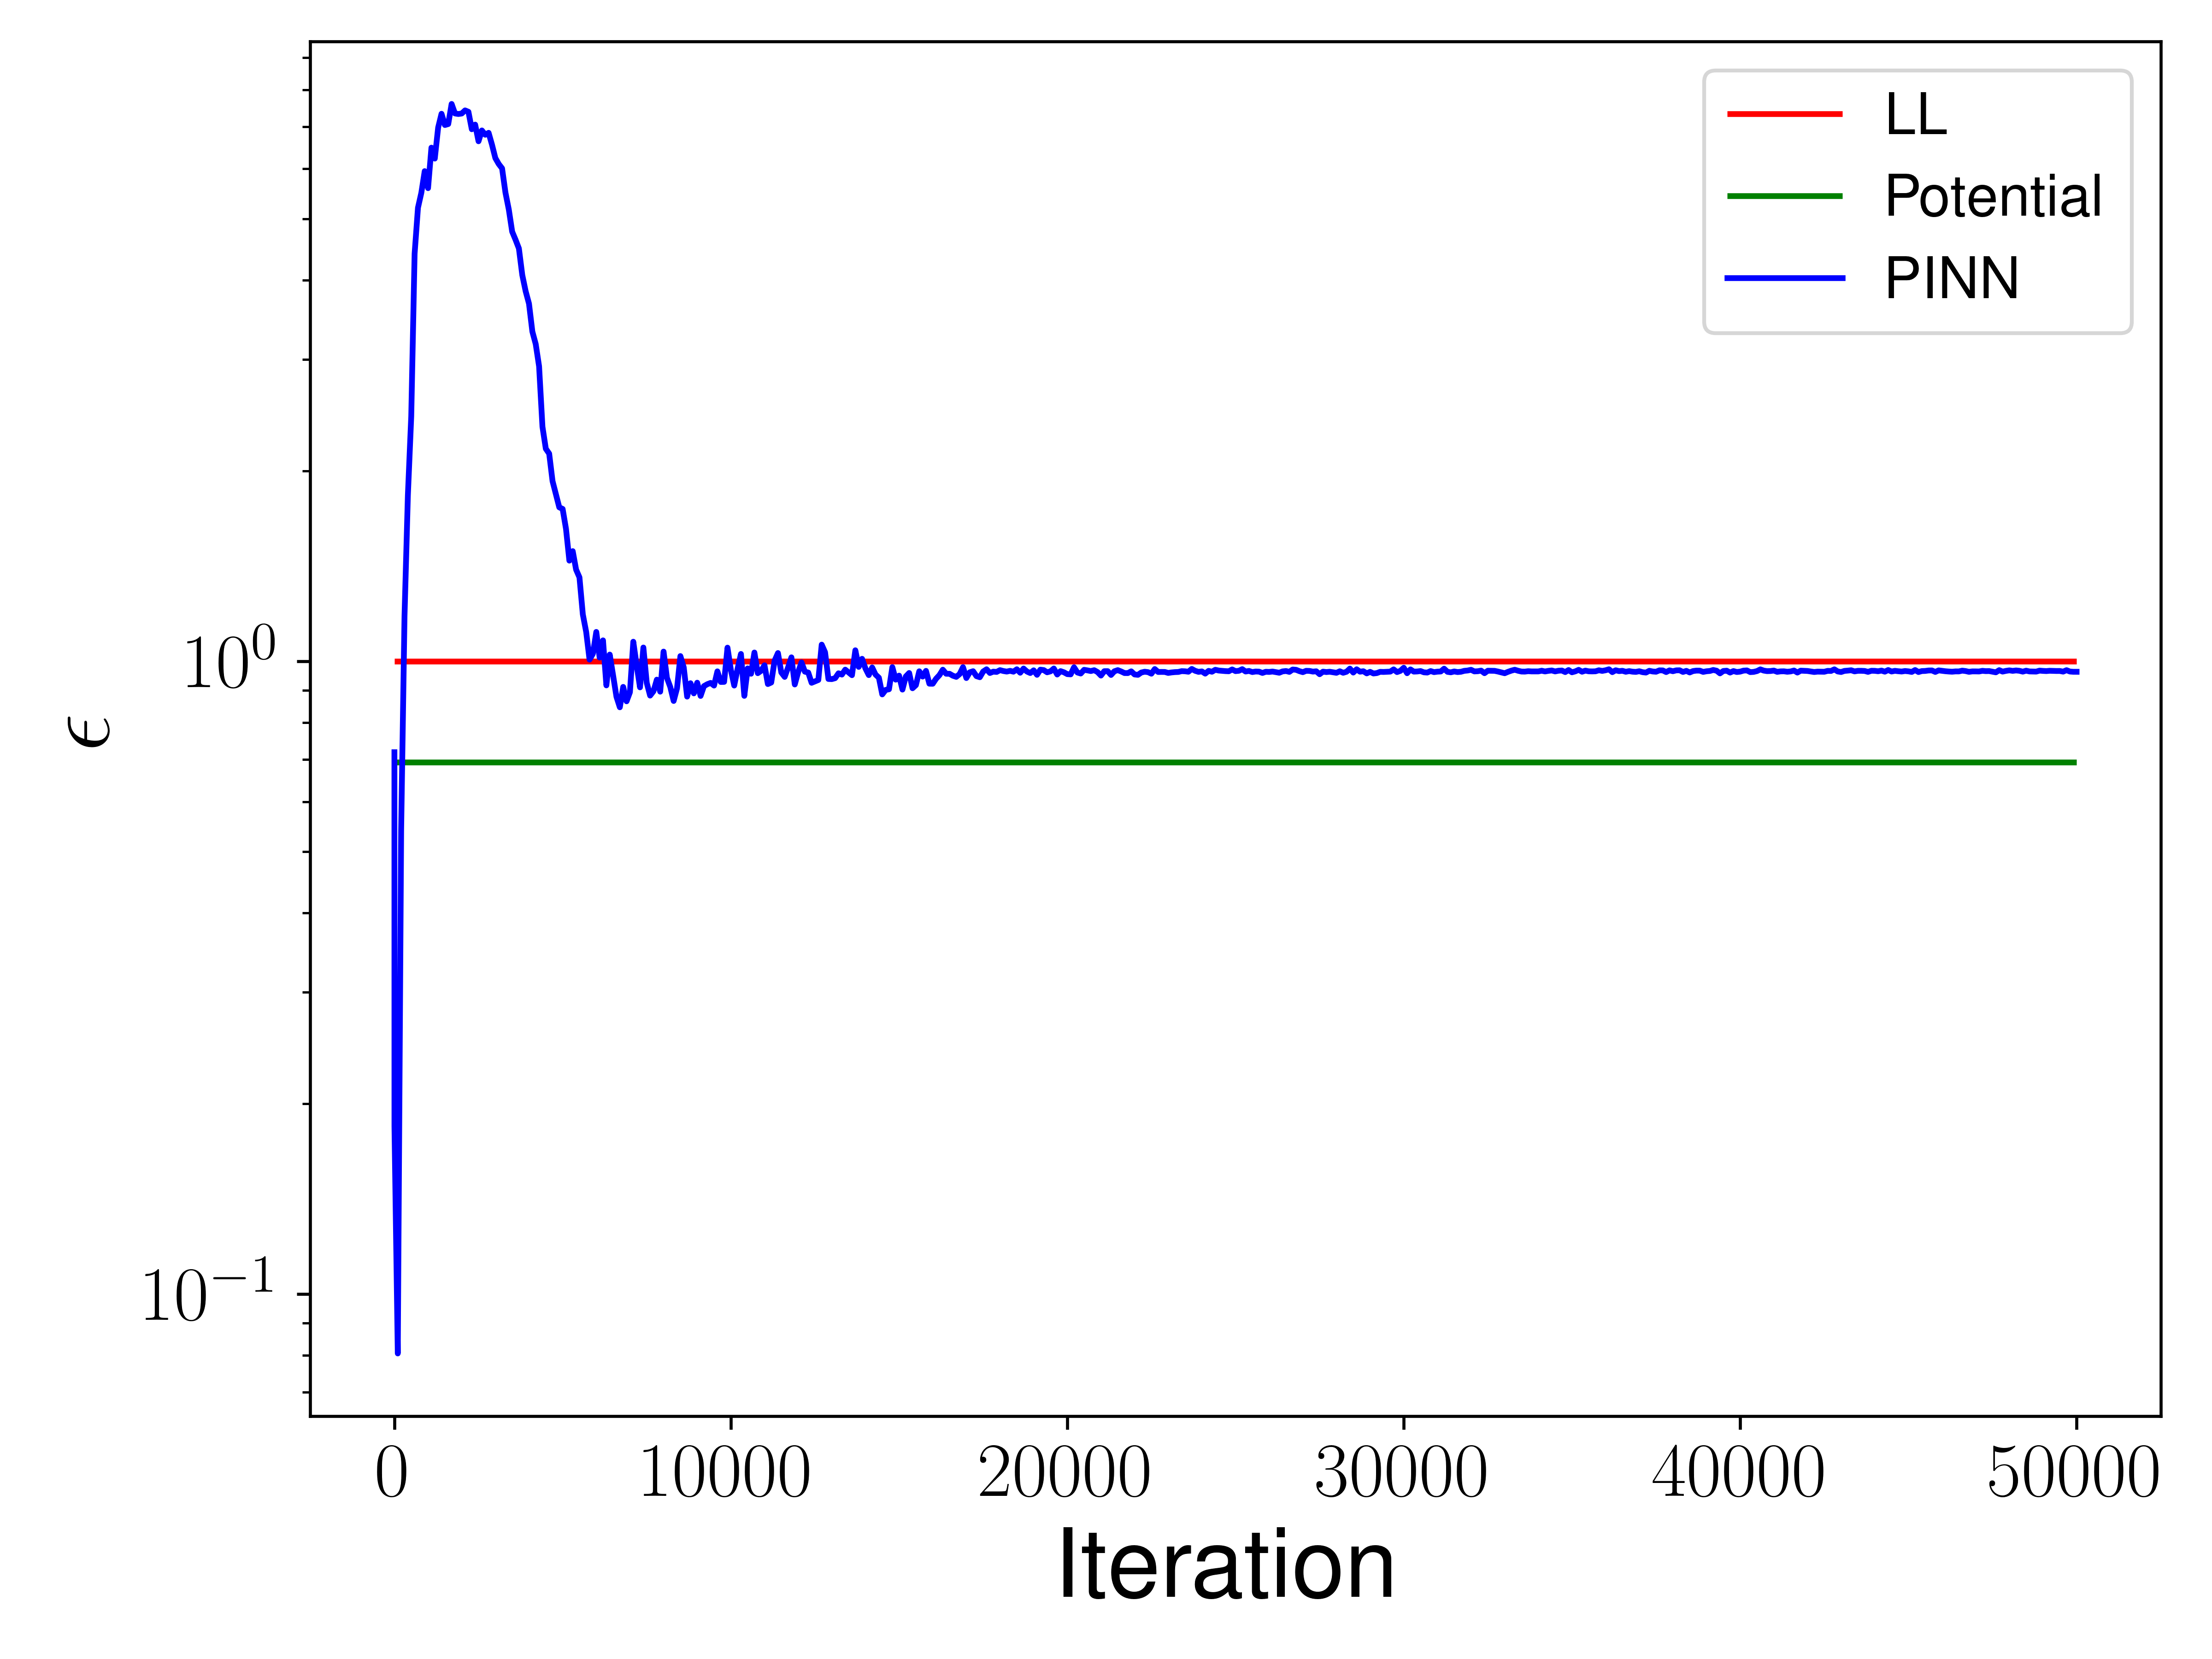
\includegraphics[width=\linewidth]{"img/graph/epsilon_ylog.png"}
    % \caption{The weighted loss of the force-free condition.}
  \end{subfigure}%
  \begin{subfigure}{.5\linewidth}
    \centering
    \caption{$\epsilon_p$}
    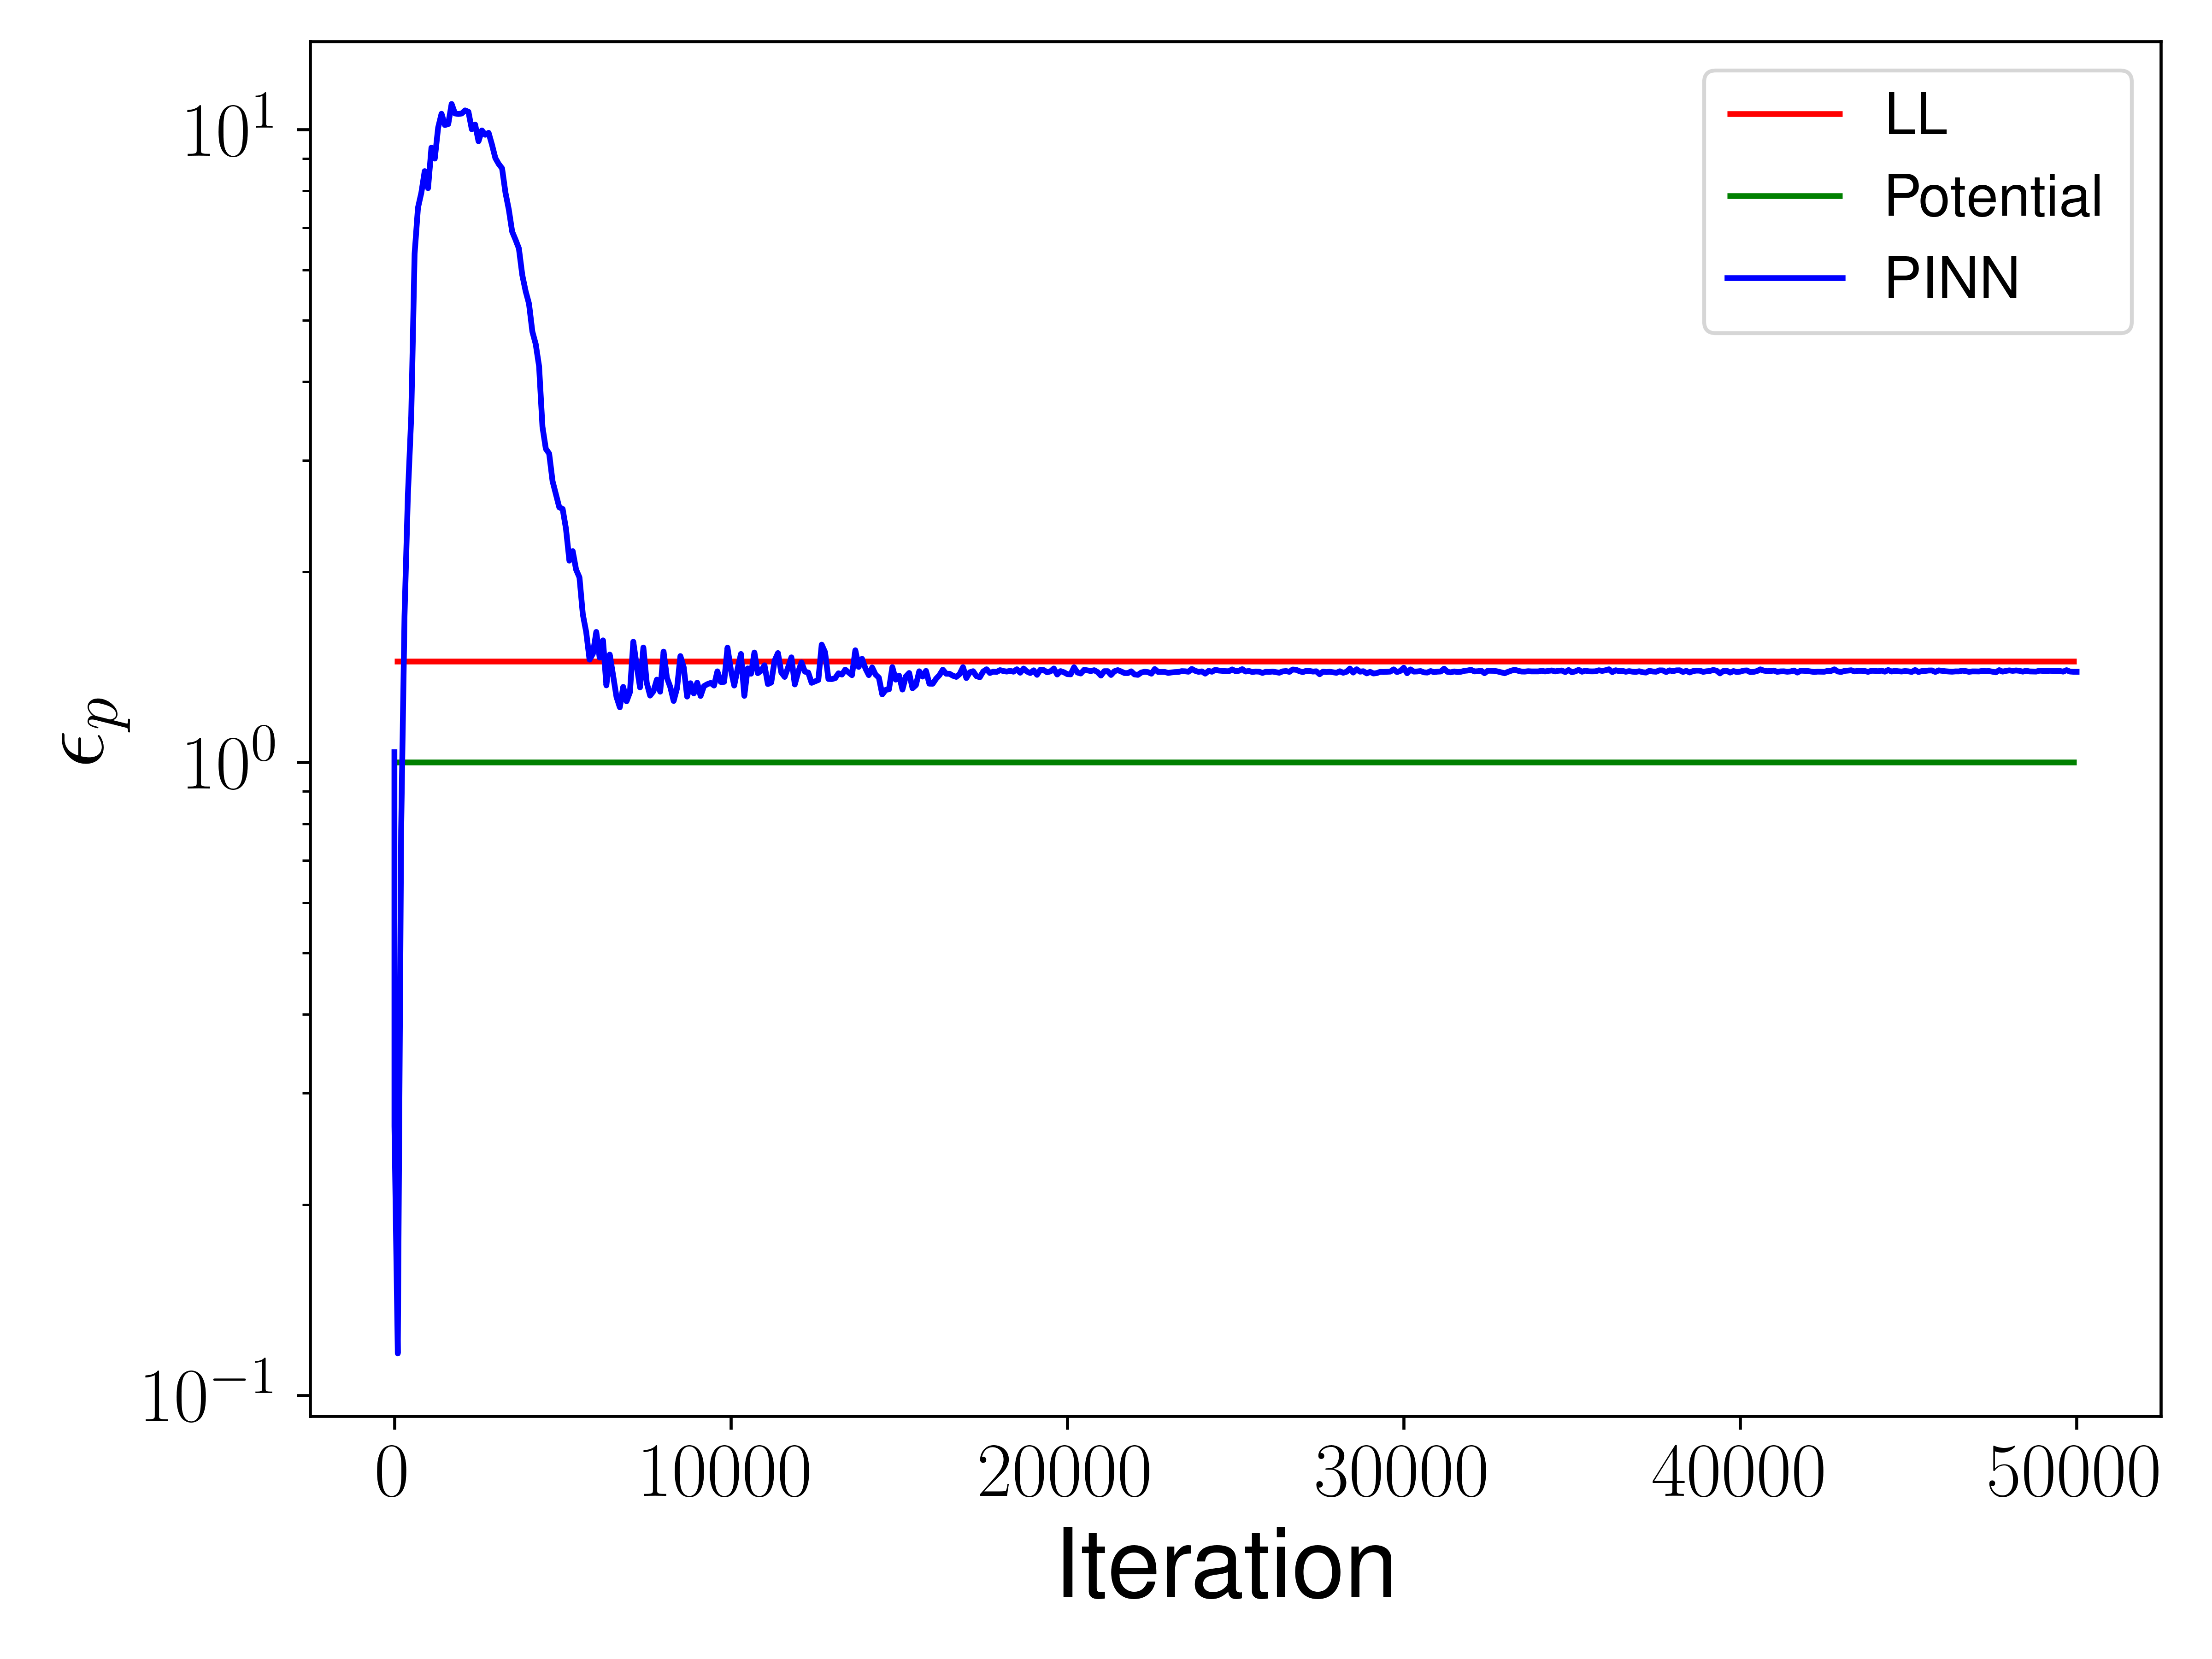
\includegraphics[width=\linewidth]{"img/graph/epsilon_p_ylog.png"}
    % \caption{The weighted loss of the solenoidal condition.}
  \end{subfigure}

  \begin{subfigure}{.5\linewidth}
    \centering
    \caption{$\text{CW}_\text{sin}$}
    \includegraphics[width=\linewidth]{"img/graph/CW_{text{sin}}.png"}
    % \caption{The weighted loss of the force-free condition.}
  \end{subfigure}%
  \begin{subfigure}{.5\linewidth}
    \centering
    \caption{$\mathcal{L}$}
    \includegraphics[width=\linewidth]{"img/graph/mathcal{L}_ylog.png"}
    % \caption{The weighted loss of the solenoidal condition.}
  \end{subfigure}

  \caption{The figures of metrit and total loss of PINN with respect to the iteration steps. The red denotes Low-Lou (LL) model, the green denotes the potential field calulated using that LL model, and the blue denotes the magnetic field reconstructed by PINN. The y-axes of the graphs for $\epsilon$, $\epsilon_p$, and $\mathcal{L}$ are in a base-10 logarithmic scale.}\label{fig:metric}
\end{figure}

In the expressions of the figures of merit, the variable $i$ represents each individual point within the computational domain, $M$ corresponds to the total number of points in the computational domain, $\mathbf{B}_{\text{p}}$ is the potential magnetic field whose bottom boundary condition is the same as that of $\mathbf{B}$, and $\mathbf{J} = \nabla \times \mathbf{B}$ is the current density in an appropriate unit system. The vector correlation metric $C_\text{vec}$ serves as a correlation coefficient specifically designed for vector fields. It has a value of $1$ when the vectors $\mathbf{B}$ and $\mathbf{b}$ are identical, and $0$ when $\mathbf{B}_i$ is perpendicular to $\mathbf{b}_i$ at each point. The Cauchy-Schwartz metric $C_\text{CS}$ quantifies the angles between vector fields. For $\mathbf{B}$ and $\mathbf{b}$ that are parallel, $C_\text{CS}$ equals $1$, while it becomes $-1$ for an anti-parallel case. When $\mathbf{B}_i$ is perpendicular to $\mathbf{b}_i$ at each point, $C_\text{CS}$ has a value of $0$. To measure the disparities between vector fields, the normalized and mean vector error metrics, $E_n$ and $E_m$ respectively, are employed. Both $E_n$ and $E_m$ are set to $0$ when $\mathbf{B}$ and $\mathbf{b}$ are identical. Since only these two metrics yield zero for a perfect match between $\mathbf{B}$ and $\mathbf{b}$, it is common to use $E'_n=1-E_n$ and $E'_m=1-E_m$ instead. Throughout this thesis, I have utilized $E'_n$ and $E'_m$. The total magnetic energy ratio, denoted as $\epsilon$, represents the ratio between the total magnetic energy of the two vector fields, $\mathbf{B}$ and $\mathbf{b}$. When $\mathbf{B}$ and $\mathbf{b}$ are identical, $\epsilon$ equals $1$.  Hence, if the physics-informed neural network method accurately reconstructs the Low-Lou analytical solution, all five metrics—$C_\text{vec}$, $C_\text{CS}$, $E'_n$, $E'_m$, and $\epsilon$—will be equal to $1$.

Considering that the potential field represents the state of lowest possible energy of any force-free fields with the same boundary condition, the magnetic energy of a nonlinear force-free field always surpasses that of the potential field. The surplus energy is known as free magnetic energy, which characterizes the energy associated with solar activities. The ratio $\epsilon_p$ between the total magnetic energy and the potential field energy indicates the amount of free magnetic energy stored in the nonlinear force-free field. For any field other than the potential field, $\epsilon_p$ exceeds $1$. The current-weighted sine metric, denoted as $\text{CW}_\text{sin}$, serves as an indicator of the force-freeness of the calculated magnetic field $\mathbf{B}$. When $\mathbf{B}$ is an exact force-free field, $\text{CW}_\text{sin}$ equals $0$. However, this metric, $\text{CW}_\text{sin}$, cannot be defined for the potential field because it has zero current density, $\mathbf{J}=\mathbf{0}$.

%For an alternative metric, I used the ratio $\zeta$ of the magnitude of the current density,
% \begin{equation*}
%   \zeta = \frac{\sum_i |\mathbf{J}_i|}{\sum_i |\mathbf{j}_i|},
% \end{equation*}
% where $\mathbf{J} = \nabla \times \mathbf{B}$ and $\mathbf{j} = \nabla \times \mathbf{b}$: $\zeta=1$ when the fields $\mathbf{B}$ and $\mathbf{b}$ are identical, $\zeta=0$ when the field $\mathbf{B}$ is a potential field, and  $\zeta$ is small when the field $\mathbf{B}$ has small free magnetic energy compared to the reference field $\mathbf{b}$, i.e., it is similar to the metric $\epsilon_p$ but it does not use the potential field to calculate the metric.

The optimizer of PINN aims to minimize the loss function $\mathcal{L}$ in a 528,131-dimensional parameter space. As a result, the loss function of PINN does not typically exhibit a monotonic decrease with respect to the iteration steps, as shown in \cref{fig:loss}. Although all the losses generally exhibit a monotonically decreasing trend after reaching certain critical points, the presence of numerous spikes in the graph indicates the challenges posed by the high-dimensionality of the parameter space. Initially, due to the high value of the boundary condition weight $w_b$ (starting from 1000), the weighted boundary condition loss $w_b\mathcal{L}_b$ dominates the total loss. Subsequently, as the boundary condition weight $w_b$ exponentially decreases, the weighted PDE losses $w_\text{ff}\mathcal{L}_\text{ff}$ and $w_\text{div}\mathcal{L}_\text{div}$ become increasingly influential in the total loss. In that time, they already has the decreasing pattern like the BC loss. Therefore, the overall pattern of the total loss closely resembles that of the boundary condition loss. 

The force-free condition loss $\mathcal{L}_\text{ff}$ and the solenoidal condition loss $\mathcal{L}_\text{div}$ display patterns of both increase and decrease. This behavior can be attributed to the fact that the initial field generated randomly for PINN, in this case, is a nearly constant vector field, as depicted in (a) of \cref{fig:xy,fig:yz,fig:xz,fig:xz_tilted}. Consequently, the derivatives of the initial magnetic field are close to zero, resulting in nearly zero PDE losses $\mathcal{L}_\text{ff}$ and $\mathcal{L}_\text{div}$.

As the training progresses, the field reconstructed by PINN satisfies the boundary conditions at $\partial V$, but it may not adhere to the force-free condition and solenoidal condition due to the initially high boundary condition weight $w_b$. Once the weighted boundary condition loss decreases sufficiently, the optimizer focuses on minimizing the PDE losses within the volume $V$, which now constitute the majority of the total loss. Consequently, the field gradually evolves into a nonlinear force-free field that satisfies the prescribed boundary conditions while simultaneously reducing the PDE losses. 

Although the primary objective of the optimizer is to minimize the total loss $\mathcal{L}$, the seven metrics ($C_\text{vec}$, $C_\text{CS}$, $E'_n$, $E'_m$, $\epsilon$, $\epsilon_p$, and $\text{CW}_\text{sin}$) of the PINN-reconstructed magnetic field closely resemble those of the Low-Lou model, as depicted in \cref{fig:metric}. This observation confirms that the loss function employed in traditional optimization methods can also be utilized in the PINN approach, demonstrating the ability of the physics-informed neural network method to reconstruct nonlinear force-free fields. It is worth noting that the PINN-reconstructed solution surpasses the potential field as it exhibits closer proximity to the Low-Lou analytical solution.

However, while $\mathcal{L}$ serves as a valuable loss function, it is not flawless. As shown in \cref{tab:metric}, the figures of merit ($C_\text{vec}$, $E'_n$, $E'_m$, $\epsilon$, and $\epsilon_p$) for the PINN(50000) model are inferior (deviating from the values of the Low-Lou model) compared to those of the PINN(25000) model, even though $\mathcal{L}$ decreases from 0.00006 to 0.00005. Meanwhile, $C_\text{CS}$ and $\text{CW}_\text{sin}$ for the PINN(50000) model outperform those of the PINN(25000) model. This observation suggests the need for the development of more appropriate loss functions in future research.

Furthermore, the energy metrics $\epsilon$ and $\epsilon_p$ of the PINN(50000) model exhibit lower values compared to the Low-Lou solution. This indicates that the total magnetic energy and free magnetic energy of the PINN(50000) model are smaller than those of the Low-Lou solution. This finding may imply the presence of spectral bias in the PINN method \parencite{rahaman2019spectral}, i.e., the neural network tends to prioritize learning low-frequency features while facing challenges with high-frequency features. Actually, a smooth distribution of magnetic fields, favored by the PINN approach, typically results in lower magnetic energy compared to a more spiky distribution because of the squaring operation in the definition of magnetic energy $\int_{V} \frac{B^2}{8\pi} \mathrm{d}V$: $8 = 2^2 + 2^2 < 3^2 + 1^2 = 10$.

The colors in the $z=0$ plane in the \cref{fig:xy,fig:yz,fig:xz,fig:xz_tilted} follows the typical convention for solar magnetograms: white represents positive $B_z$ values, while black represents negative $B_z$ values. All figures share the same scalar bar, which spans a range of (-150, 150). Additionally, 25 field lines have been selected, and each field line is assigned a unique color to distinguish it from the others. The colors are randomly assigned based on the seed value calculated from the coordinates of the field line's starting point. Thus, the field lines originating from the same point have the same color across all figures. These figures demonstrate that the PINN method successfully reconstructs the nonlinear force-free fields described by the Low-Lou model in qualitative terms. Furthermore, PINN(0) in these figures highlight that PINN does not require any pre-calculated initial field, such as a potential field, as is typically needed in traditional optimization methods.

\begin{table*}
  \centering
  \caption{Figures of merit for various fields and total loss of PINN. The reference field is the Low-Lou model with $(n=1, m=1, l=0.3, \Phi=\pi/2)$. PINN($i$) refers to the magnetic field calculated using PINN at the iteration step $i$.}\label{tab:metric}
  \begin{NiceTabular}{ccccccccc}
  \toprule
  Field & $C_\text{vec}$ & $C_\text{CS}$ & $E'_n$ & $E'_m$ & $\epsilon$ & $\epsilon_p$ & $\text{CW}_\text{sin}$ & $\mathcal{L}$\tabularnote{The total loss of PINN.} \\ 
  \midrule
  Low-Lou & 1.00000 & 1.00000 & 1.00000 & 1.00000 & 1.00000 & 1.44490 & 0.01308\tabularnote{This is not zero due to numerical grids.} & -- \\
  Potential & 0.86465 & 0.86925 & 0.43003 & 0.36242 & 0.69209 & 1.00000 & --\tabularnote{The metric $\text{CW}_\text{sin}$ is undefined for the potential field.} & -- \\
  PINN(0) & 0.07115 & 0.33540 & -1.37088 & -6.07067 & 0.71824 & 1.03779 & 0.55813 & 40.23570 \\
  PINN(100) & 0.25771 & 0.46100 & -0.00643 & -0.46701 & 0.08056 & 0.11640 & 0.76066 & 31.32017 \\
  PINN(1000) & 0.54244 & 0.32404 & -2.31914 & -6.41640 & 5.59377 & 8.08246 & 0.71701 & 6.46577 \\
  PINN(10000) & 0.98630 & 0.63065 & 0.68766 & 0.28275 & 0.96939 & 1.40068 & 0.38403 & 0.00848 \\
  PINN(25000) & 0.99402 & 0.92134 & 0.78452 & 0.55897 & 0.96481 & 1.39406 & 0.07853 & 0.00006 \\
  PINN(50000) & 0.99359 & 0.92271 & 0.77129 & 0.50928 & 0.96247 & 1.39068 & 0.06848 & 0.00005 \\
  \bottomrule
  \end{NiceTabular}
\end{table*}

\begin{figure}
  \begin{subfigure}{.5\linewidth}
    \centering
    \caption{$\mathcal{L}$}
    \includegraphics[width=\linewidth]{"img/graph/mathcal{L}_ylog.png"}
    % \caption{The total loss of PINN.}
  \end{subfigure}%
  \begin{subfigure}{.5\linewidth}
    \centering
    \caption{$w_b\mathcal{L}_b$}
    \includegraphics[width=\linewidth]{"img/graph/w_bmathcal{L}_b_ylog.png"}
    % \caption{The weighted loss of the boundary condition.}
  \end{subfigure}

  \begin{subfigure}{.5\linewidth}
    \centering
    \caption{$w_\text{ff}\mathcal{L}_\text{ff}$}
    \includegraphics[width=\linewidth]{"img/graph/w_text{ff}mathcal{L}_text{ff}_ylog.png"}
    % \caption{The weighted loss of the force-free condition.}
  \end{subfigure}%
  \begin{subfigure}{.5\linewidth}
    \centering
    \caption{$w_\text{div}\mathcal{L}_\text{div}$}
    \includegraphics[width=\linewidth]{"img/graph/w_text{div}mathcal{L}_text{div}_ylog.png"}
    % \caption{The weighted loss of the solenoidal condition.}
  \end{subfigure}

  \caption{The values of loss funtions with respect to the iteration steps. (a) The total loss of PINN. The weighted loss of (b) the boundary condition, (c) the force-free condition, and (d) the solenoidal condition. The y-axes of these graphs are in a base-10 logarithmic scale.}\label{fig:loss}
\end{figure}

\begin{figure}
  \begin{subfigure}{.5\linewidth}
    \centering
    \caption{PINN(0)}\label{fig:xy0}
    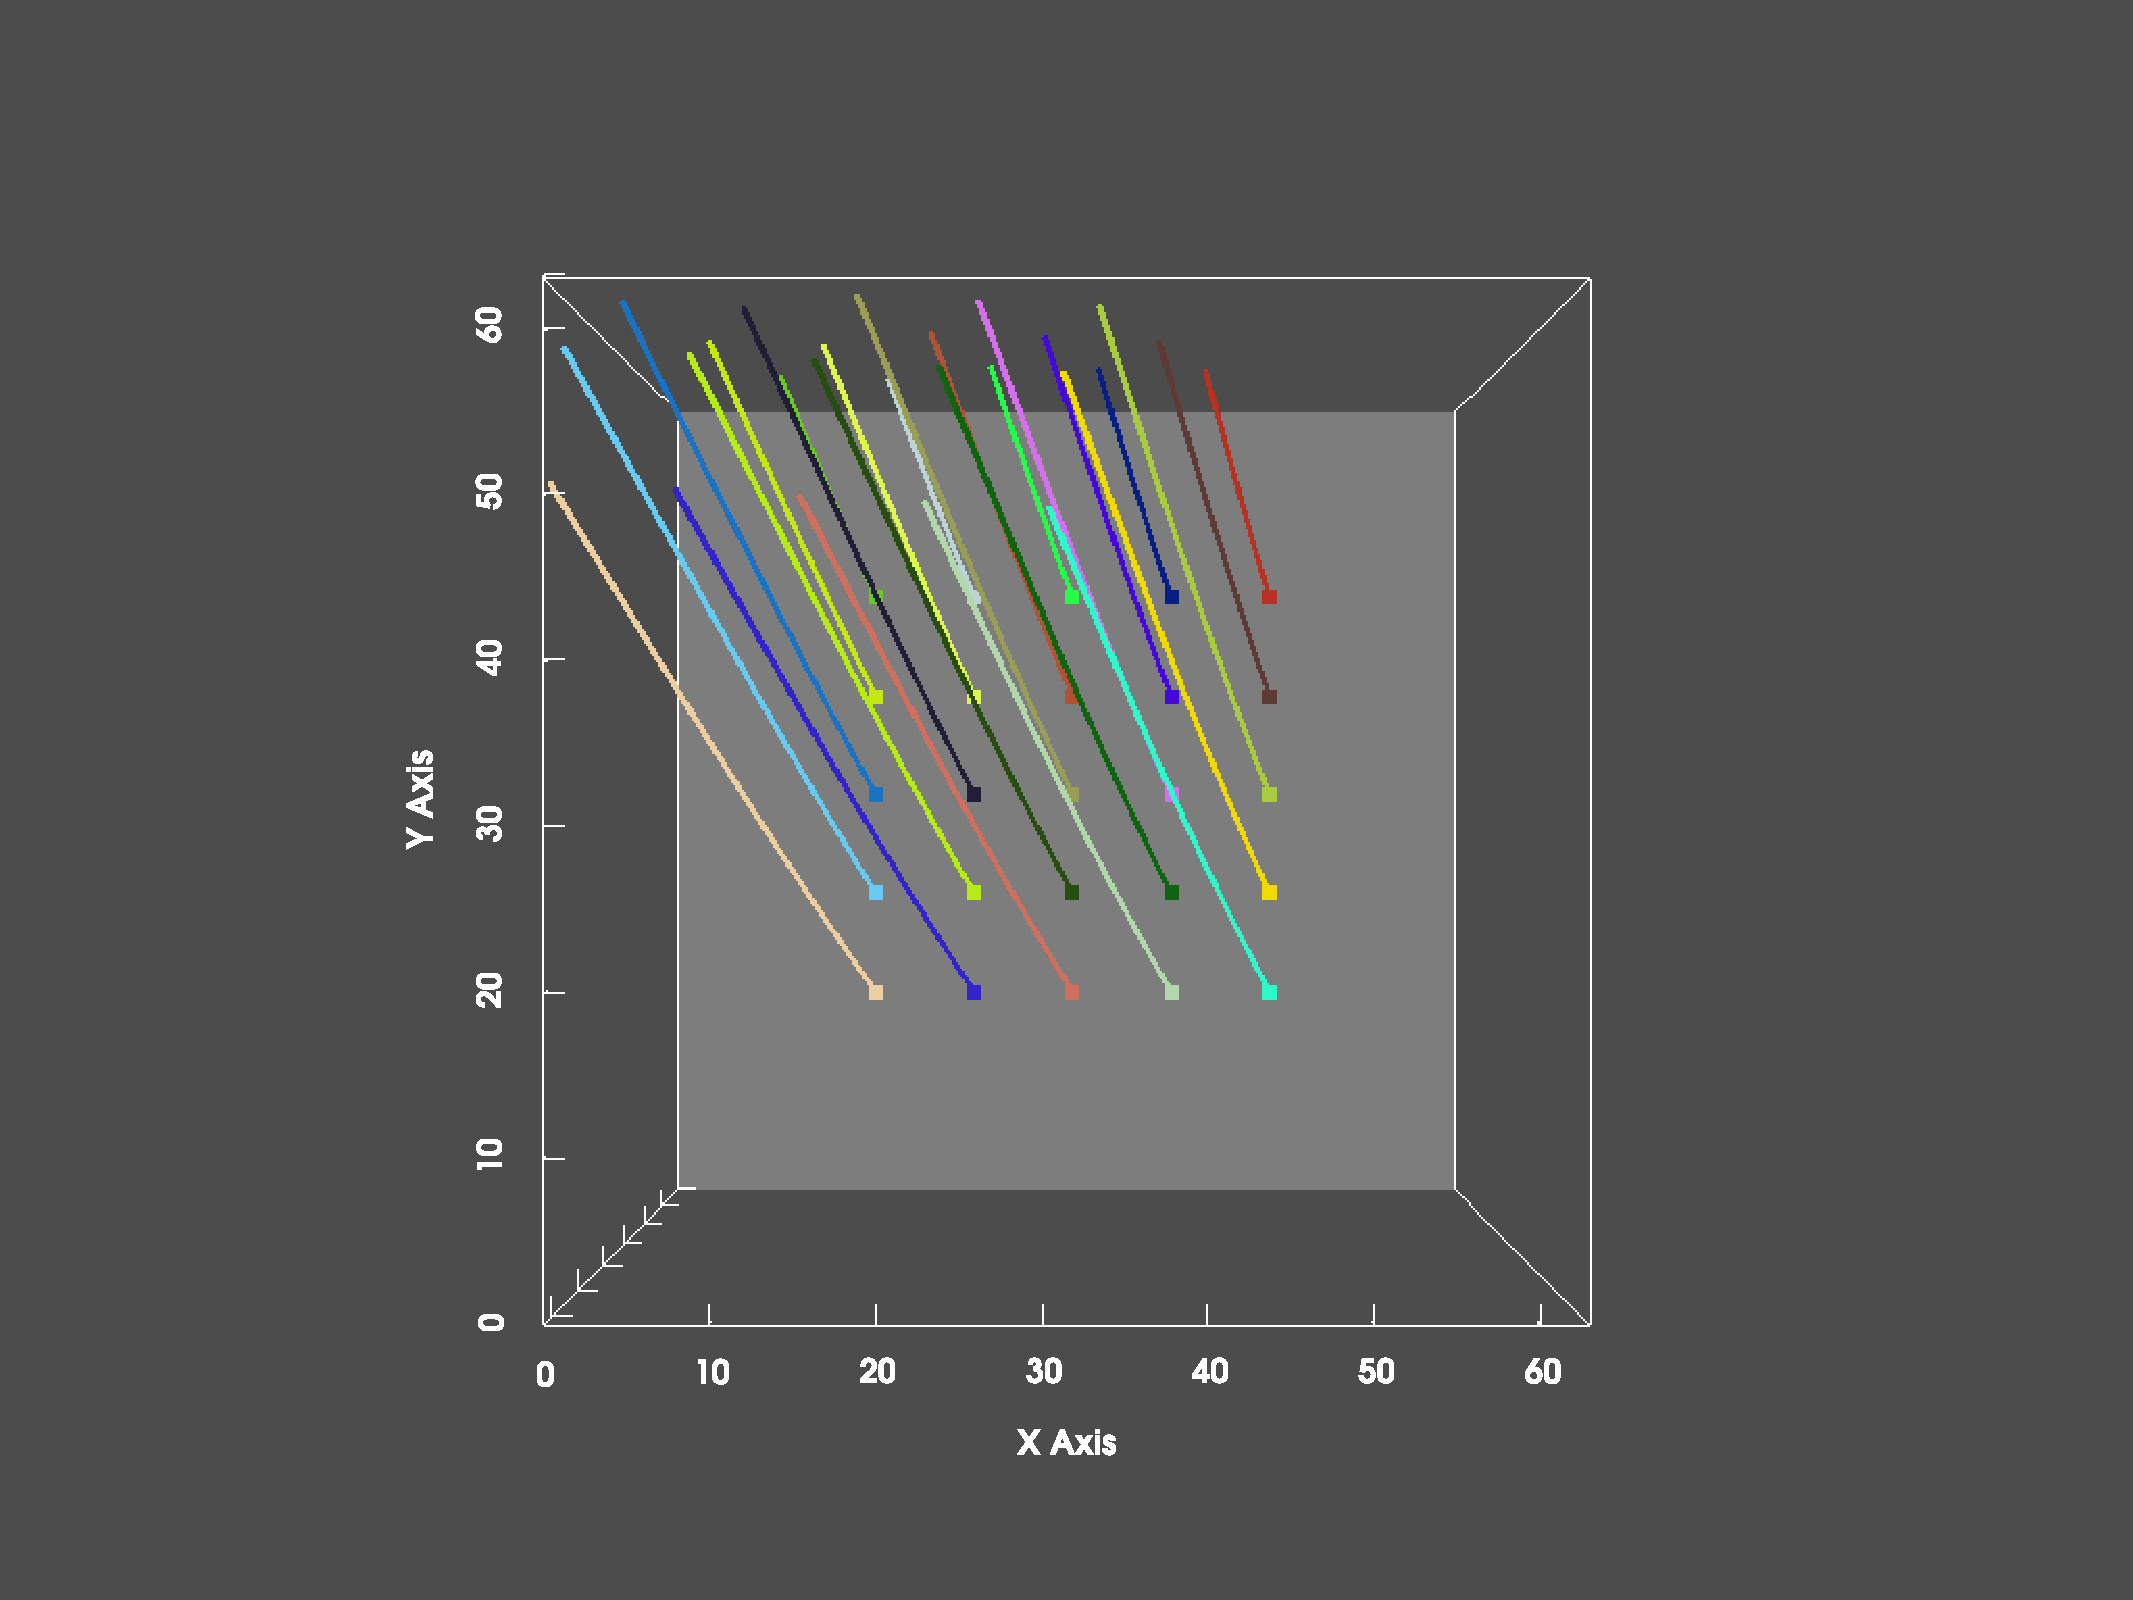
\includegraphics[trim={6cm 1cm 6cm 2cm}, clip, width=\linewidth]{"img/PINN_000000_xy.pdf"}
  \end{subfigure}%
  \begin{subfigure}{.5\linewidth}
    \centering
    \caption{PINN(100)}
    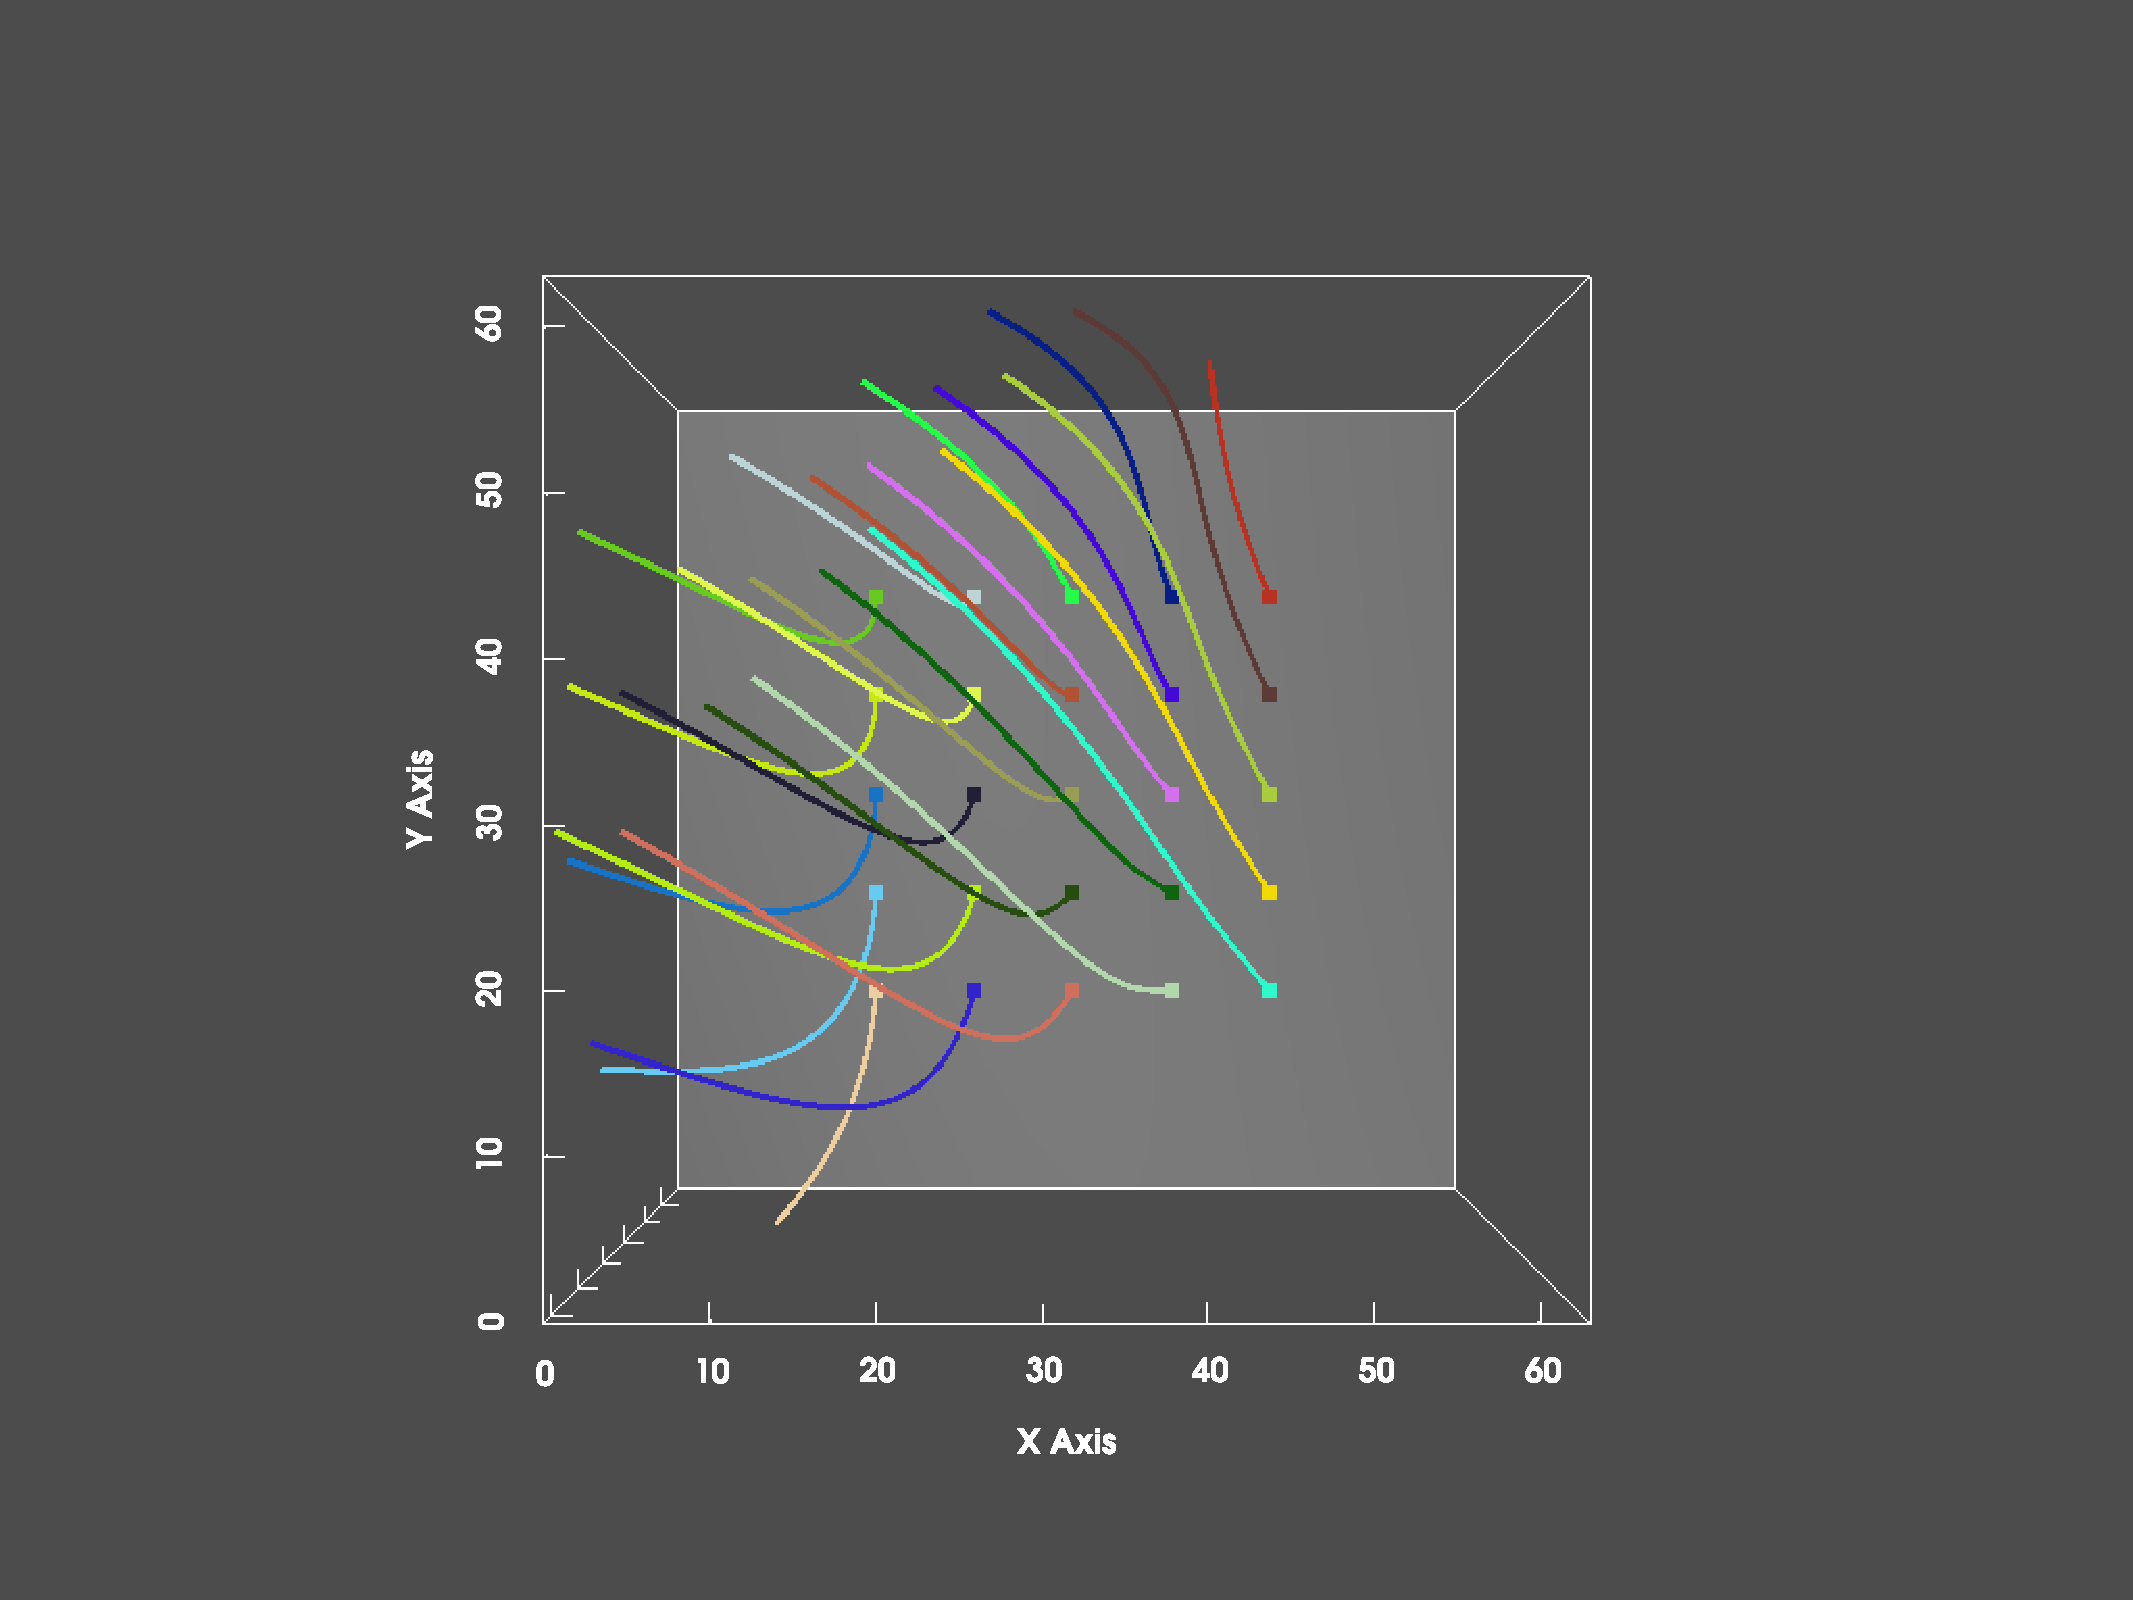
\includegraphics[trim={6cm 1cm 6cm 2cm}, clip, width=\linewidth]{"img/PINN_000100_xy.pdf"}
  \end{subfigure}

  \begin{subfigure}{.5\linewidth}
    \centering
    \caption{PINN(1000)}
    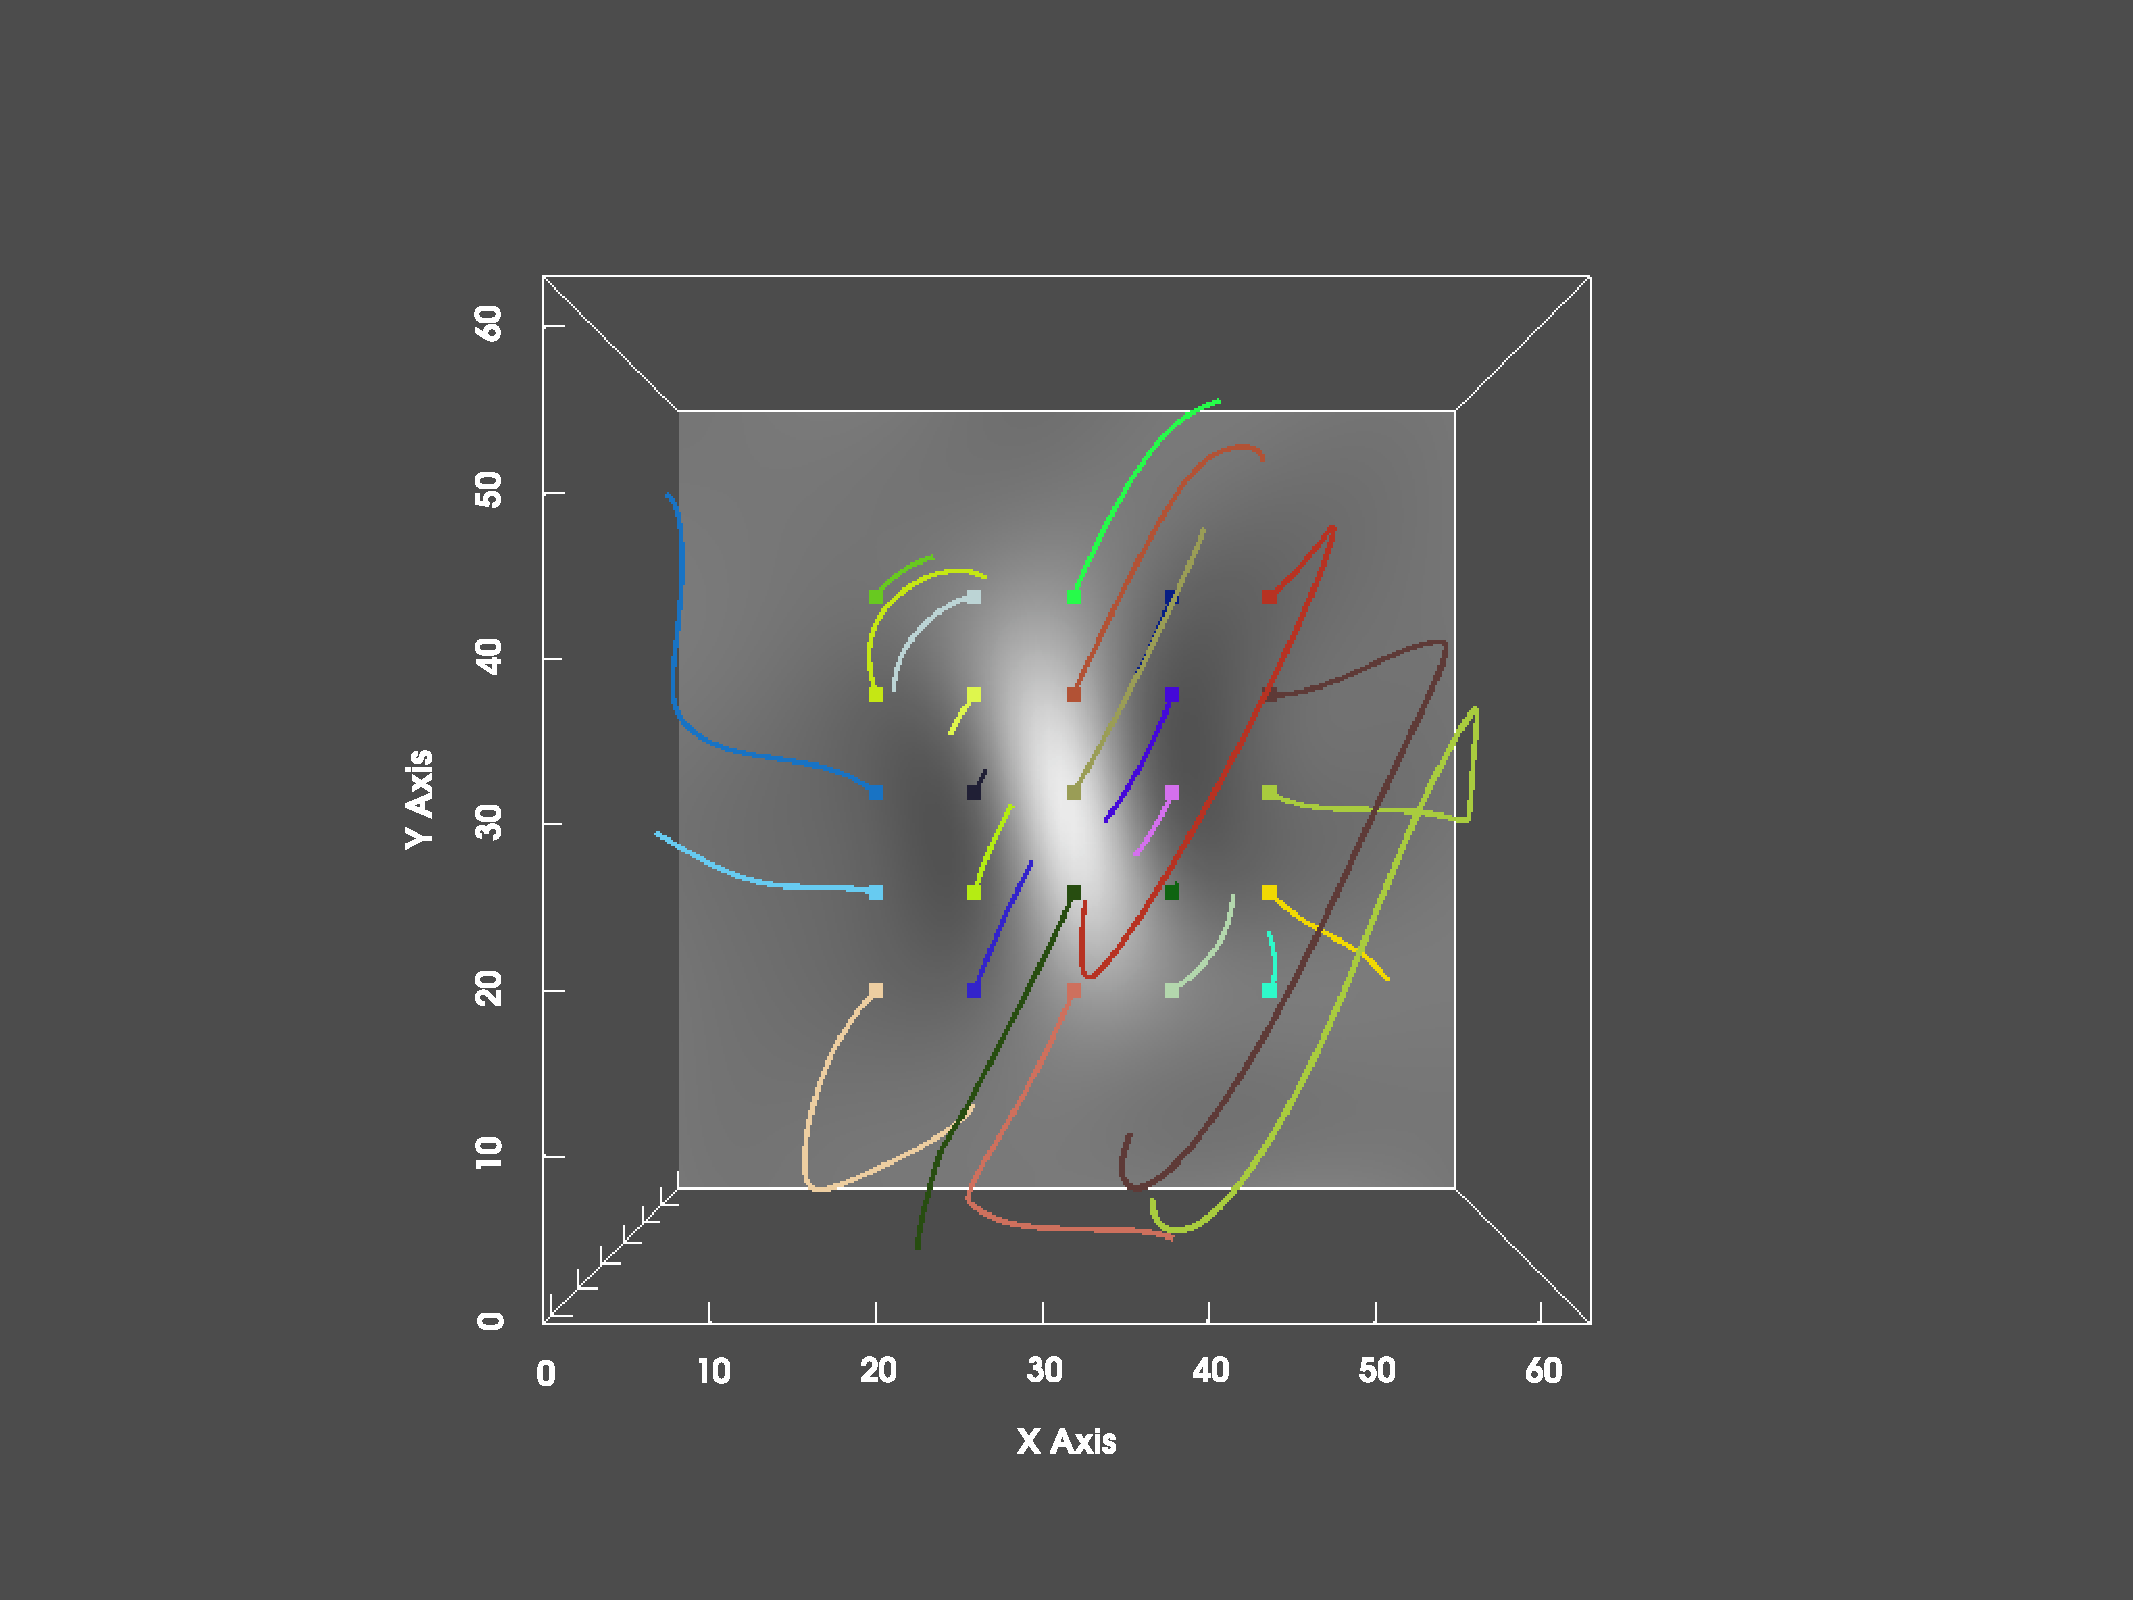
\includegraphics[trim={6cm 1cm 6cm 2cm}, clip, width=\linewidth]{"img/PINN_001000_xy.pdf"}
  \end{subfigure}%
  \begin{subfigure}{.5\linewidth}
    \centering
    \caption{PINN(10000)}
    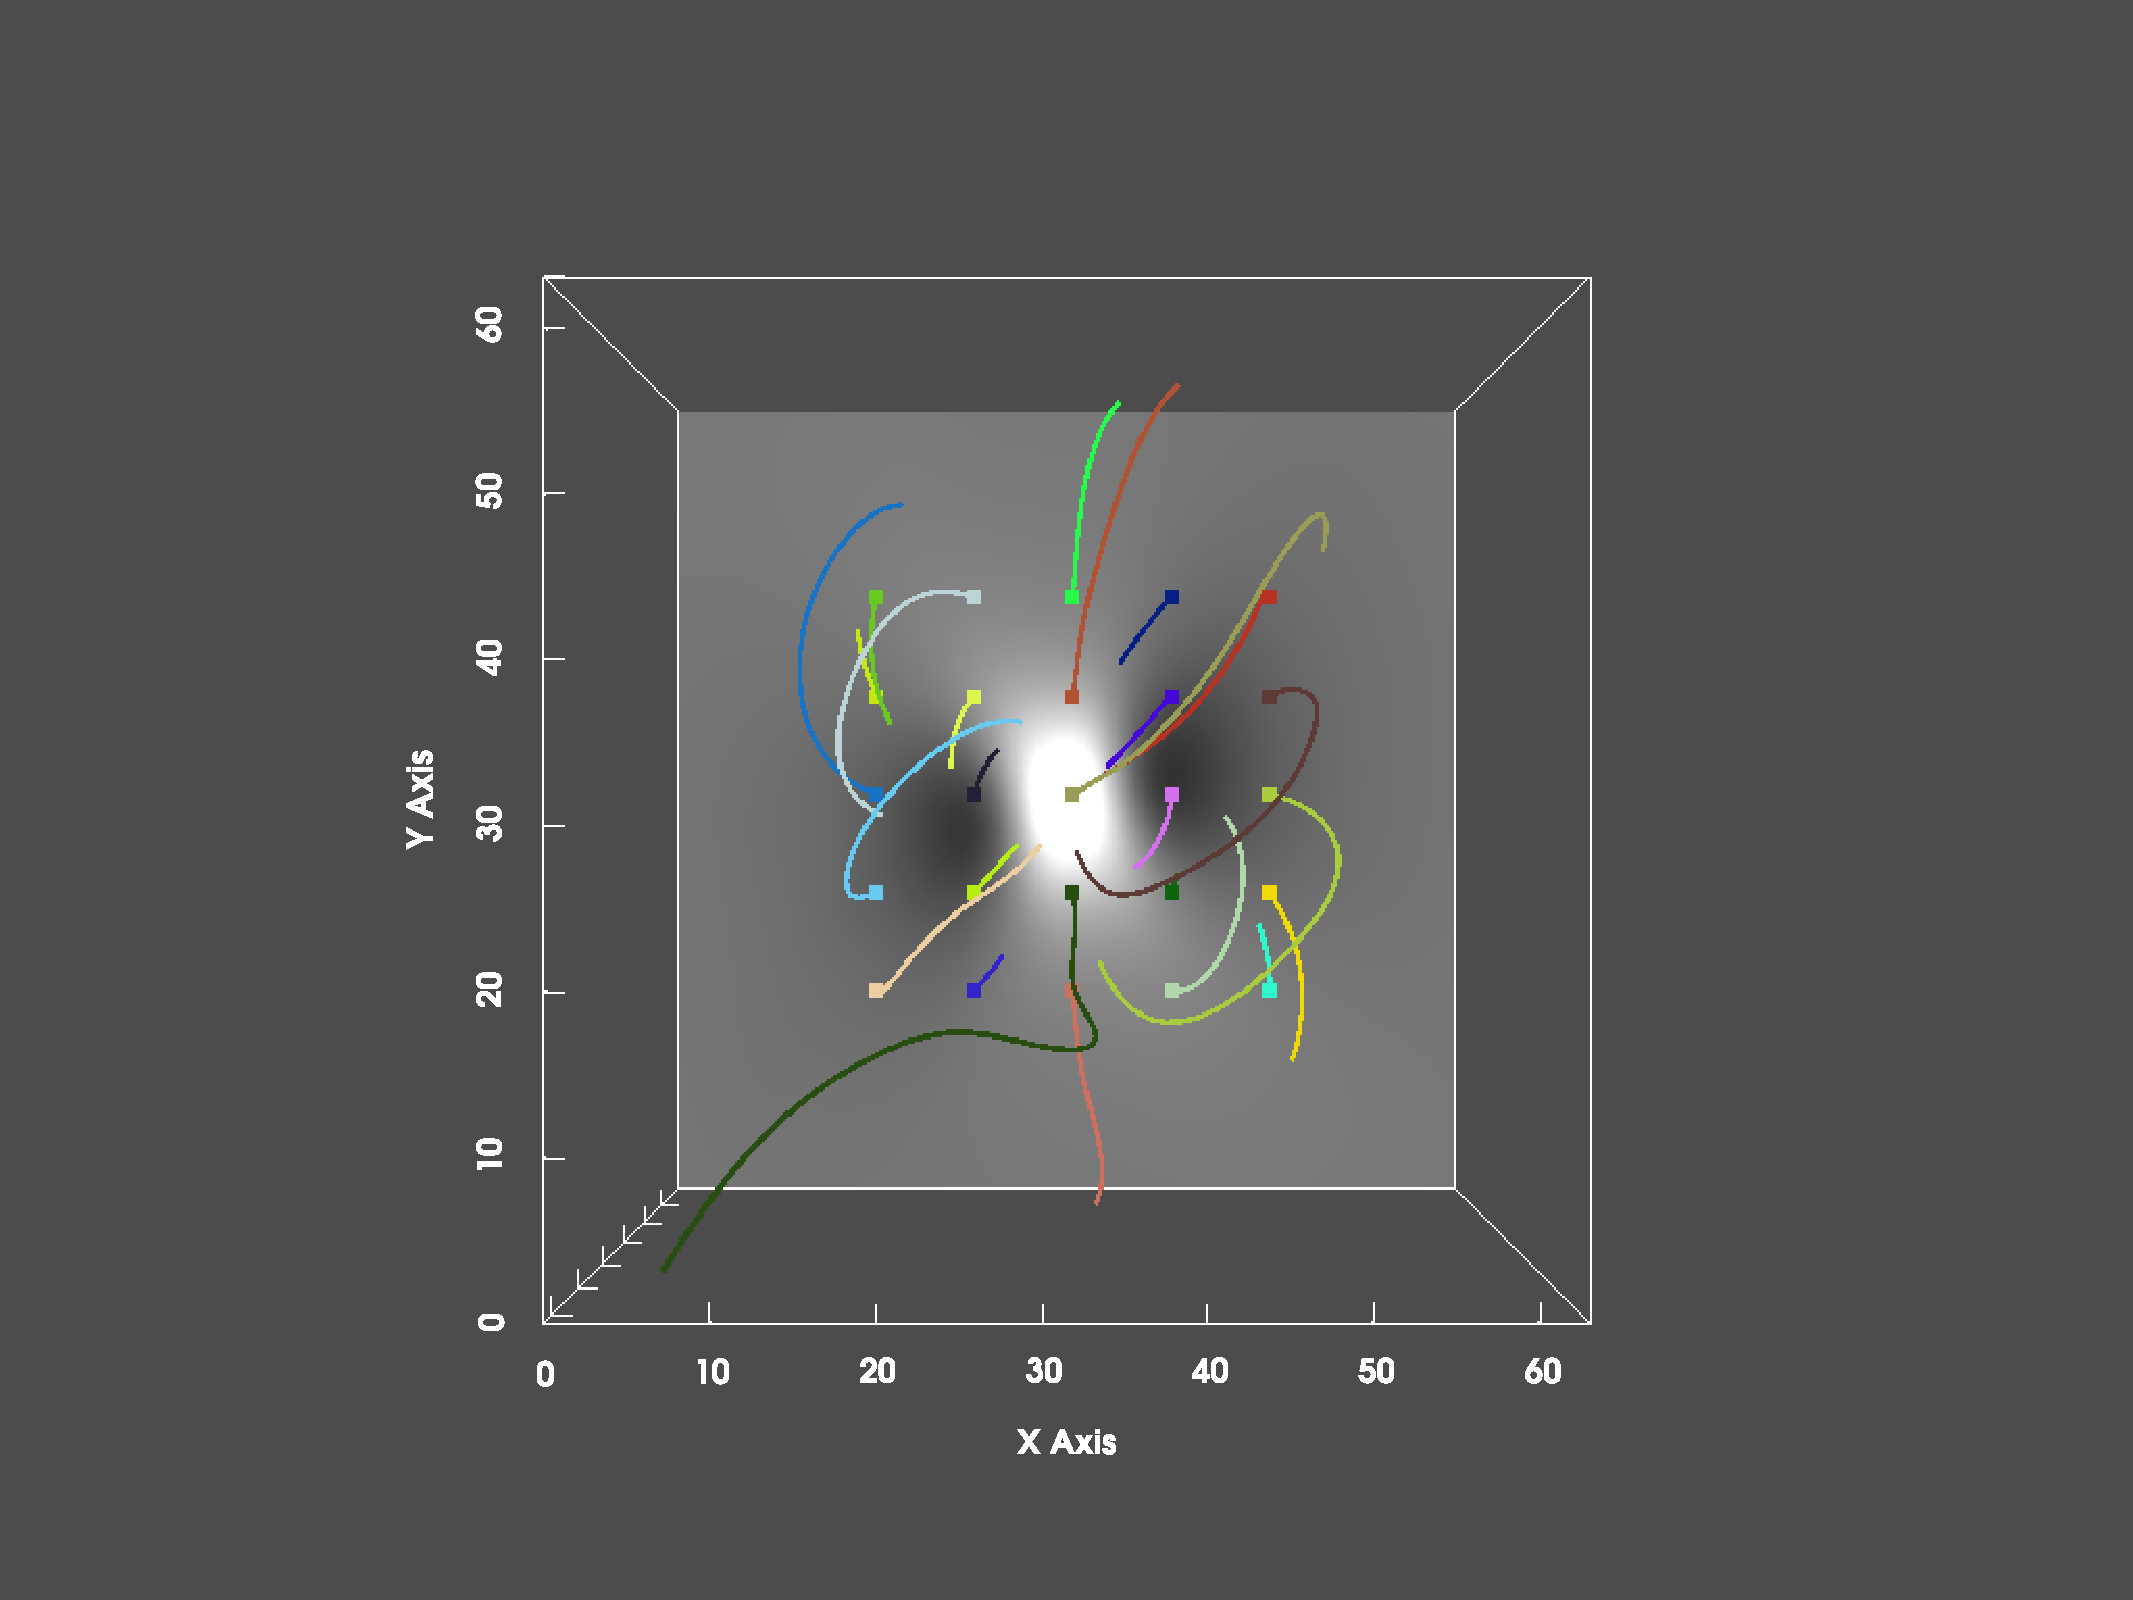
\includegraphics[trim={6cm 1cm 6cm 2cm}, clip, width=\linewidth]{"img/PINN_010000_xy.pdf"}
  \end{subfigure}

  \begin{subfigure}{.5\linewidth}
    \centering
    \caption{PINN(25000)}
    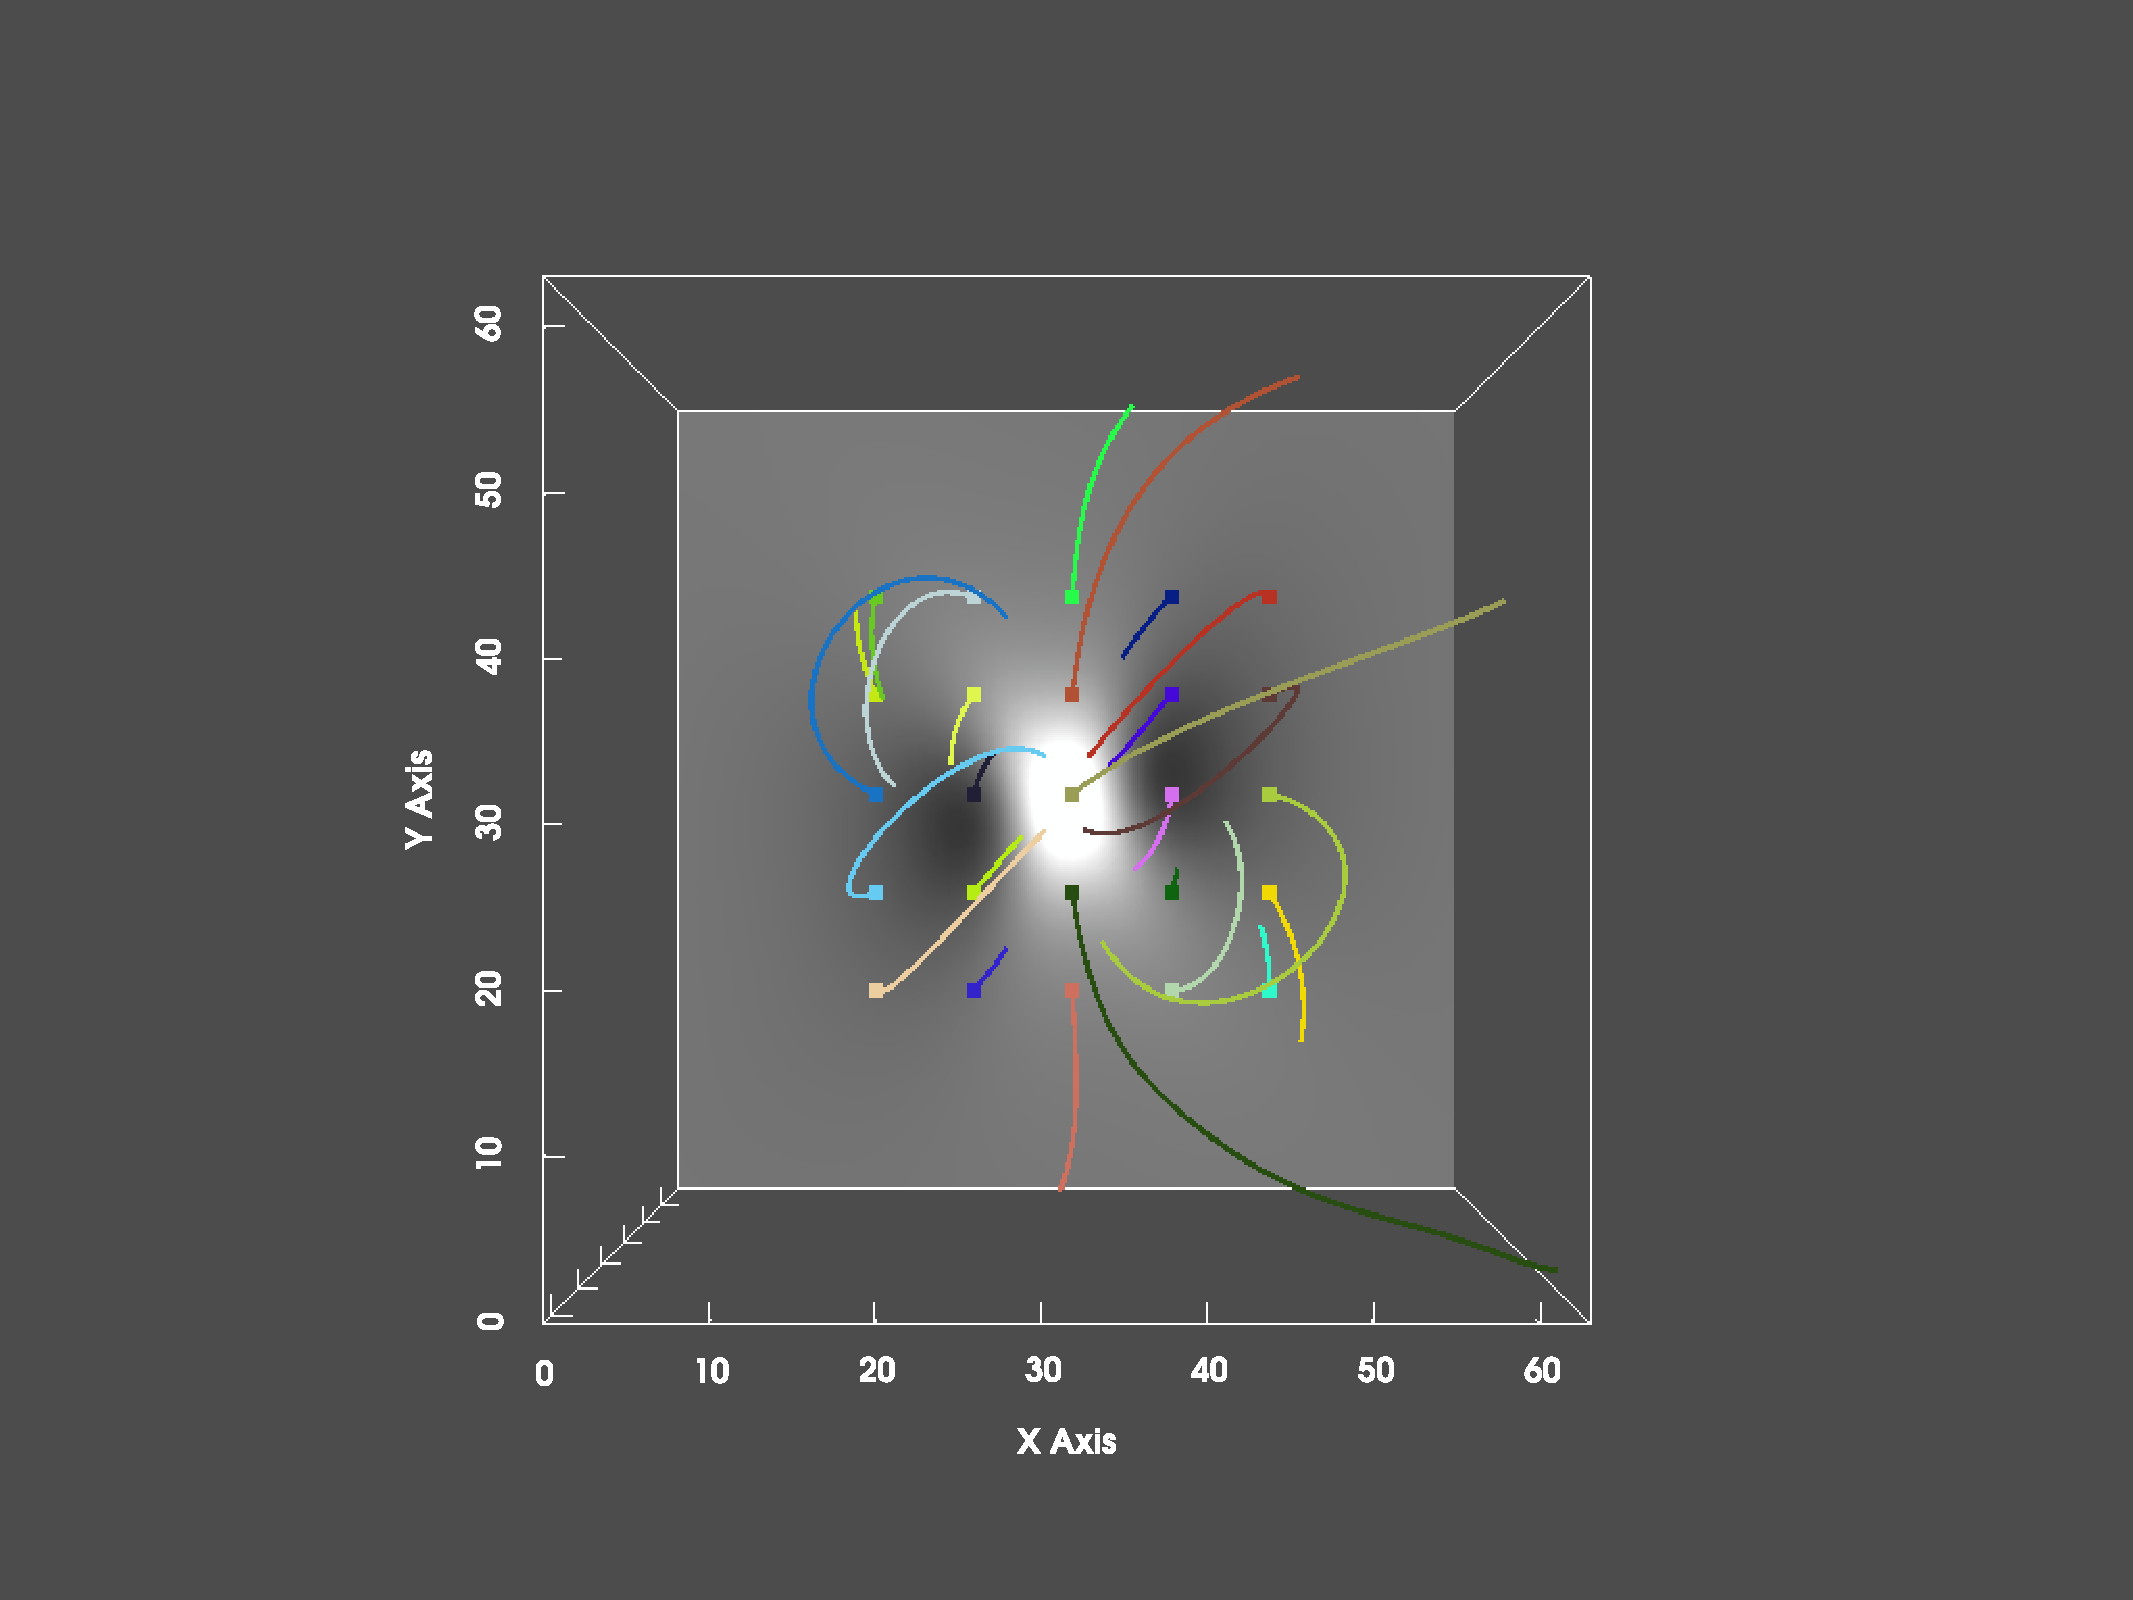
\includegraphics[trim={6cm 1cm 6cm 2cm}, clip, width=\linewidth]{"img/PINN_025000_xy.pdf"}
  \end{subfigure}%
  \begin{subfigure}{.5\linewidth}
    \centering
    \caption{PINN(50000)}
    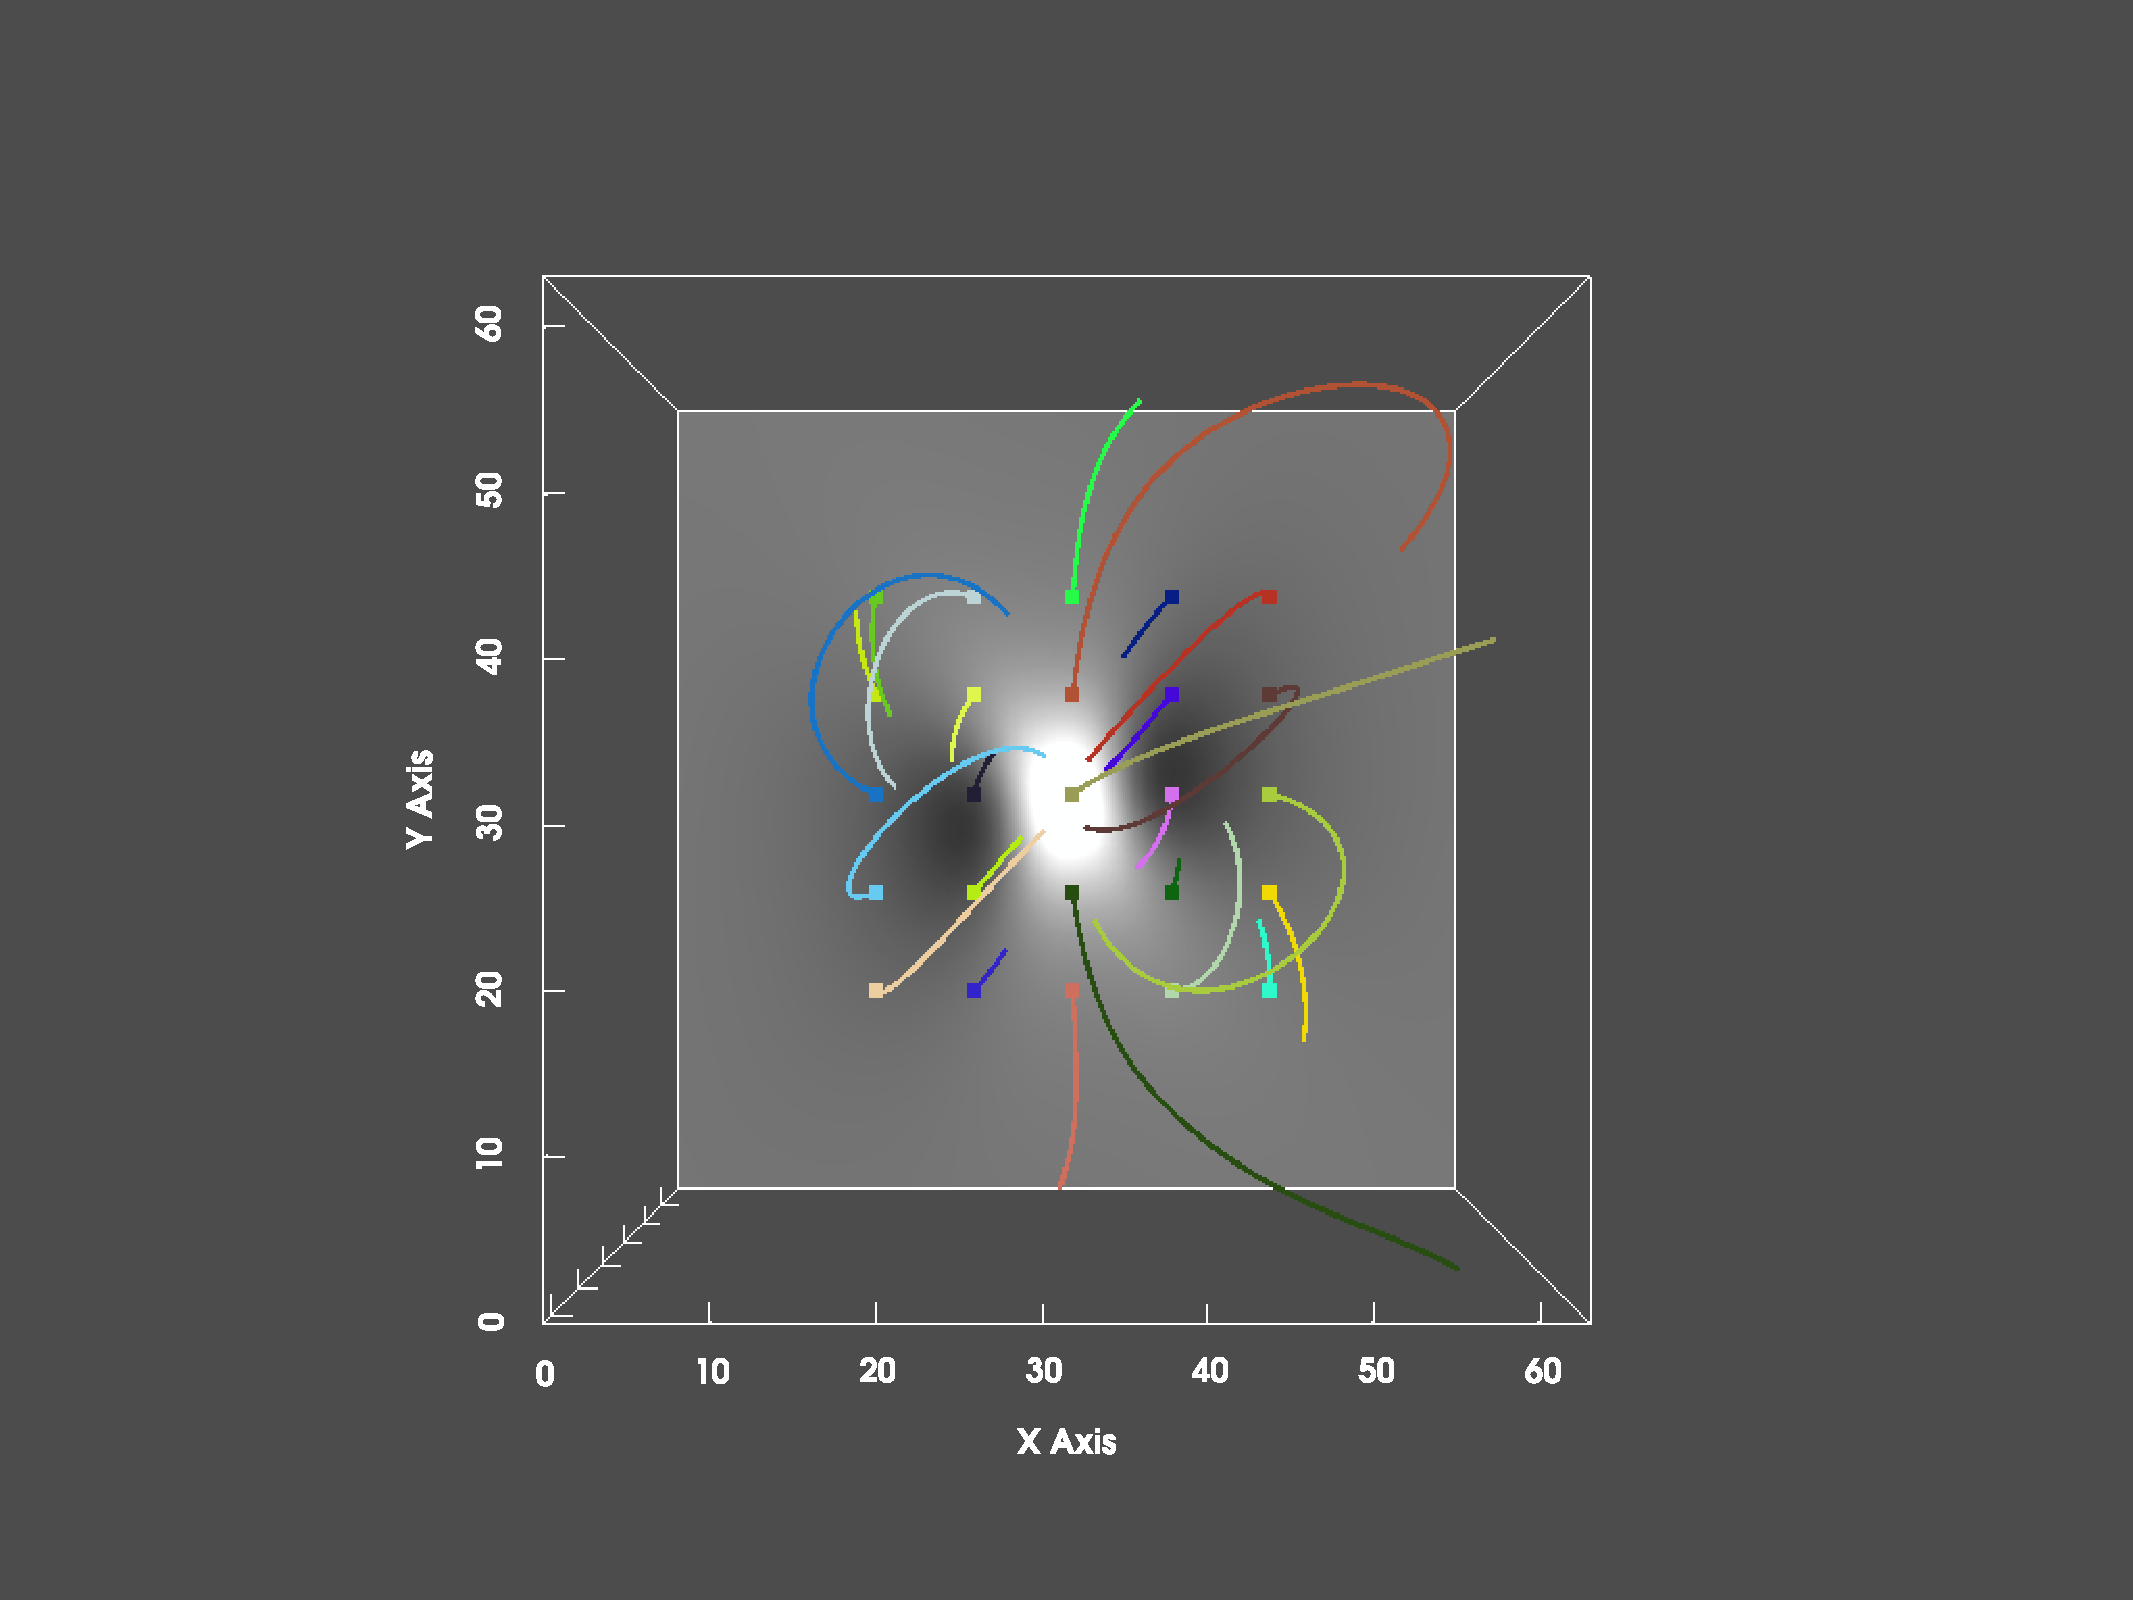
\includegraphics[trim={6cm 1cm 6cm 2cm}, clip, width=\linewidth]{"img/PINN_050000_xy.pdf"}
  \end{subfigure}
  
  \begin{subfigure}{.5\linewidth}
    \centering
    \caption{Potential}
    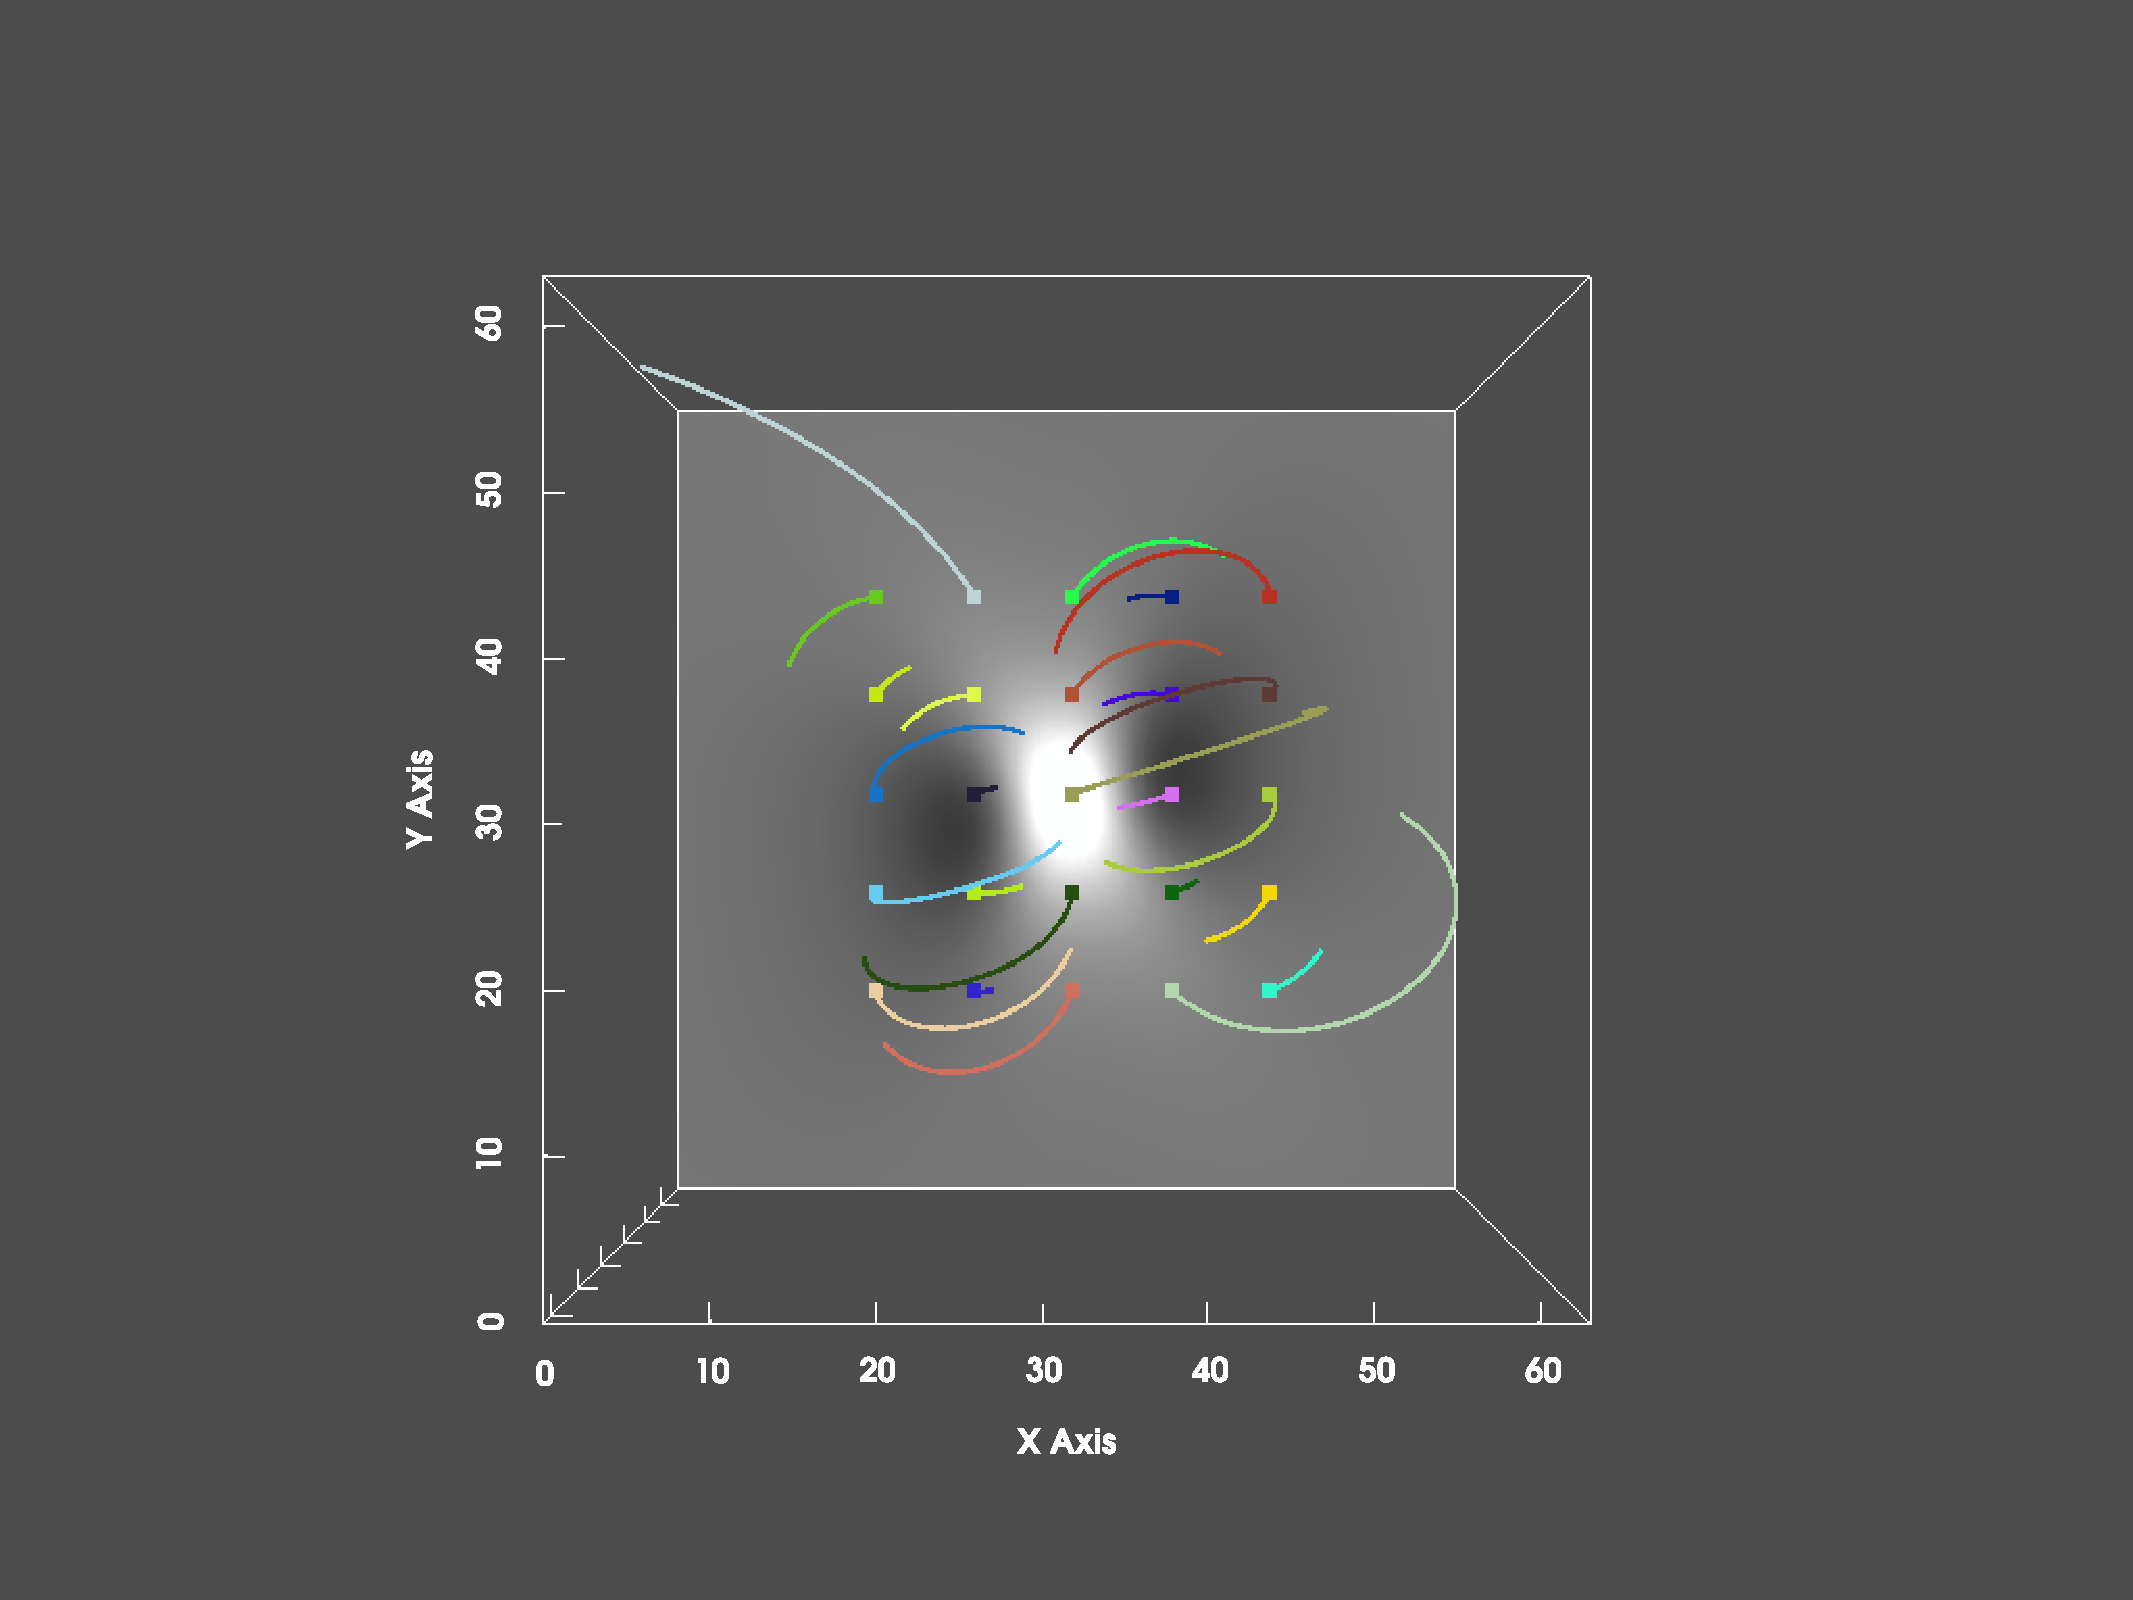
\includegraphics[trim={6cm 1cm 6cm 2cm}, clip, width=\linewidth]{"img/LL_pot_xy.pdf"}
  \end{subfigure}%
  \begin{subfigure}{.5\linewidth}
    \centering
    \caption{Low-Lou}
    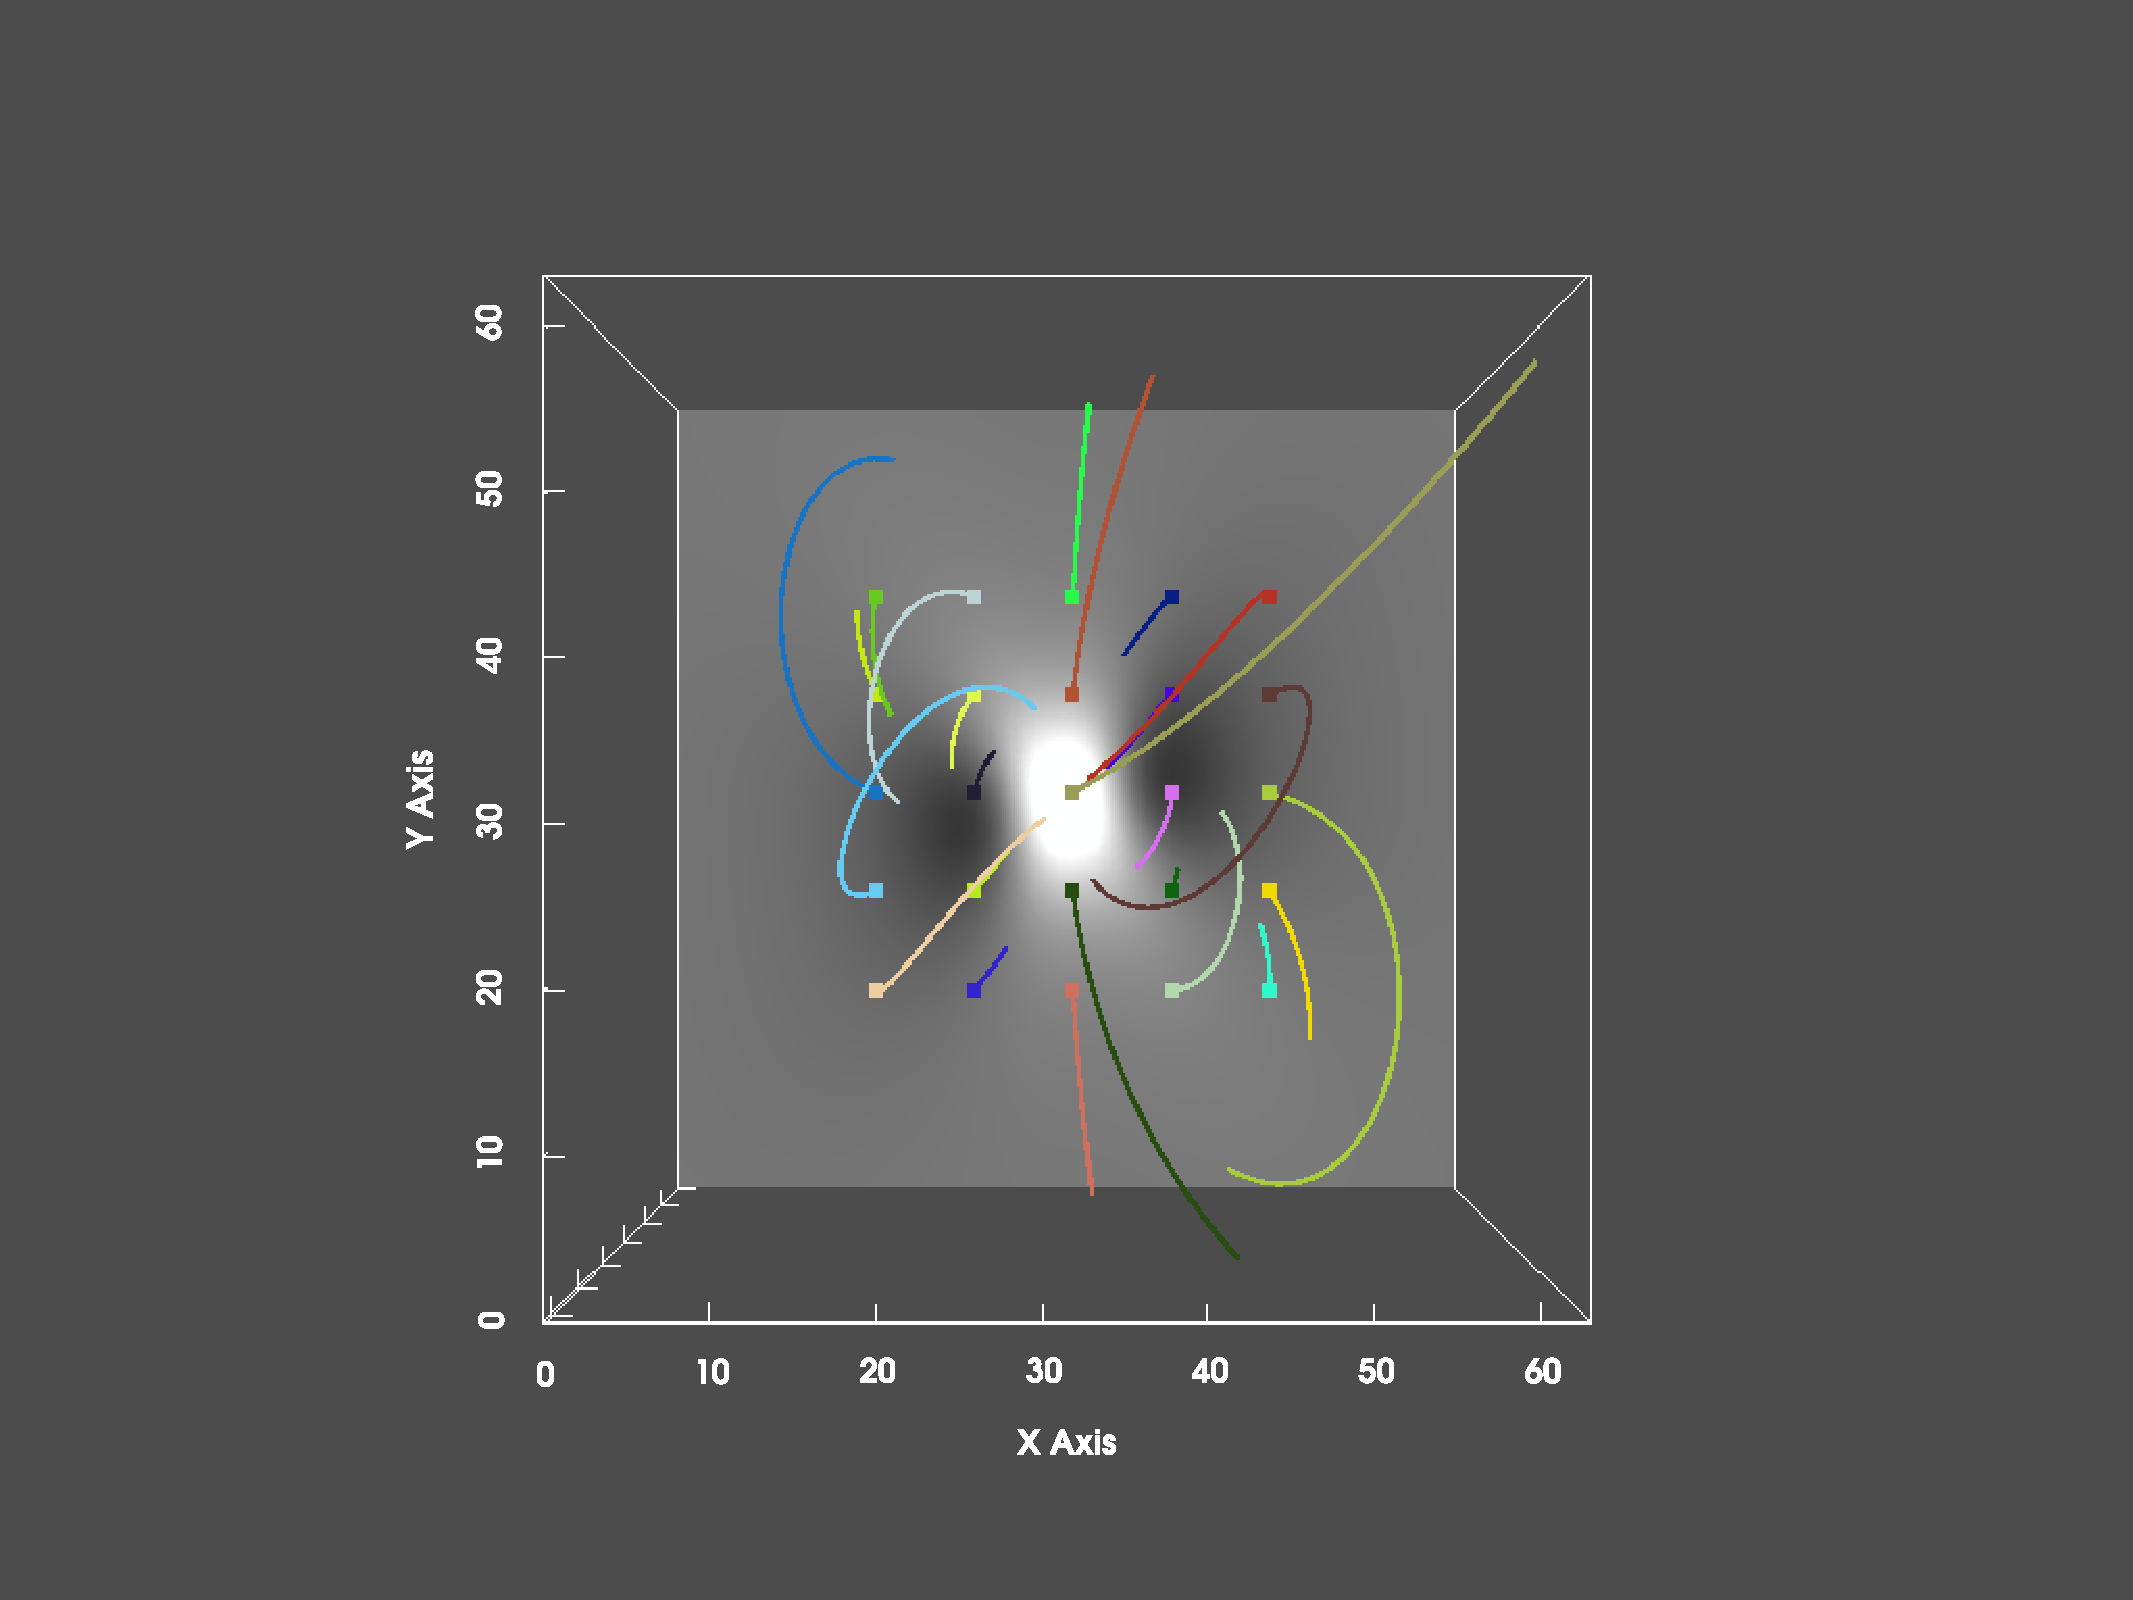
\includegraphics[trim={6cm 1cm 6cm 2cm}, clip, width=\linewidth]{"img/LL_xy.pdf"}
  \end{subfigure}
  
  \caption{The magnetic fields in the xy plane. Each field line is distinguished by its unique color, which is determined by its footpoint at $z=0$ plane.}\label{fig:xy}
\end{figure}

\begin{figure}
  \begin{subfigure}{.5\linewidth}
    \centering
    \caption{PINN(0)}\label{fig:yz0}
    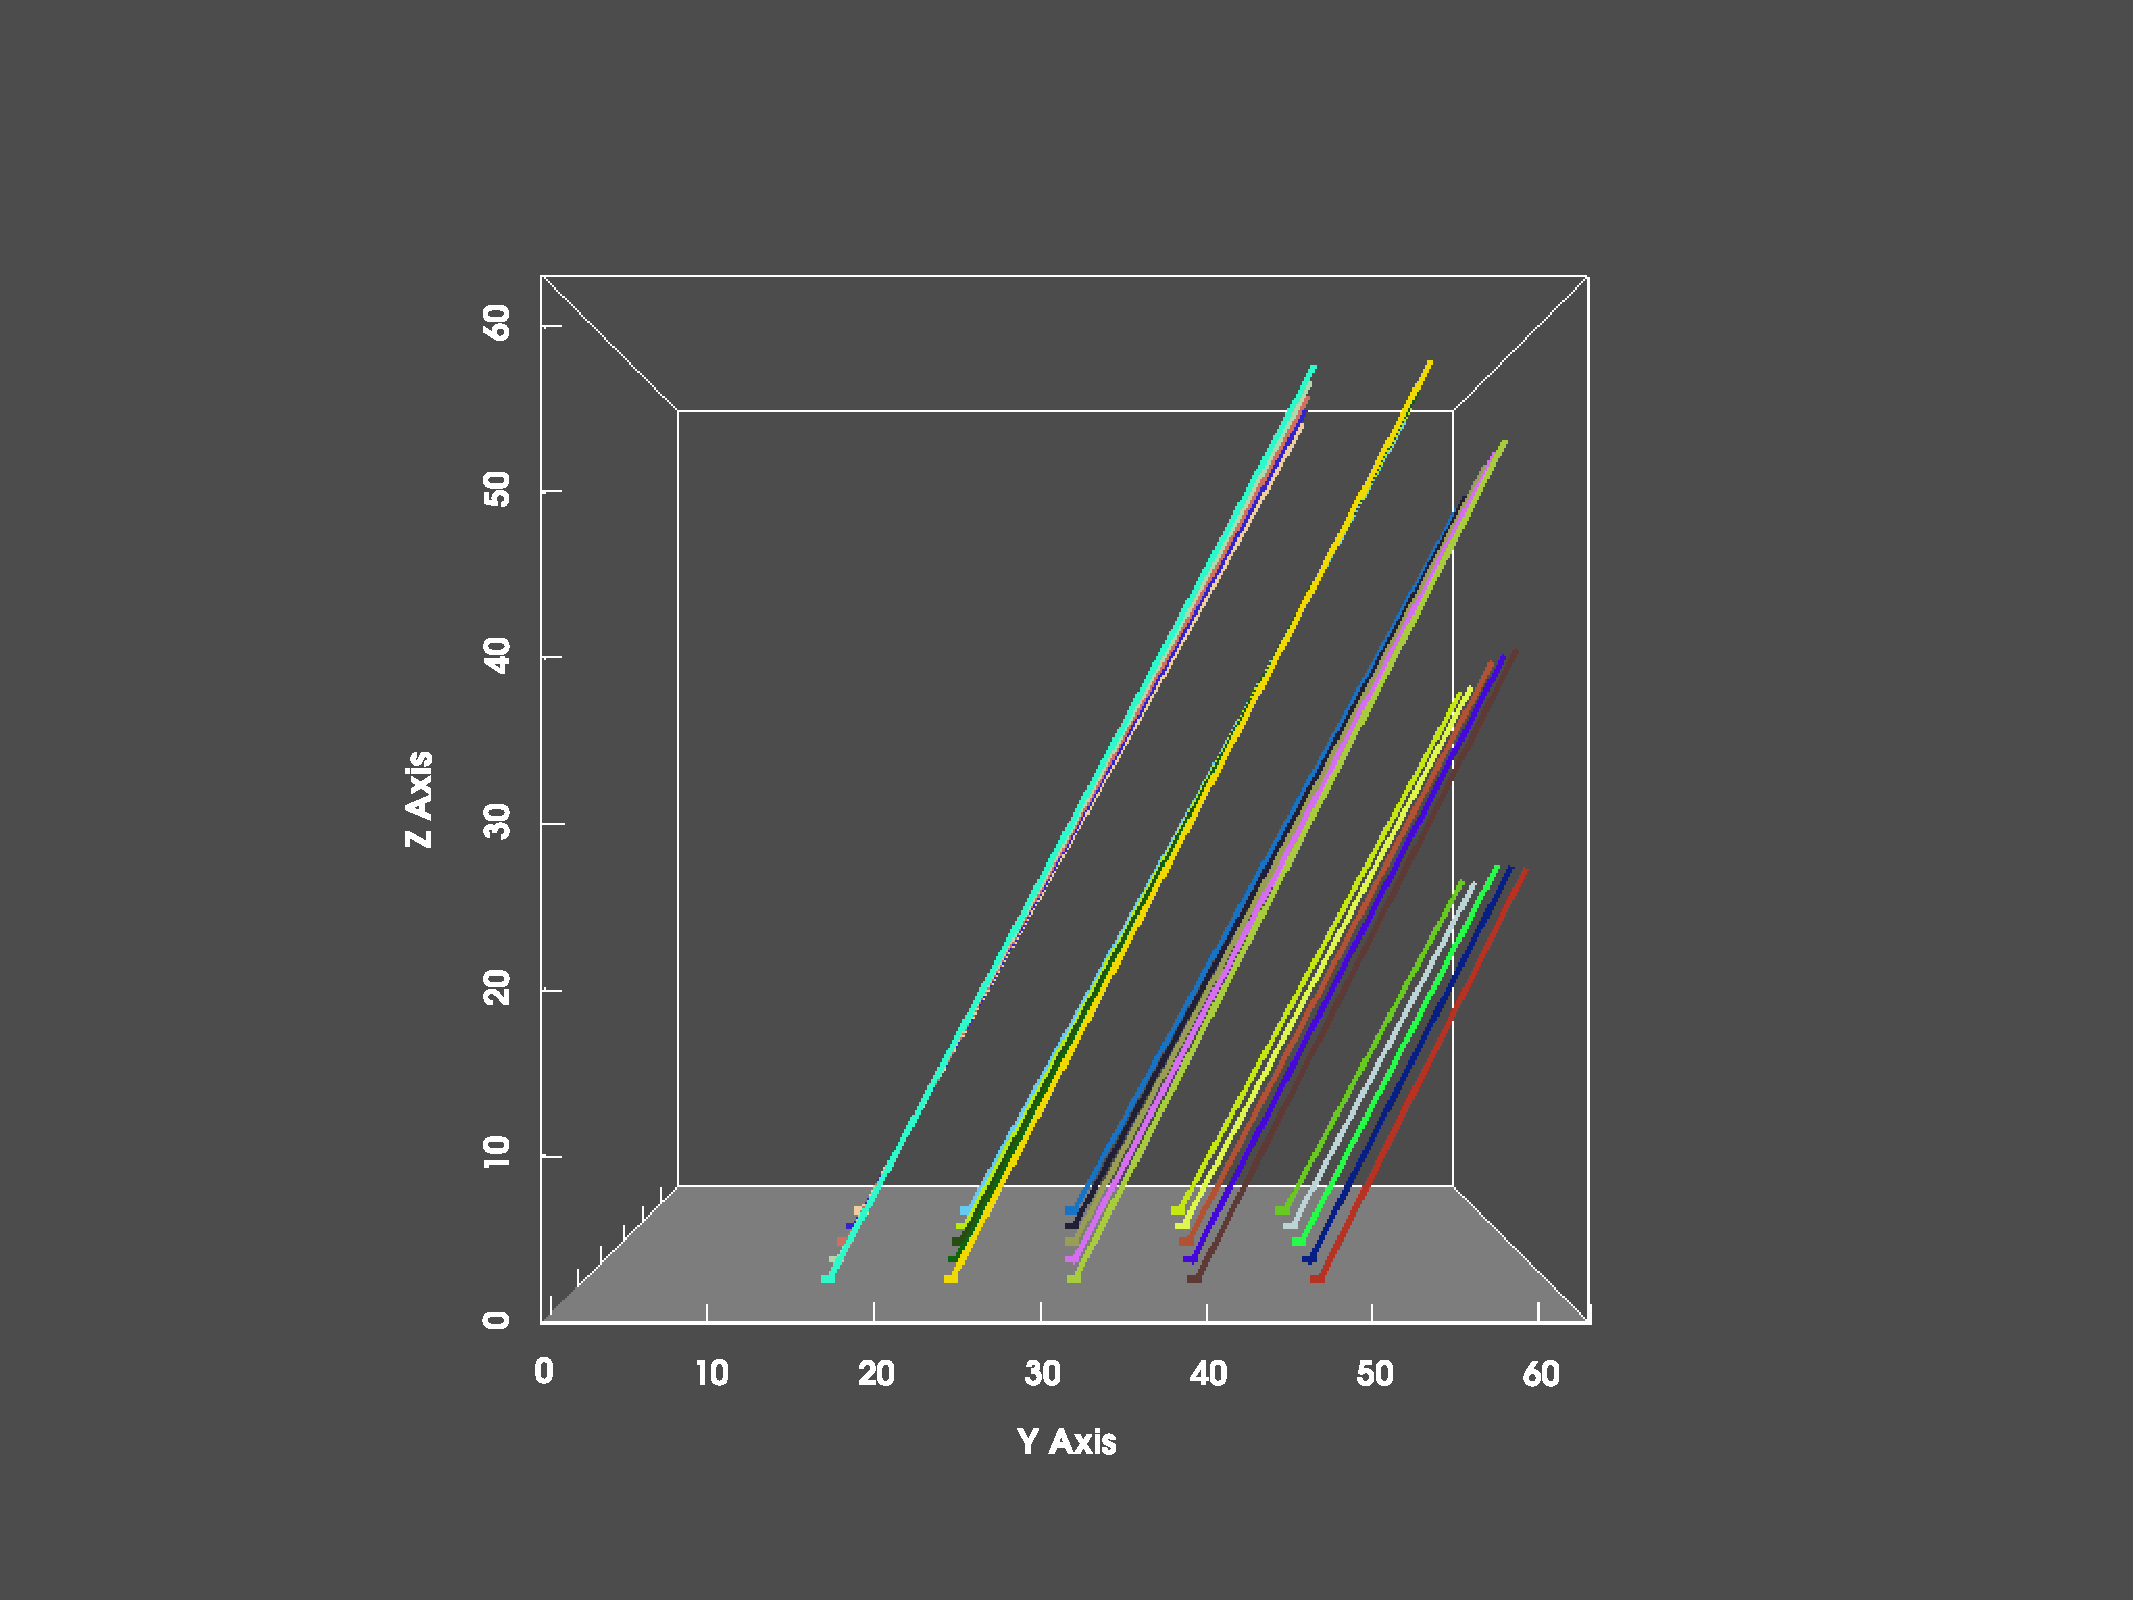
\includegraphics[trim={6cm 1cm 6cm 2cm}, clip, width=\linewidth]{"img/PINN_000000_yz.pdf"}
  \end{subfigure}%
  \begin{subfigure}{.5\linewidth}
    \centering
    \caption{PINN(100)}
    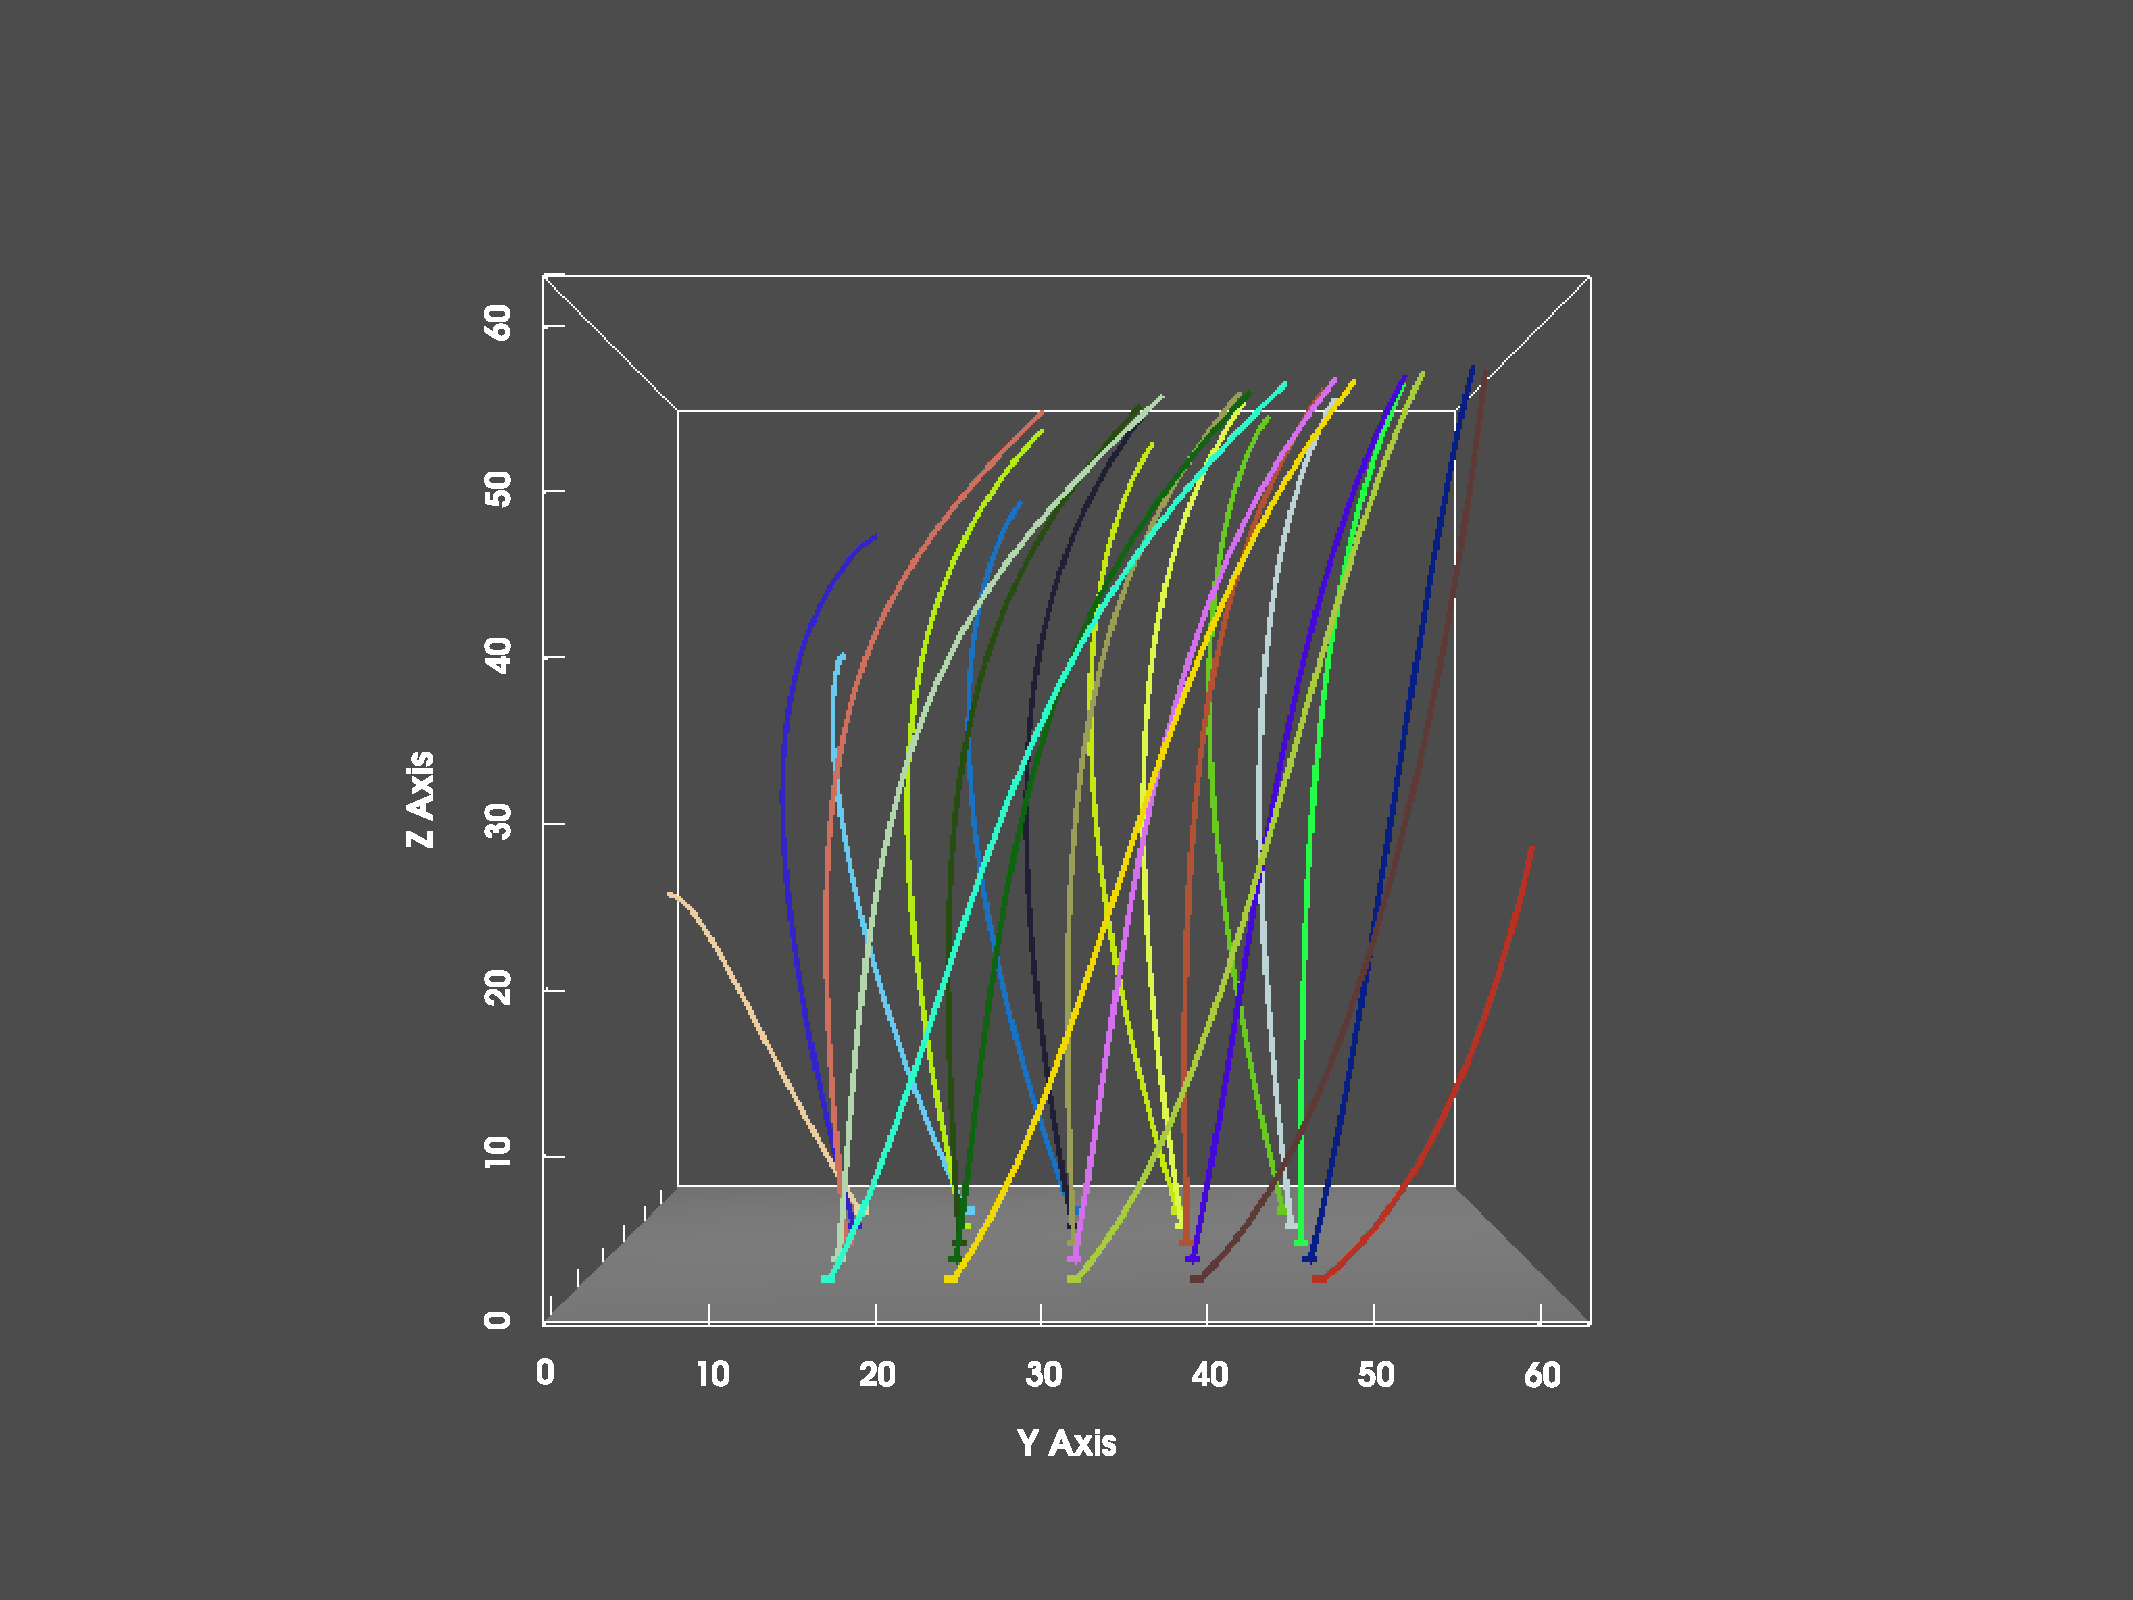
\includegraphics[trim={6cm 1cm 6cm 2cm}, clip, width=\linewidth]{"img/PINN_000100_yz.pdf"}
  \end{subfigure}

  \begin{subfigure}{.5\linewidth}
    \centering
    \caption{PINN(1000)}
    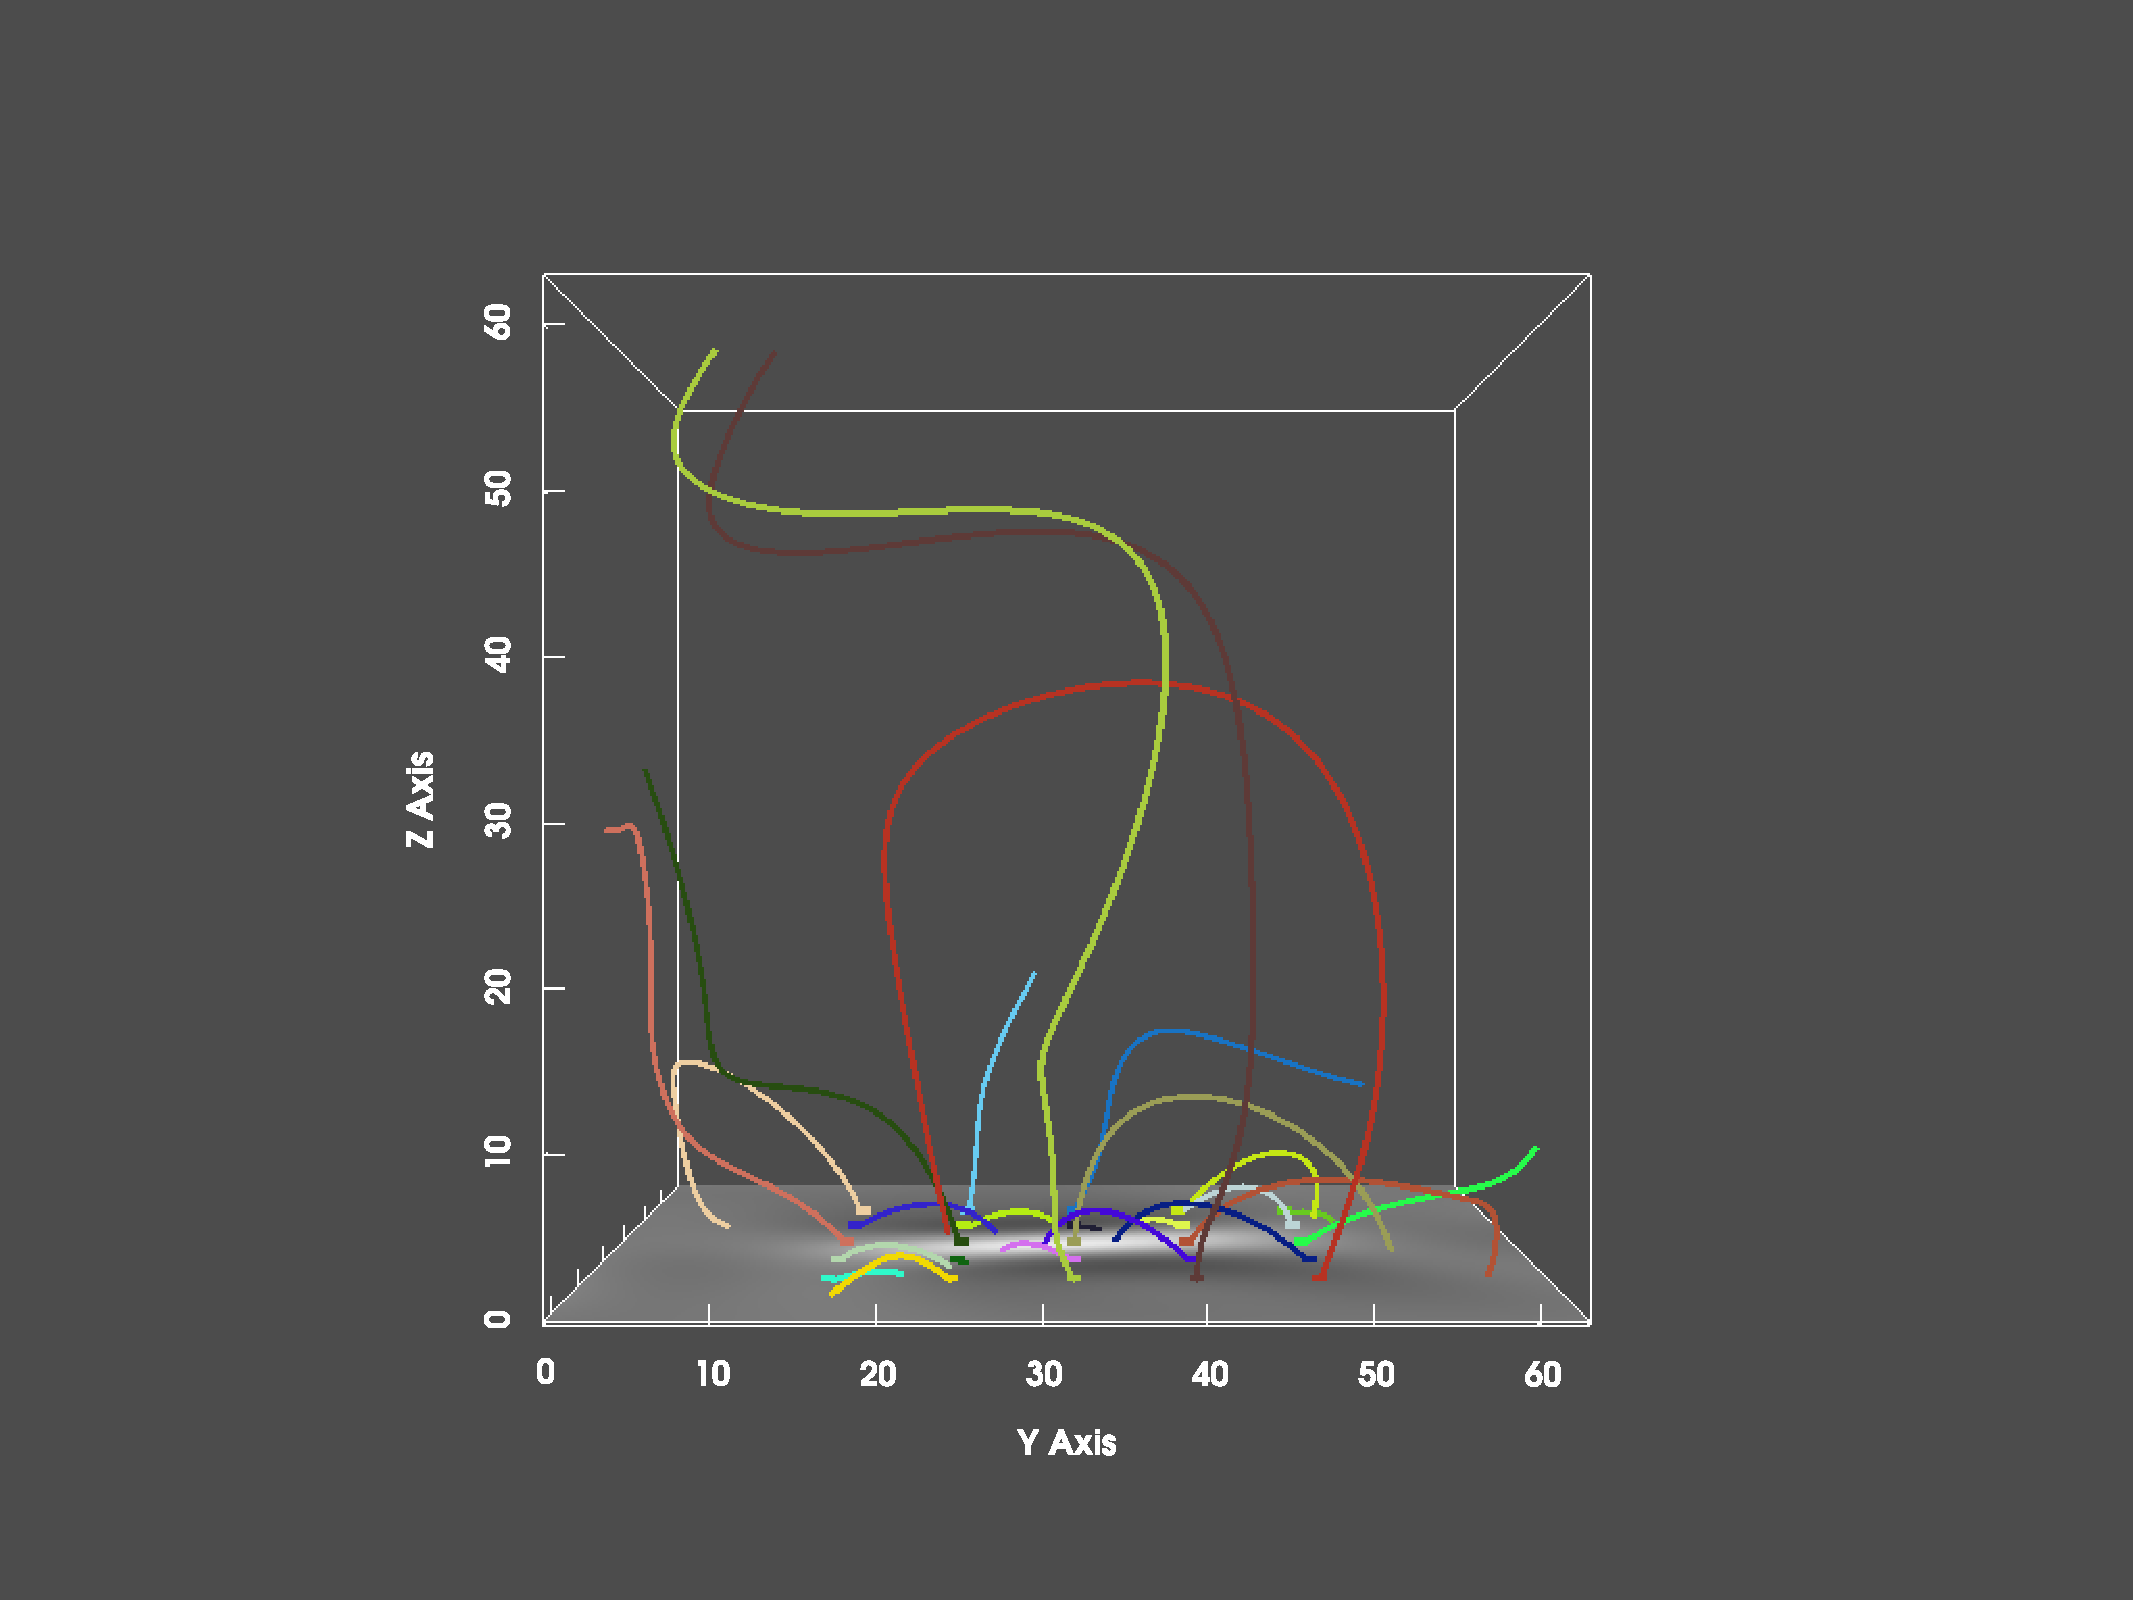
\includegraphics[trim={6cm 1cm 6cm 2cm}, clip, width=\linewidth]{"img/PINN_001000_yz.pdf"}
  \end{subfigure}%
  \begin{subfigure}{.5\linewidth}
    \centering
    \caption{PINN(10000)}
    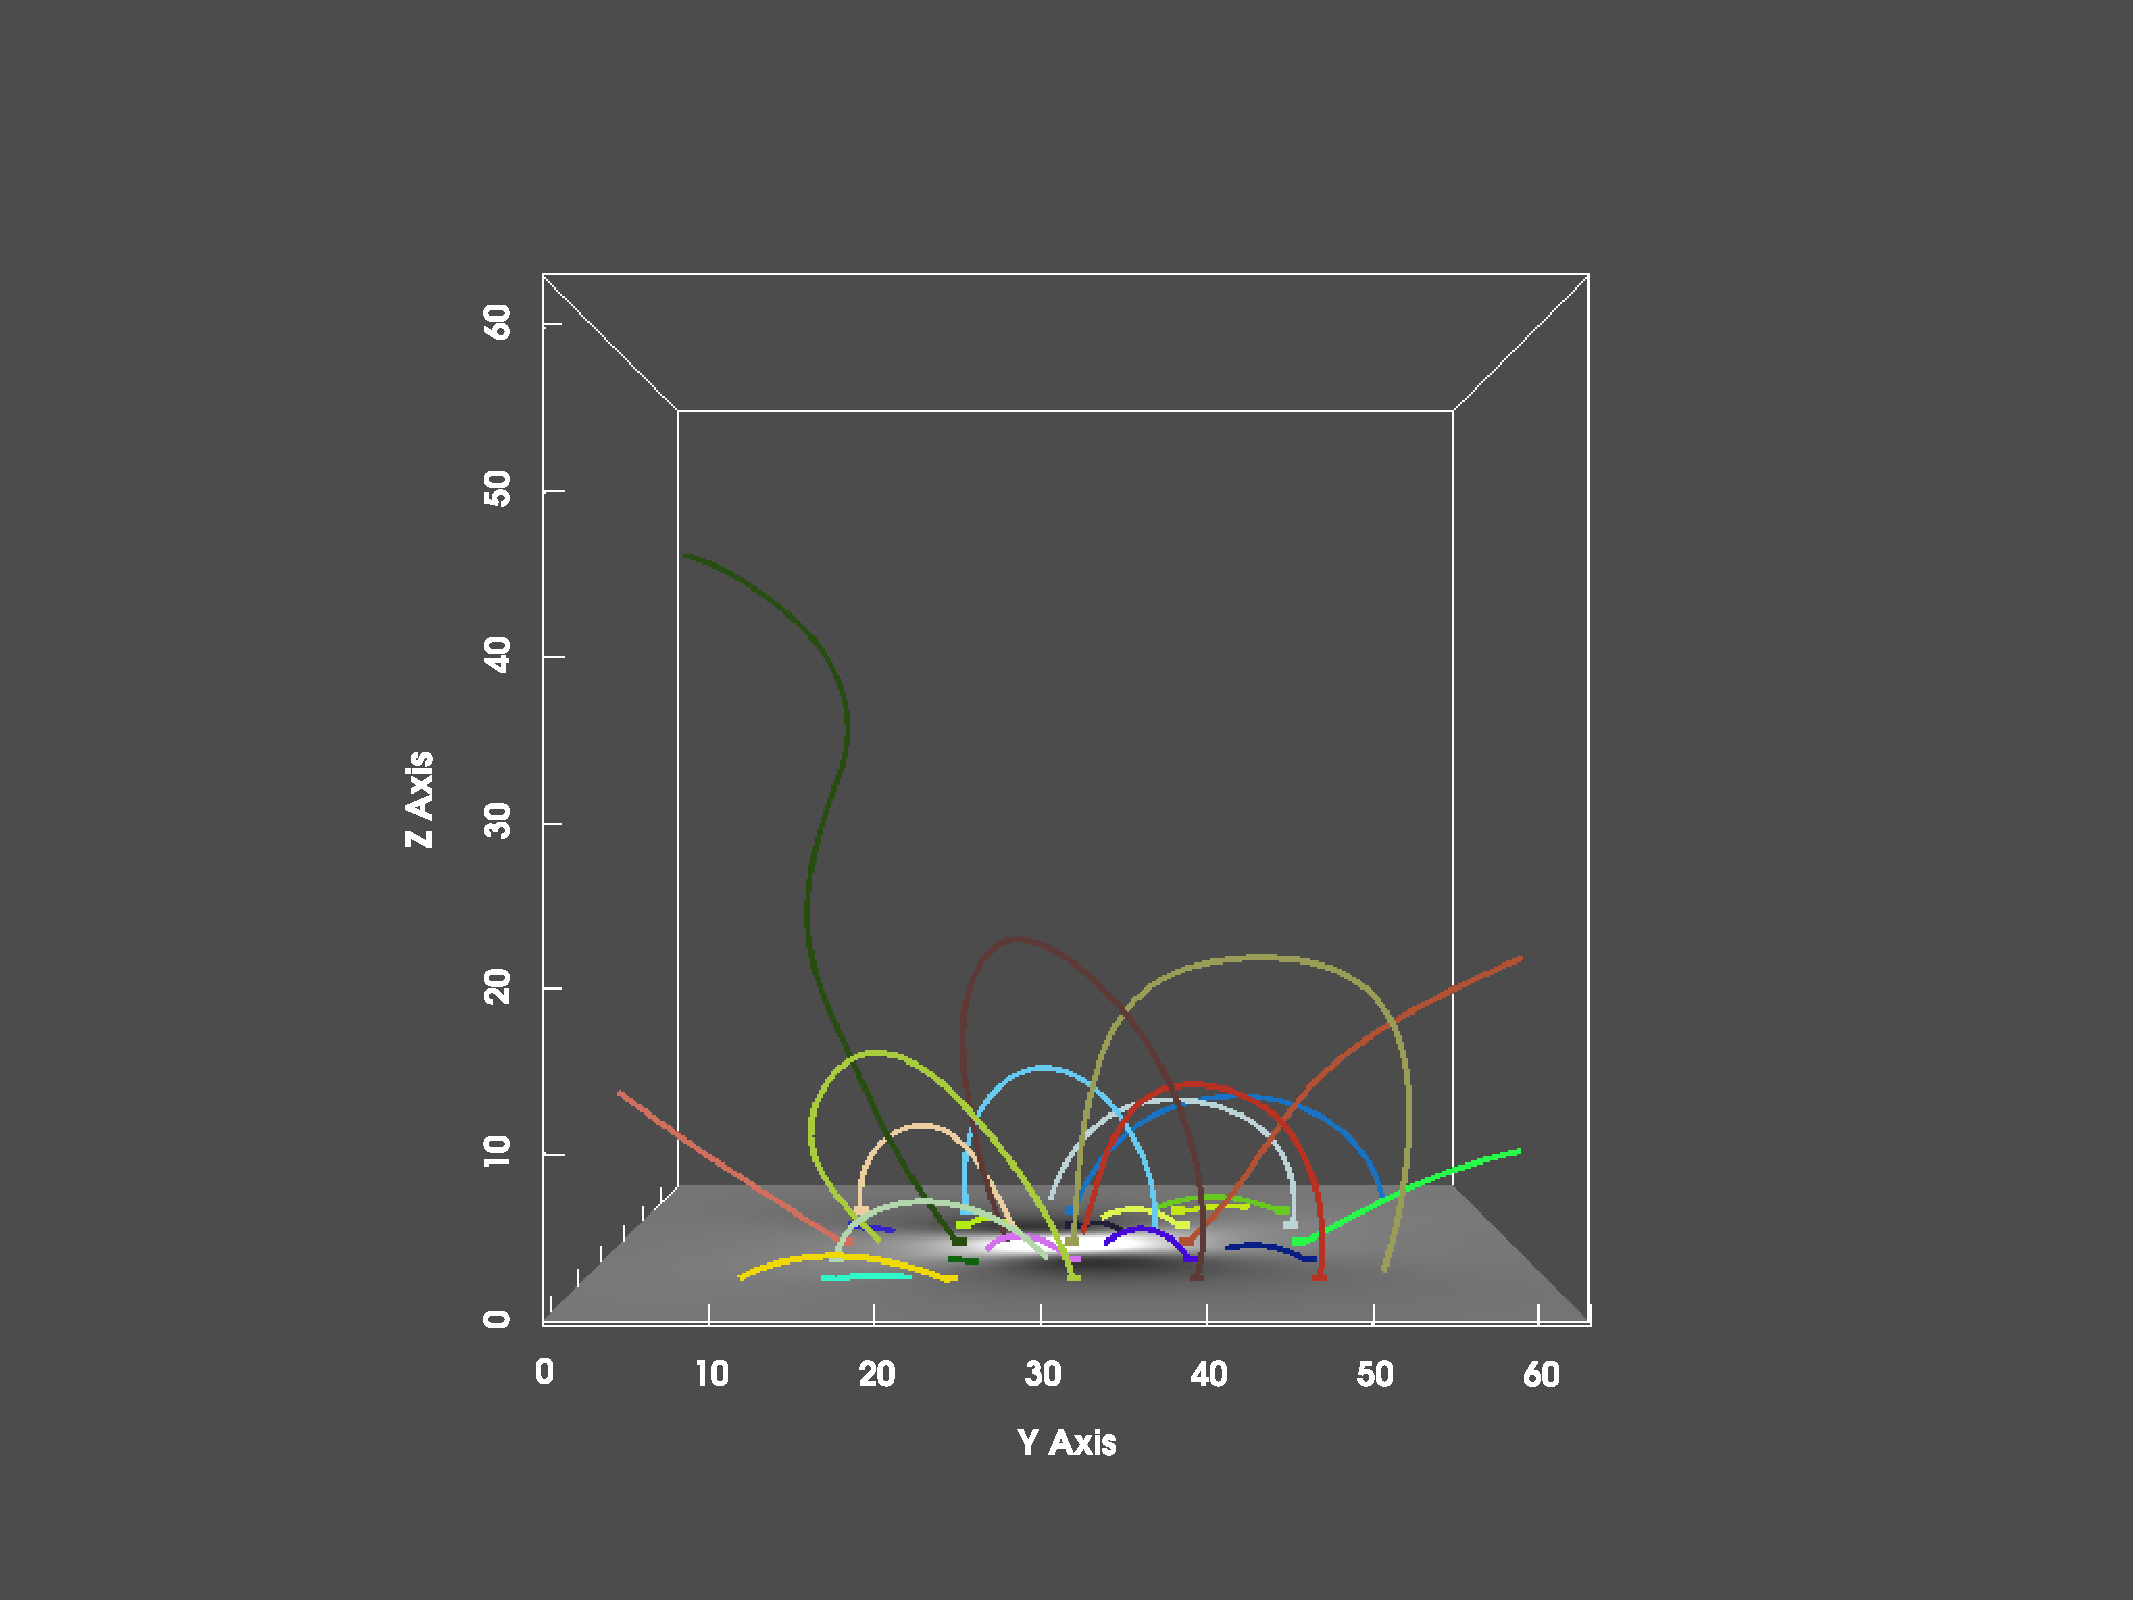
\includegraphics[trim={6cm 1cm 6cm 2cm}, clip, width=\linewidth]{"img/PINN_010000_yz.pdf"}
  \end{subfigure}

  \begin{subfigure}{.5\linewidth}
    \centering
    \caption{PINN(25000)}
    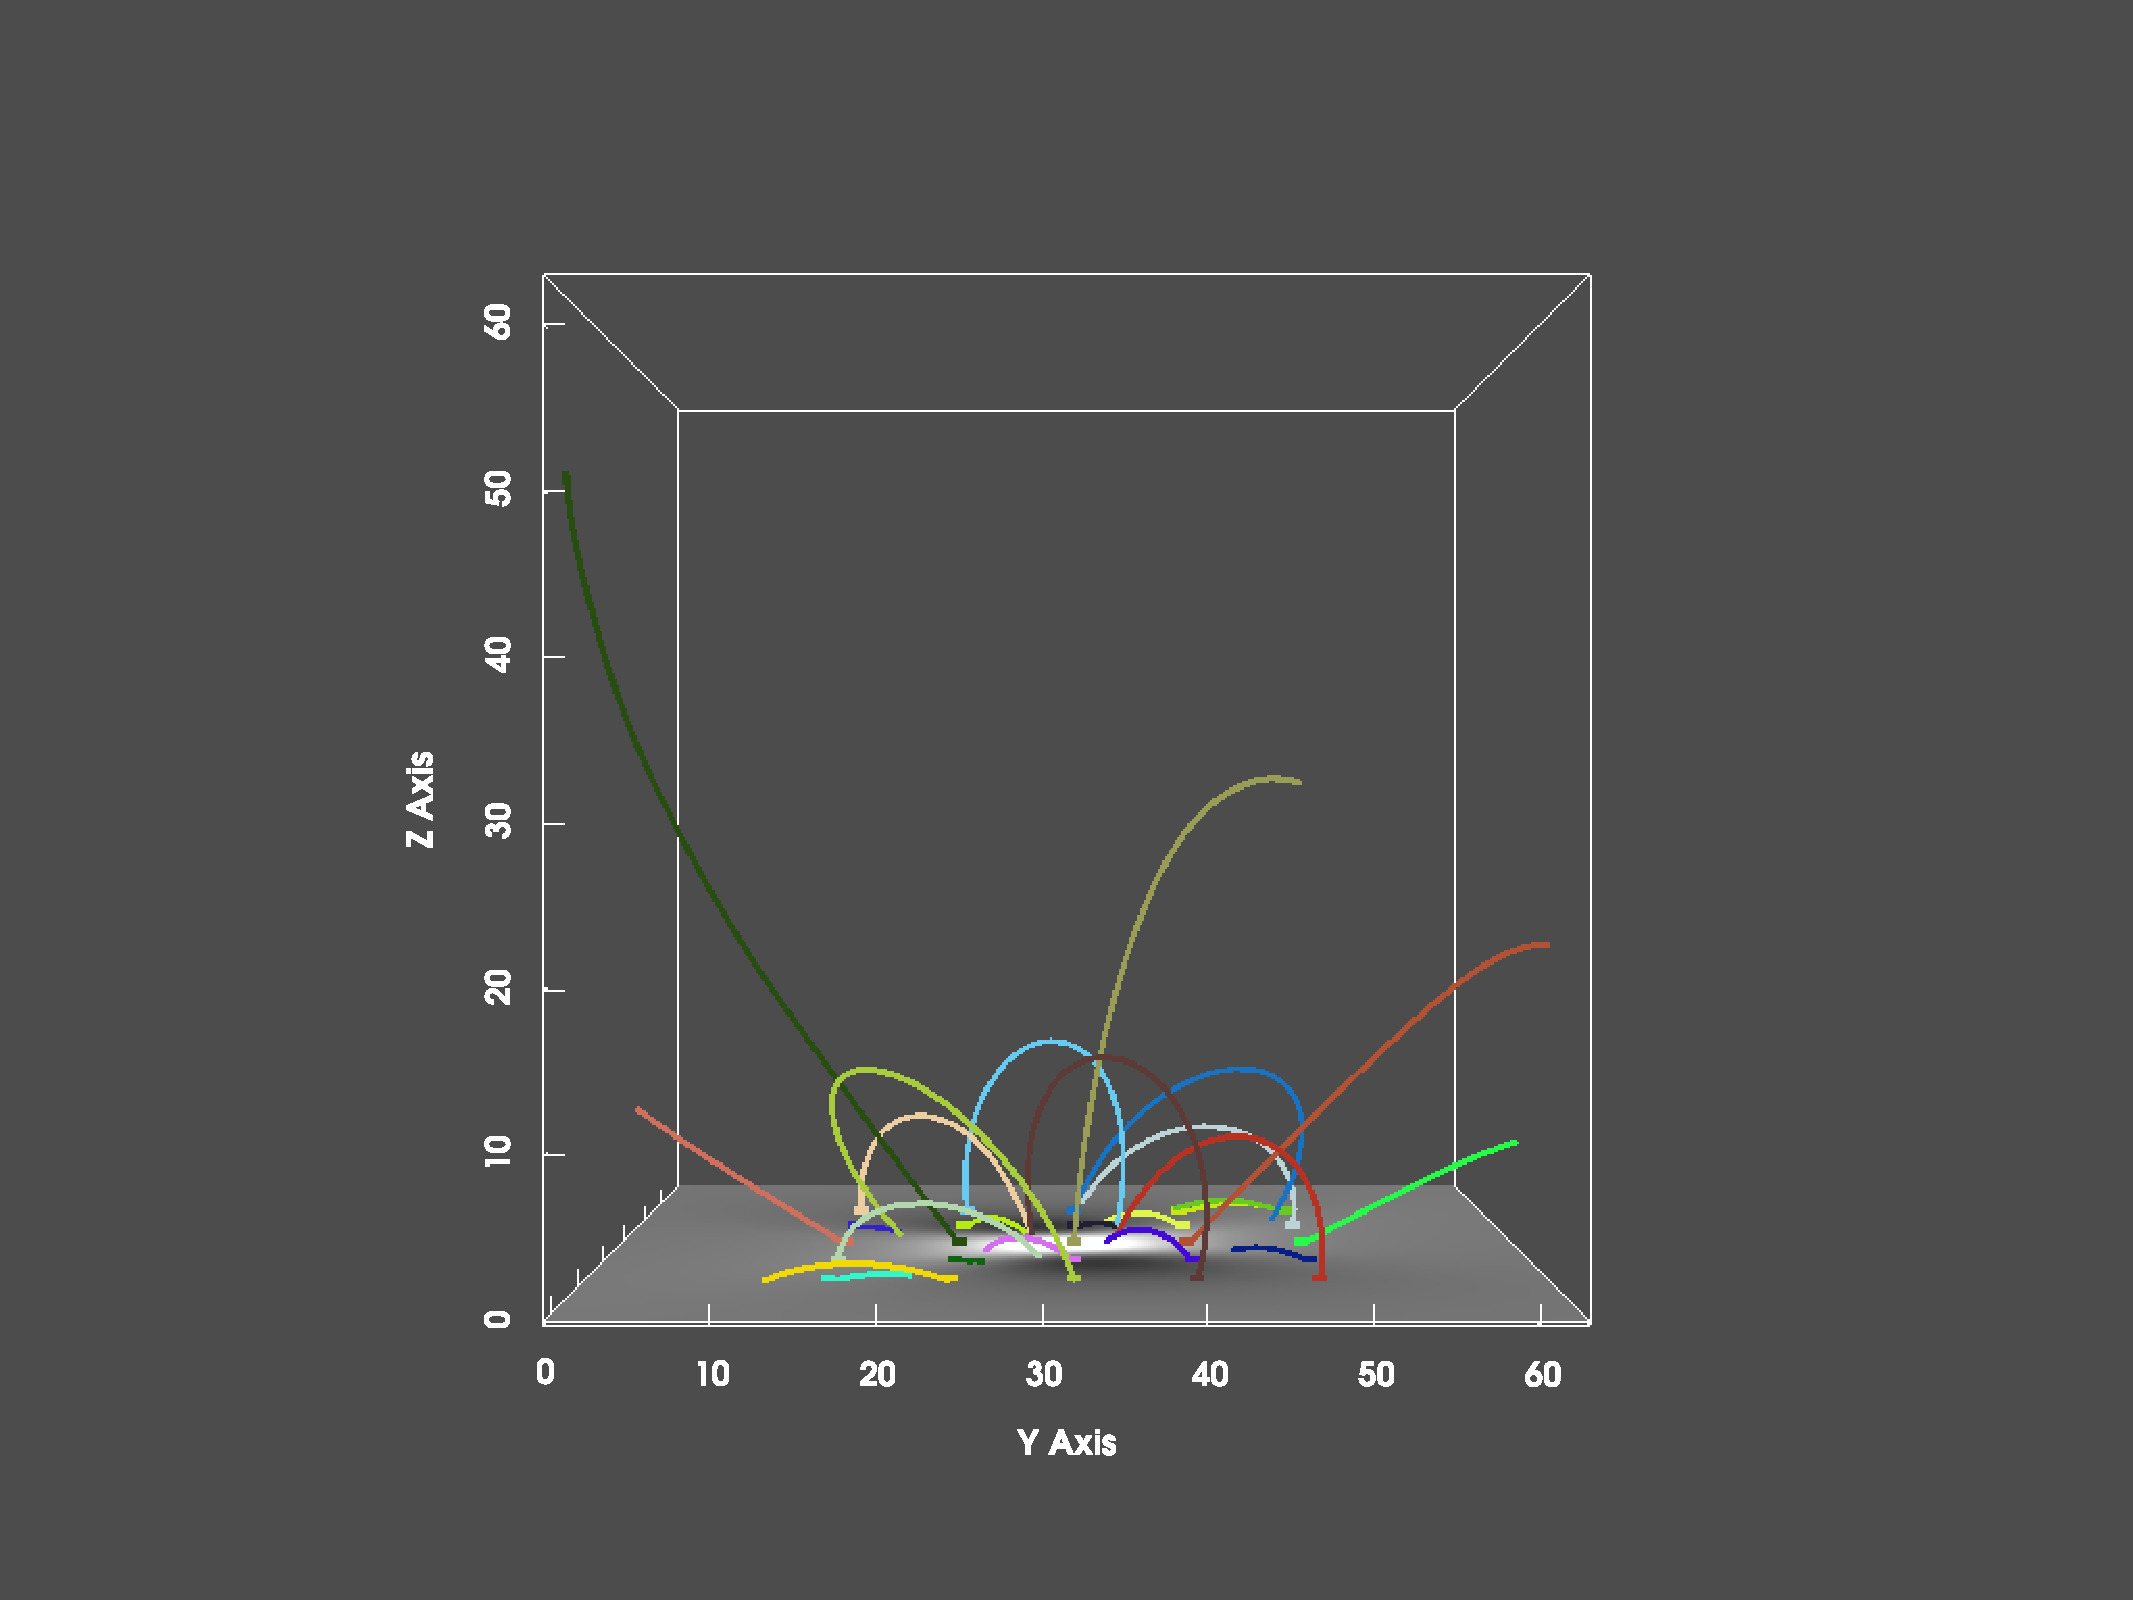
\includegraphics[trim={6cm 1cm 6cm 2cm}, clip, width=\linewidth]{"img/PINN_025000_yz.pdf"}
  \end{subfigure}%
  \begin{subfigure}{.5\linewidth}
    \centering
    \caption{PINN(50000)}
    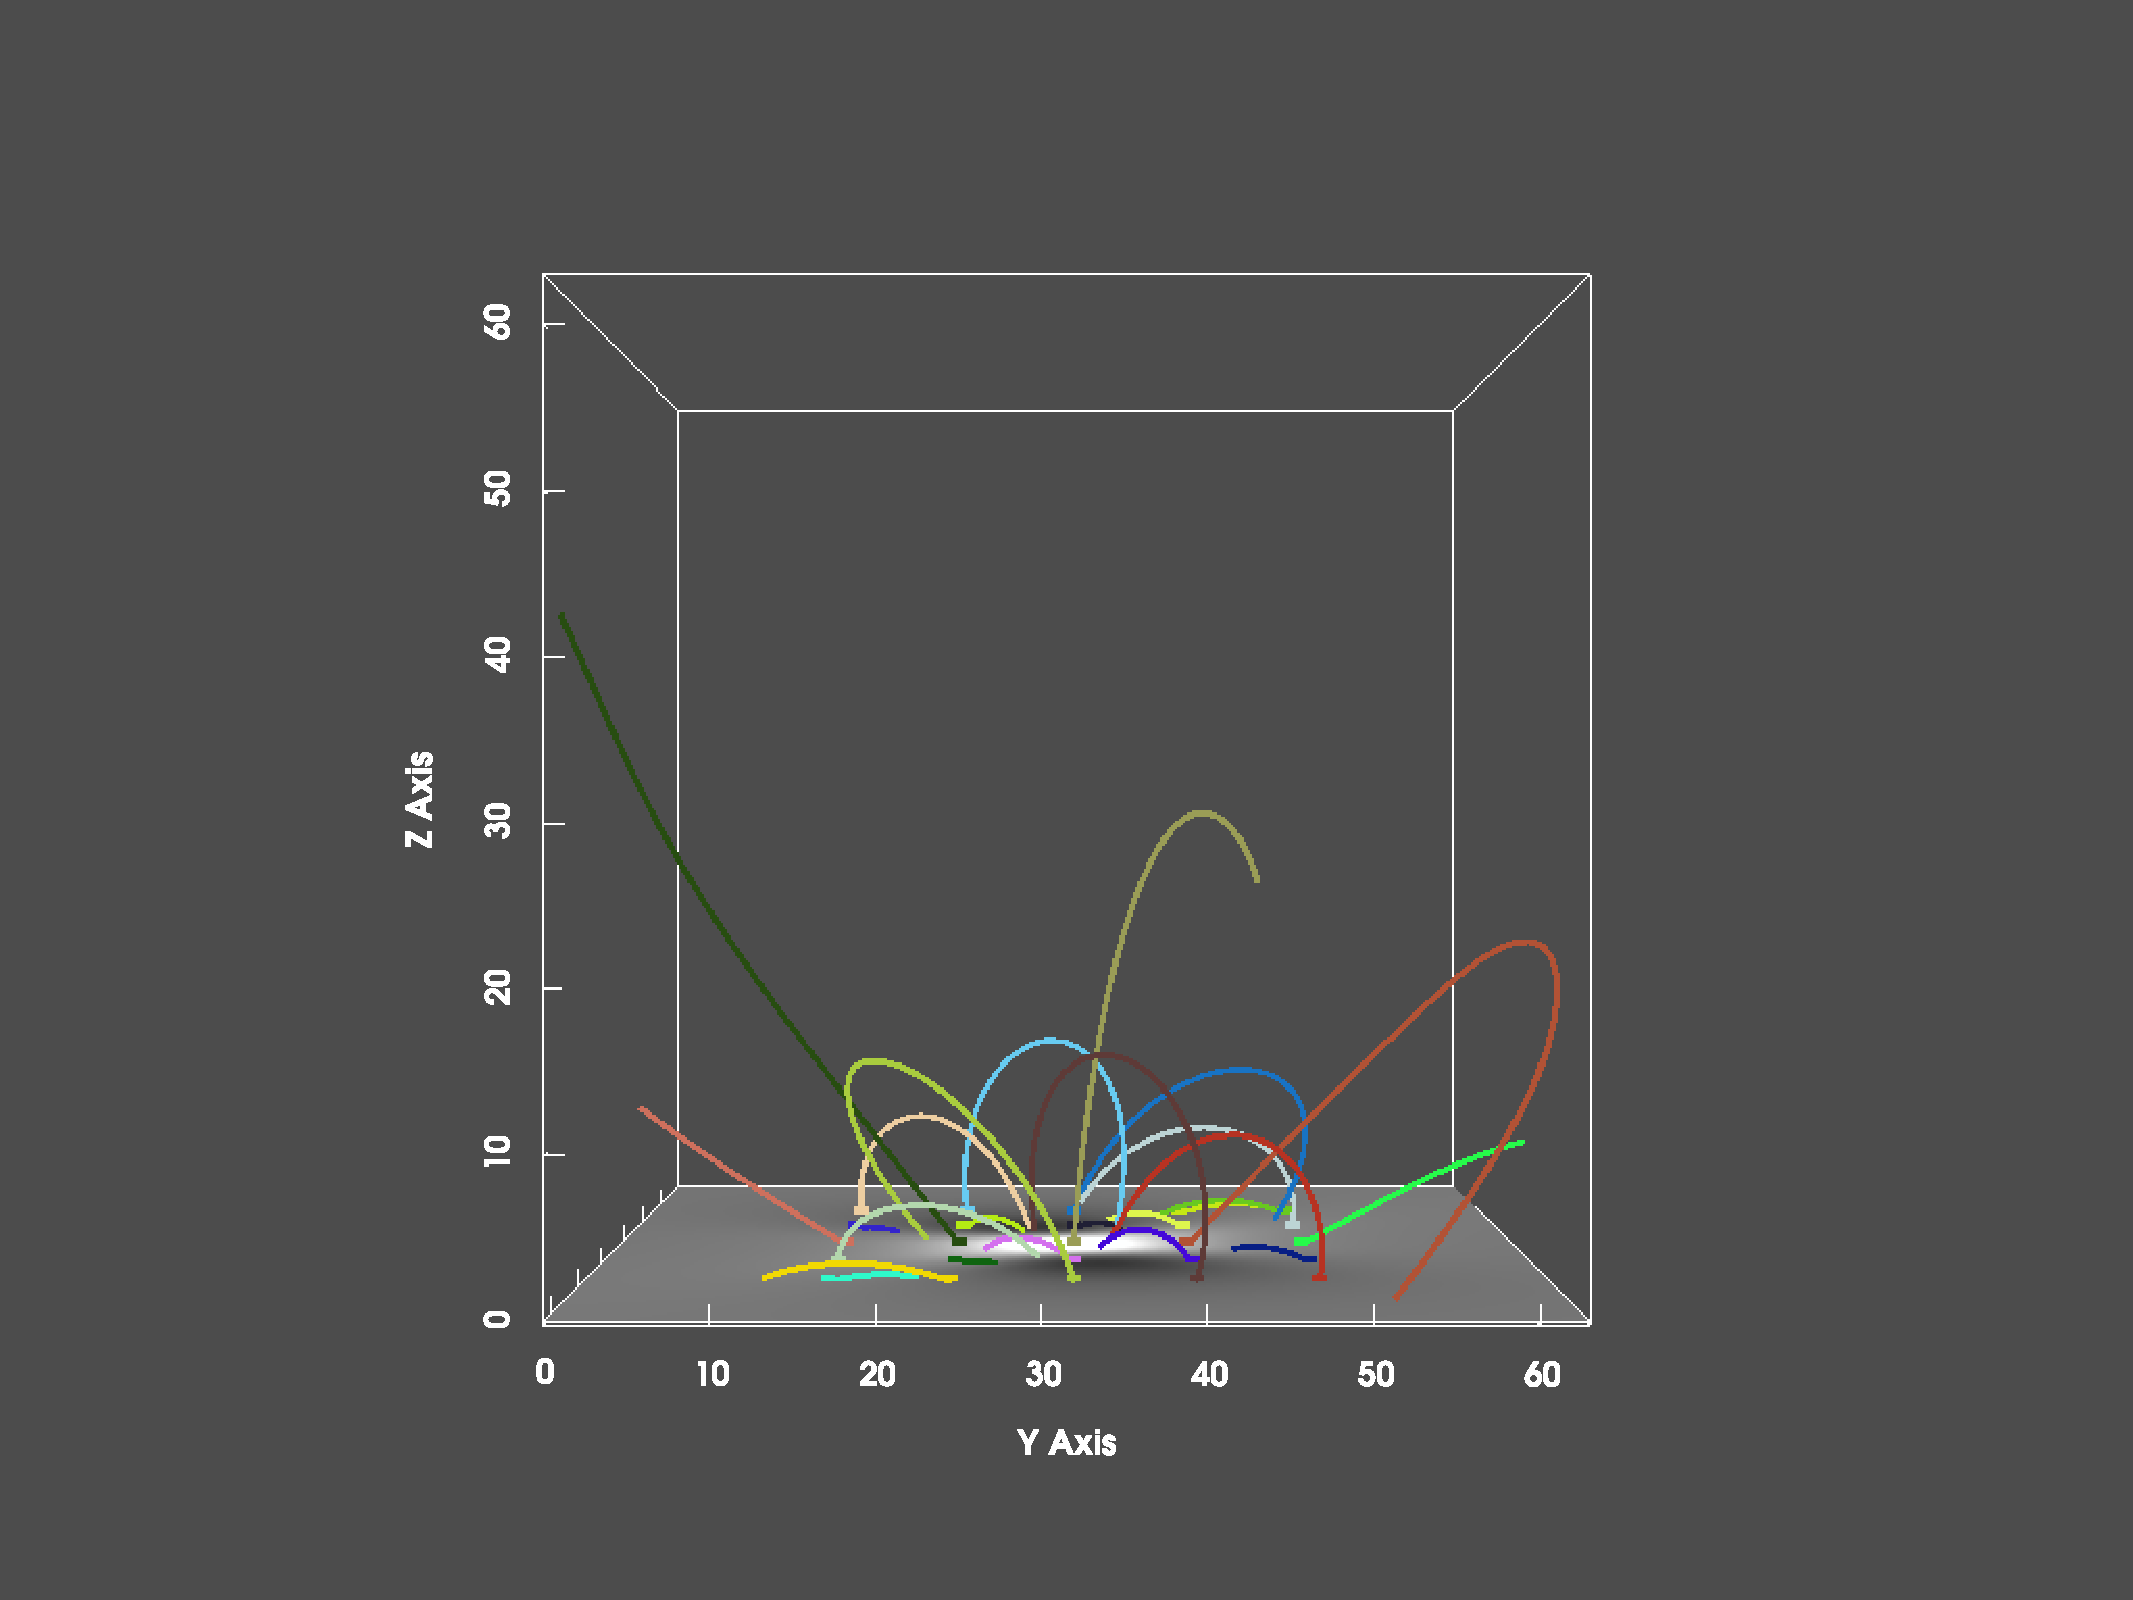
\includegraphics[trim={6cm 1cm 6cm 2cm}, clip, width=\linewidth]{"img/PINN_050000_yz.pdf"}
  \end{subfigure}
  
  \begin{subfigure}{.5\linewidth}
    \centering
    \caption{Potential}
    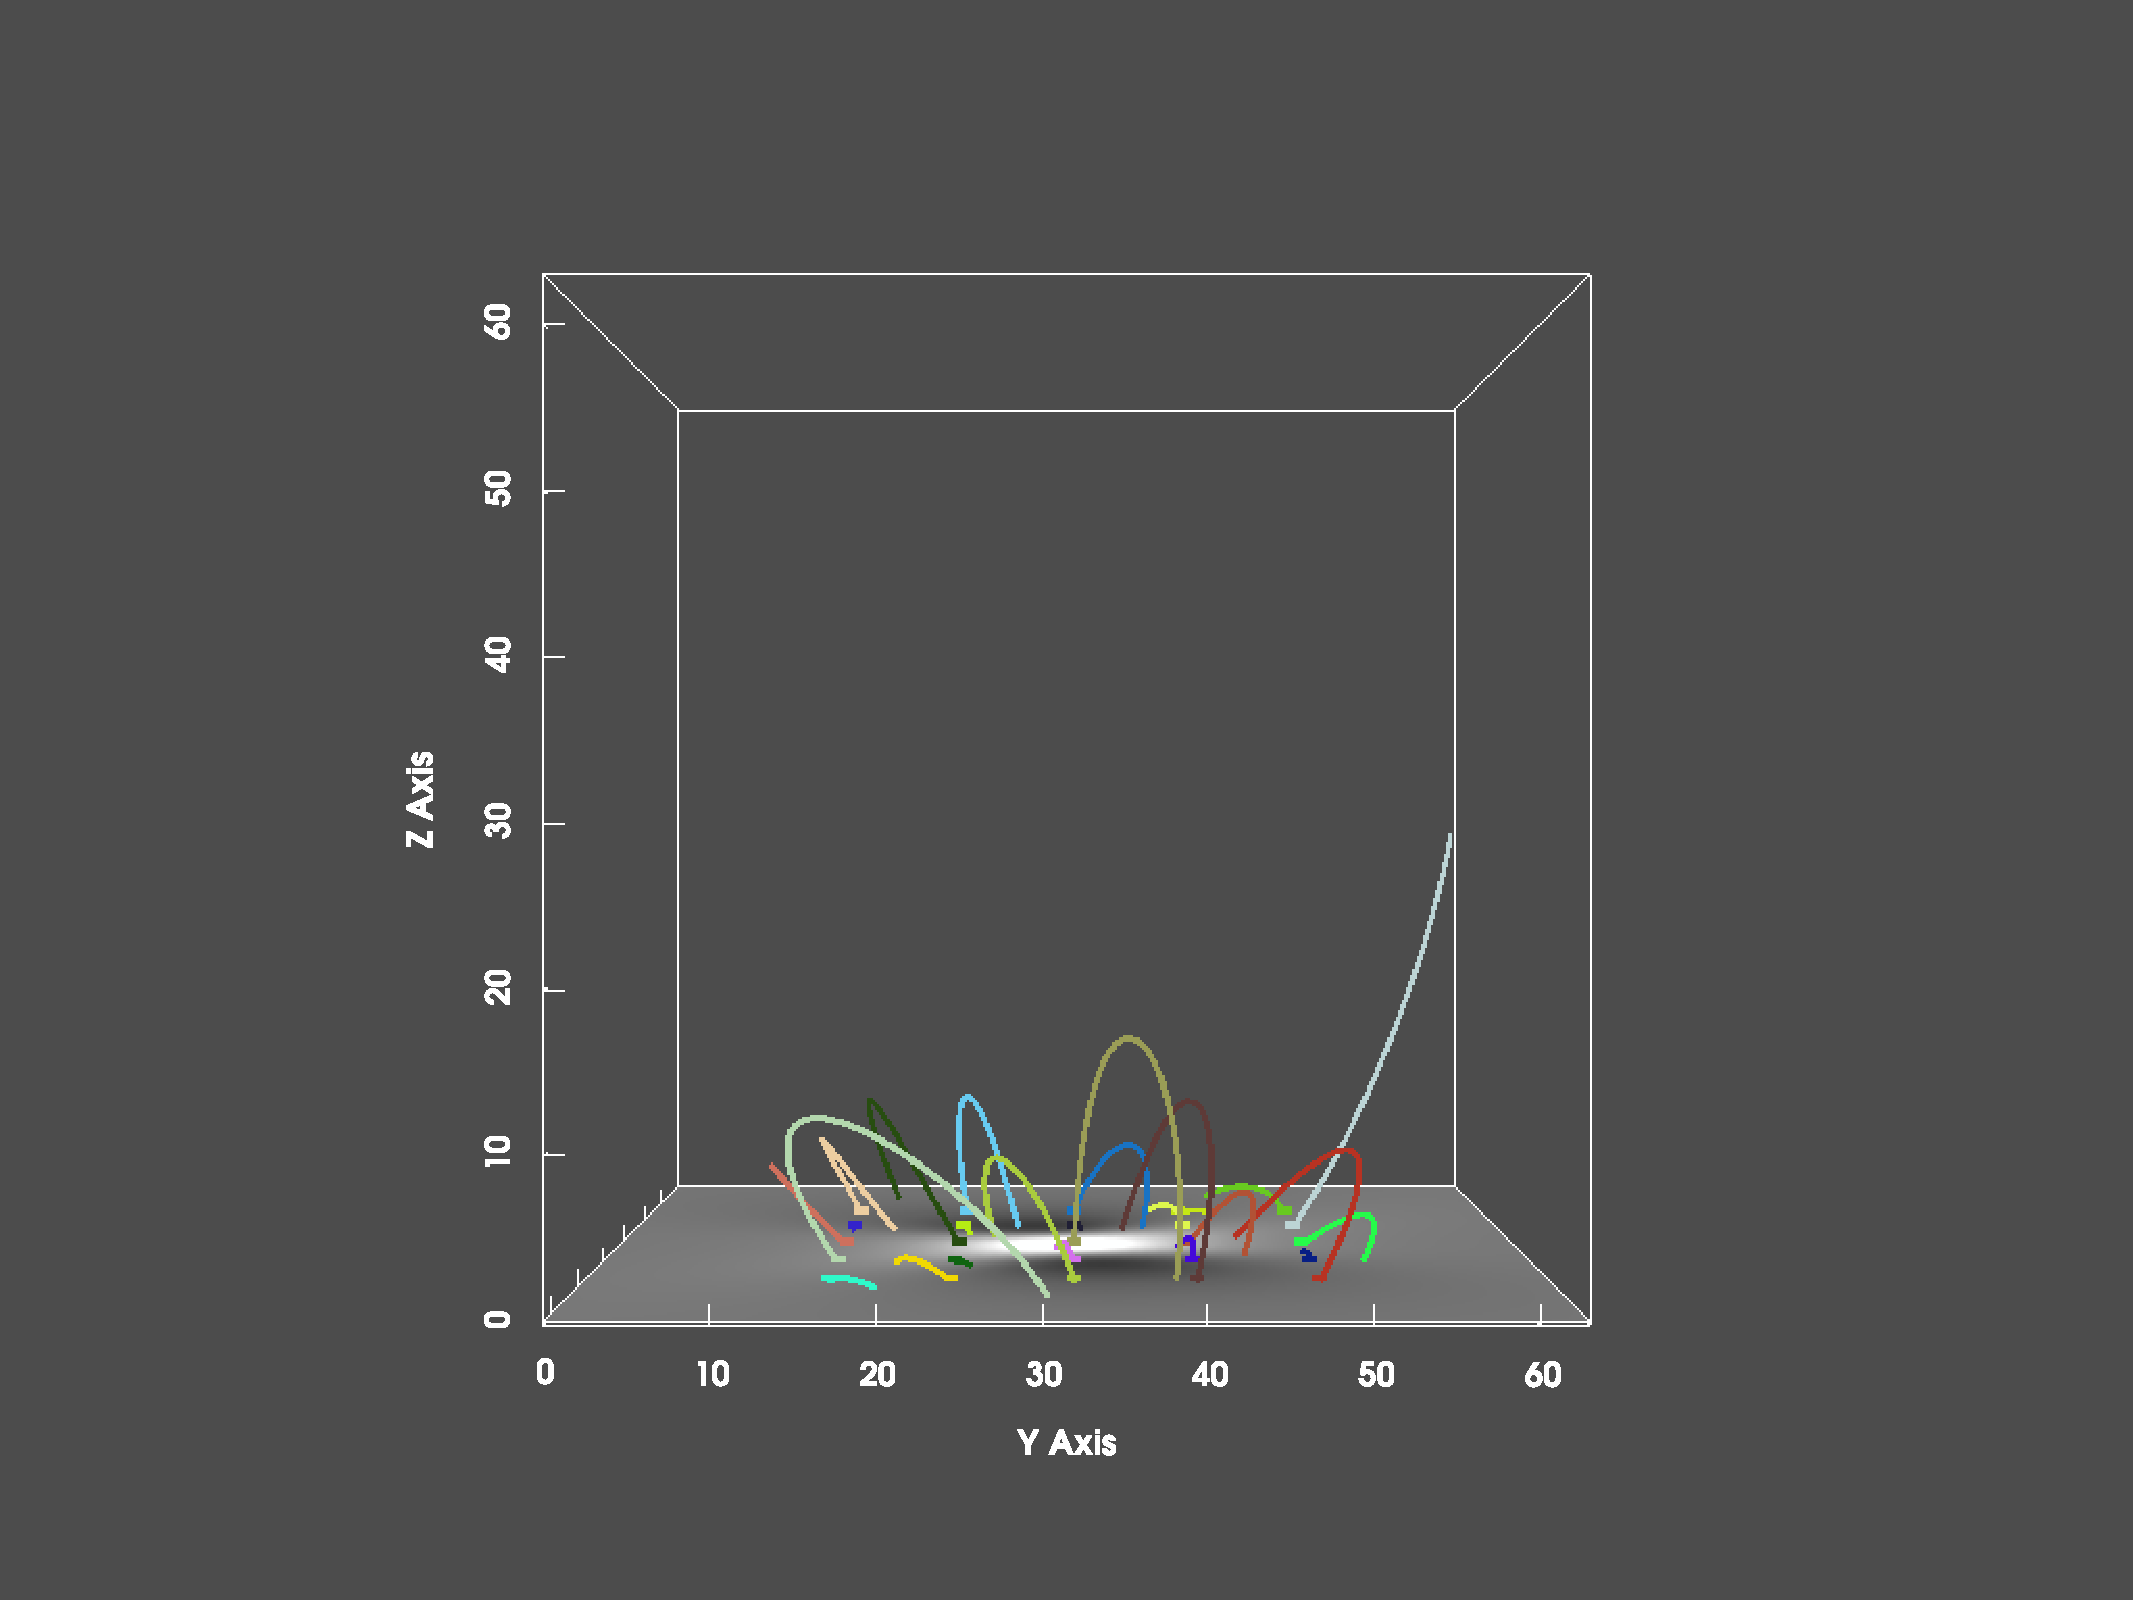
\includegraphics[trim={6cm 1cm 6cm 2cm}, clip, width=\linewidth]{"img/LL_pot_yz.pdf"}
  \end{subfigure}%
  \begin{subfigure}{.5\linewidth}
    \centering
    \caption{Low-Lou}
    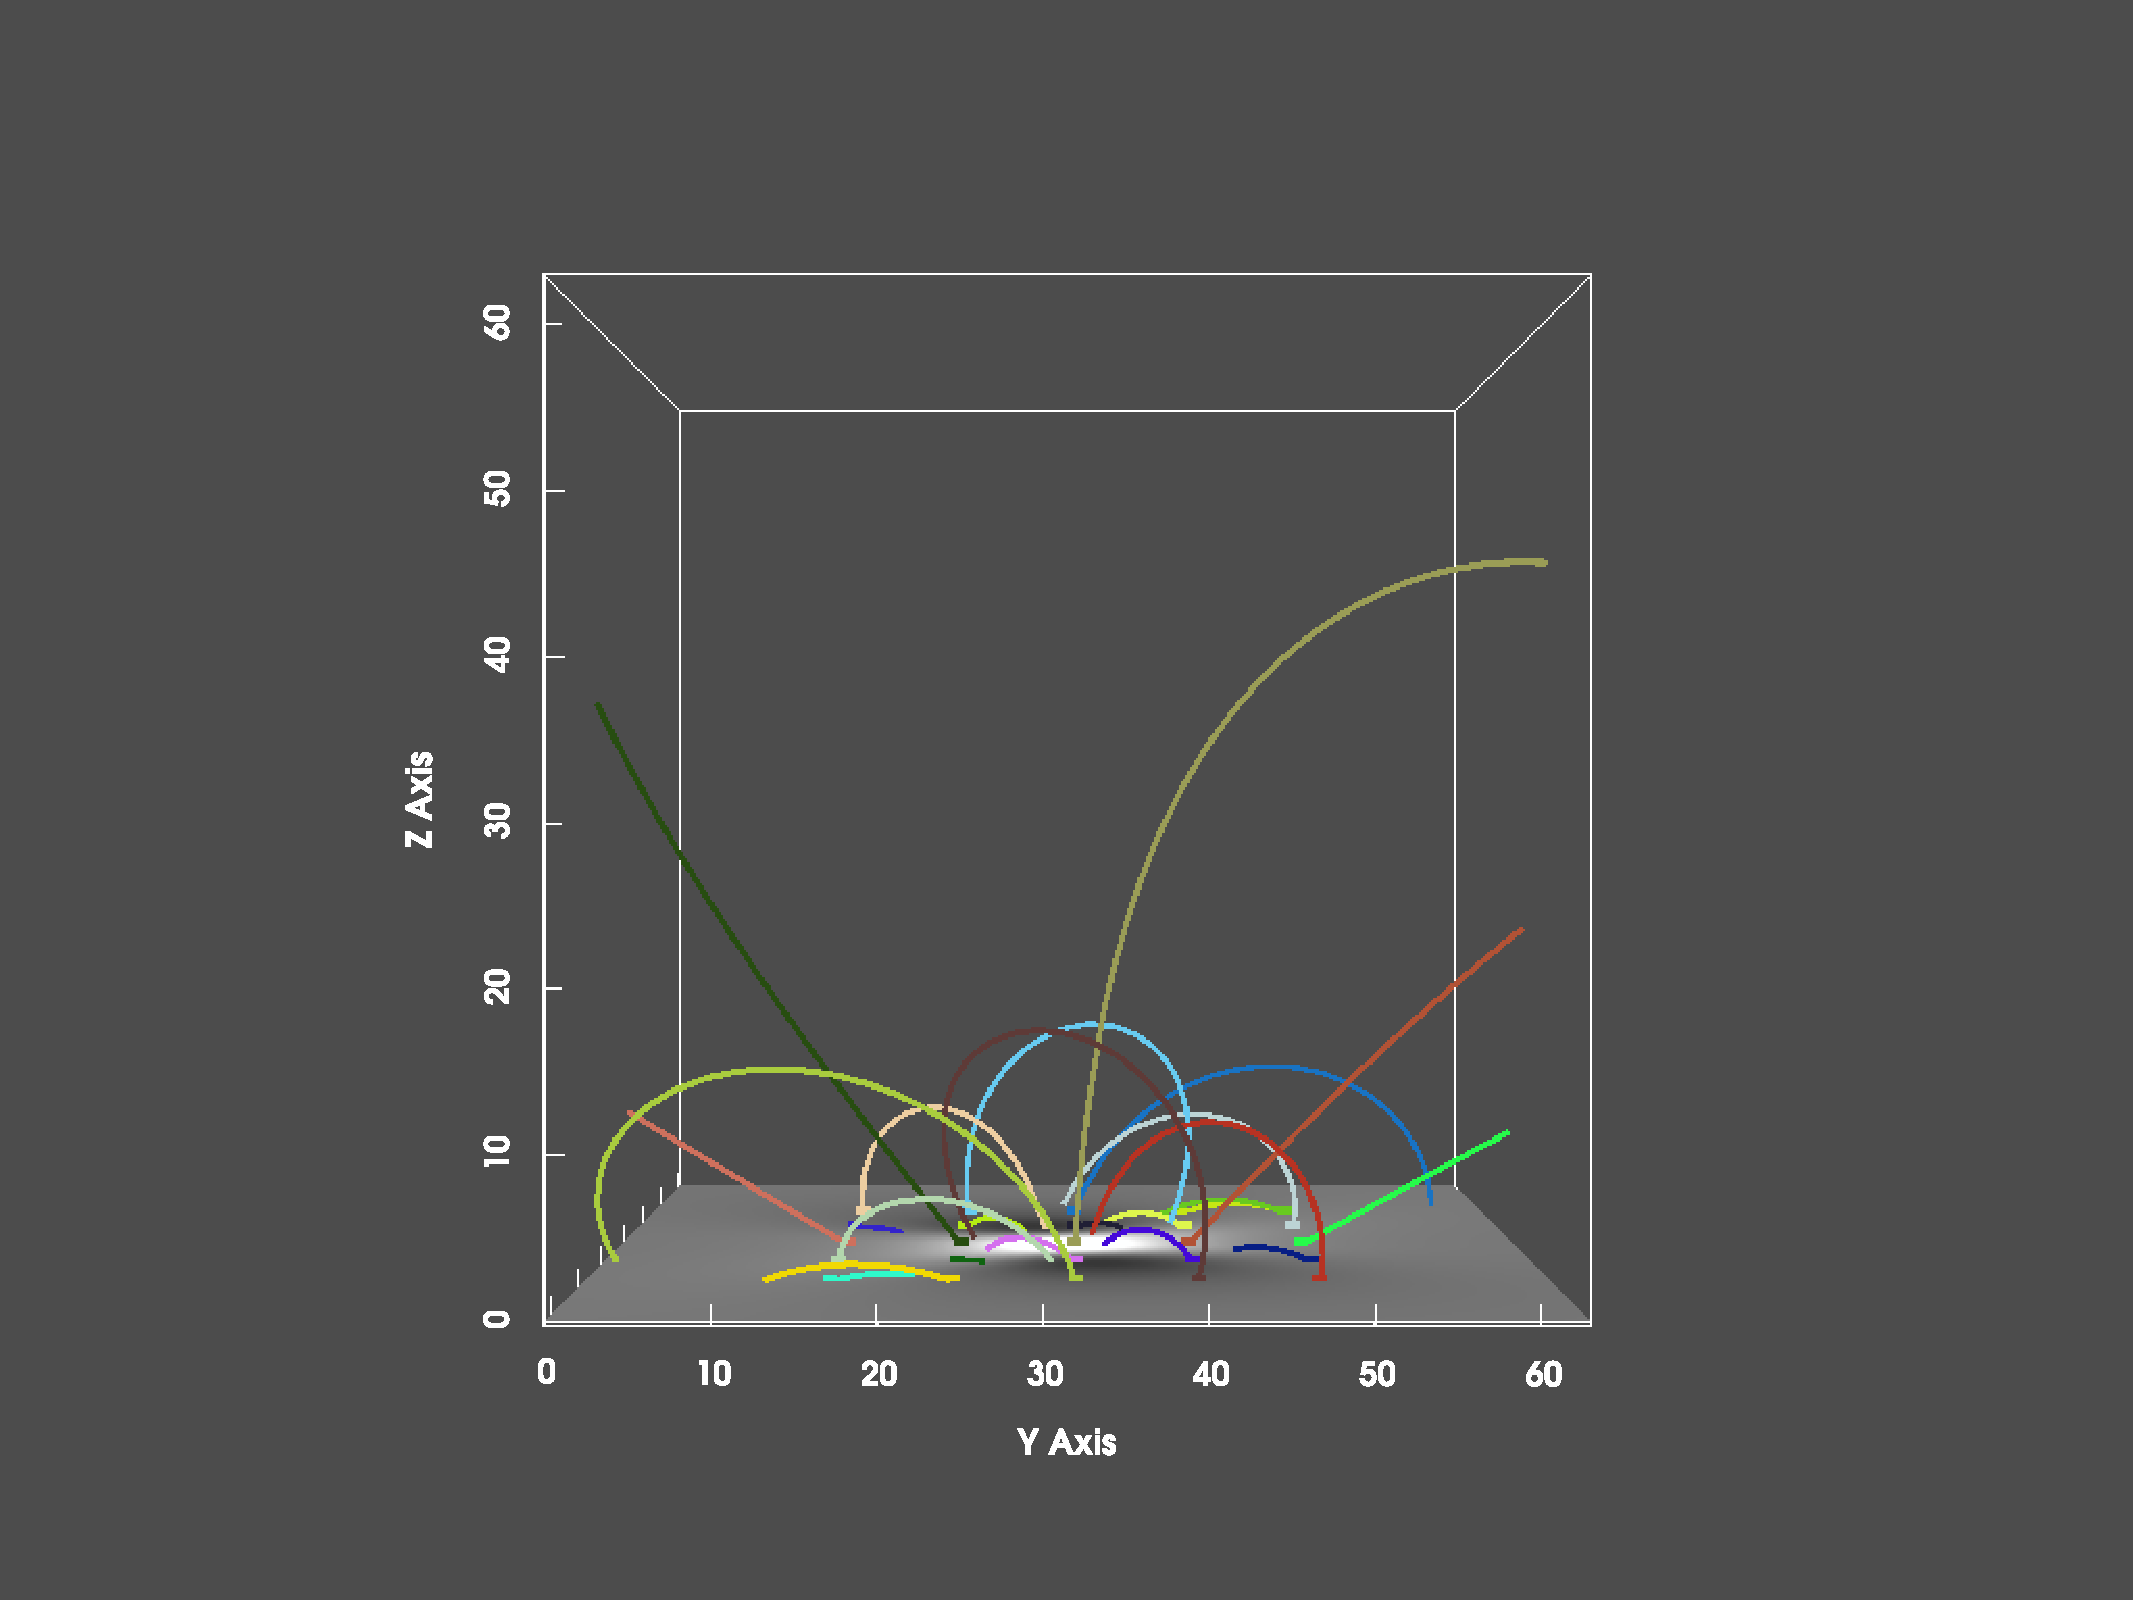
\includegraphics[trim={6cm 1cm 6cm 2cm}, clip, width=\linewidth]{"img/LL_yz.pdf"}
  \end{subfigure}
  
  \caption{The magnetic fields in the yz plane. Each field line is distinguished by its unique color, which is determined by its footpoint at $z=0$ plane.}\label{fig:yz}
\end{figure}

\begin{figure}
  \begin{subfigure}{.5\linewidth}
    \centering
    \caption{PINN(0)}\label{fig:xz0}
    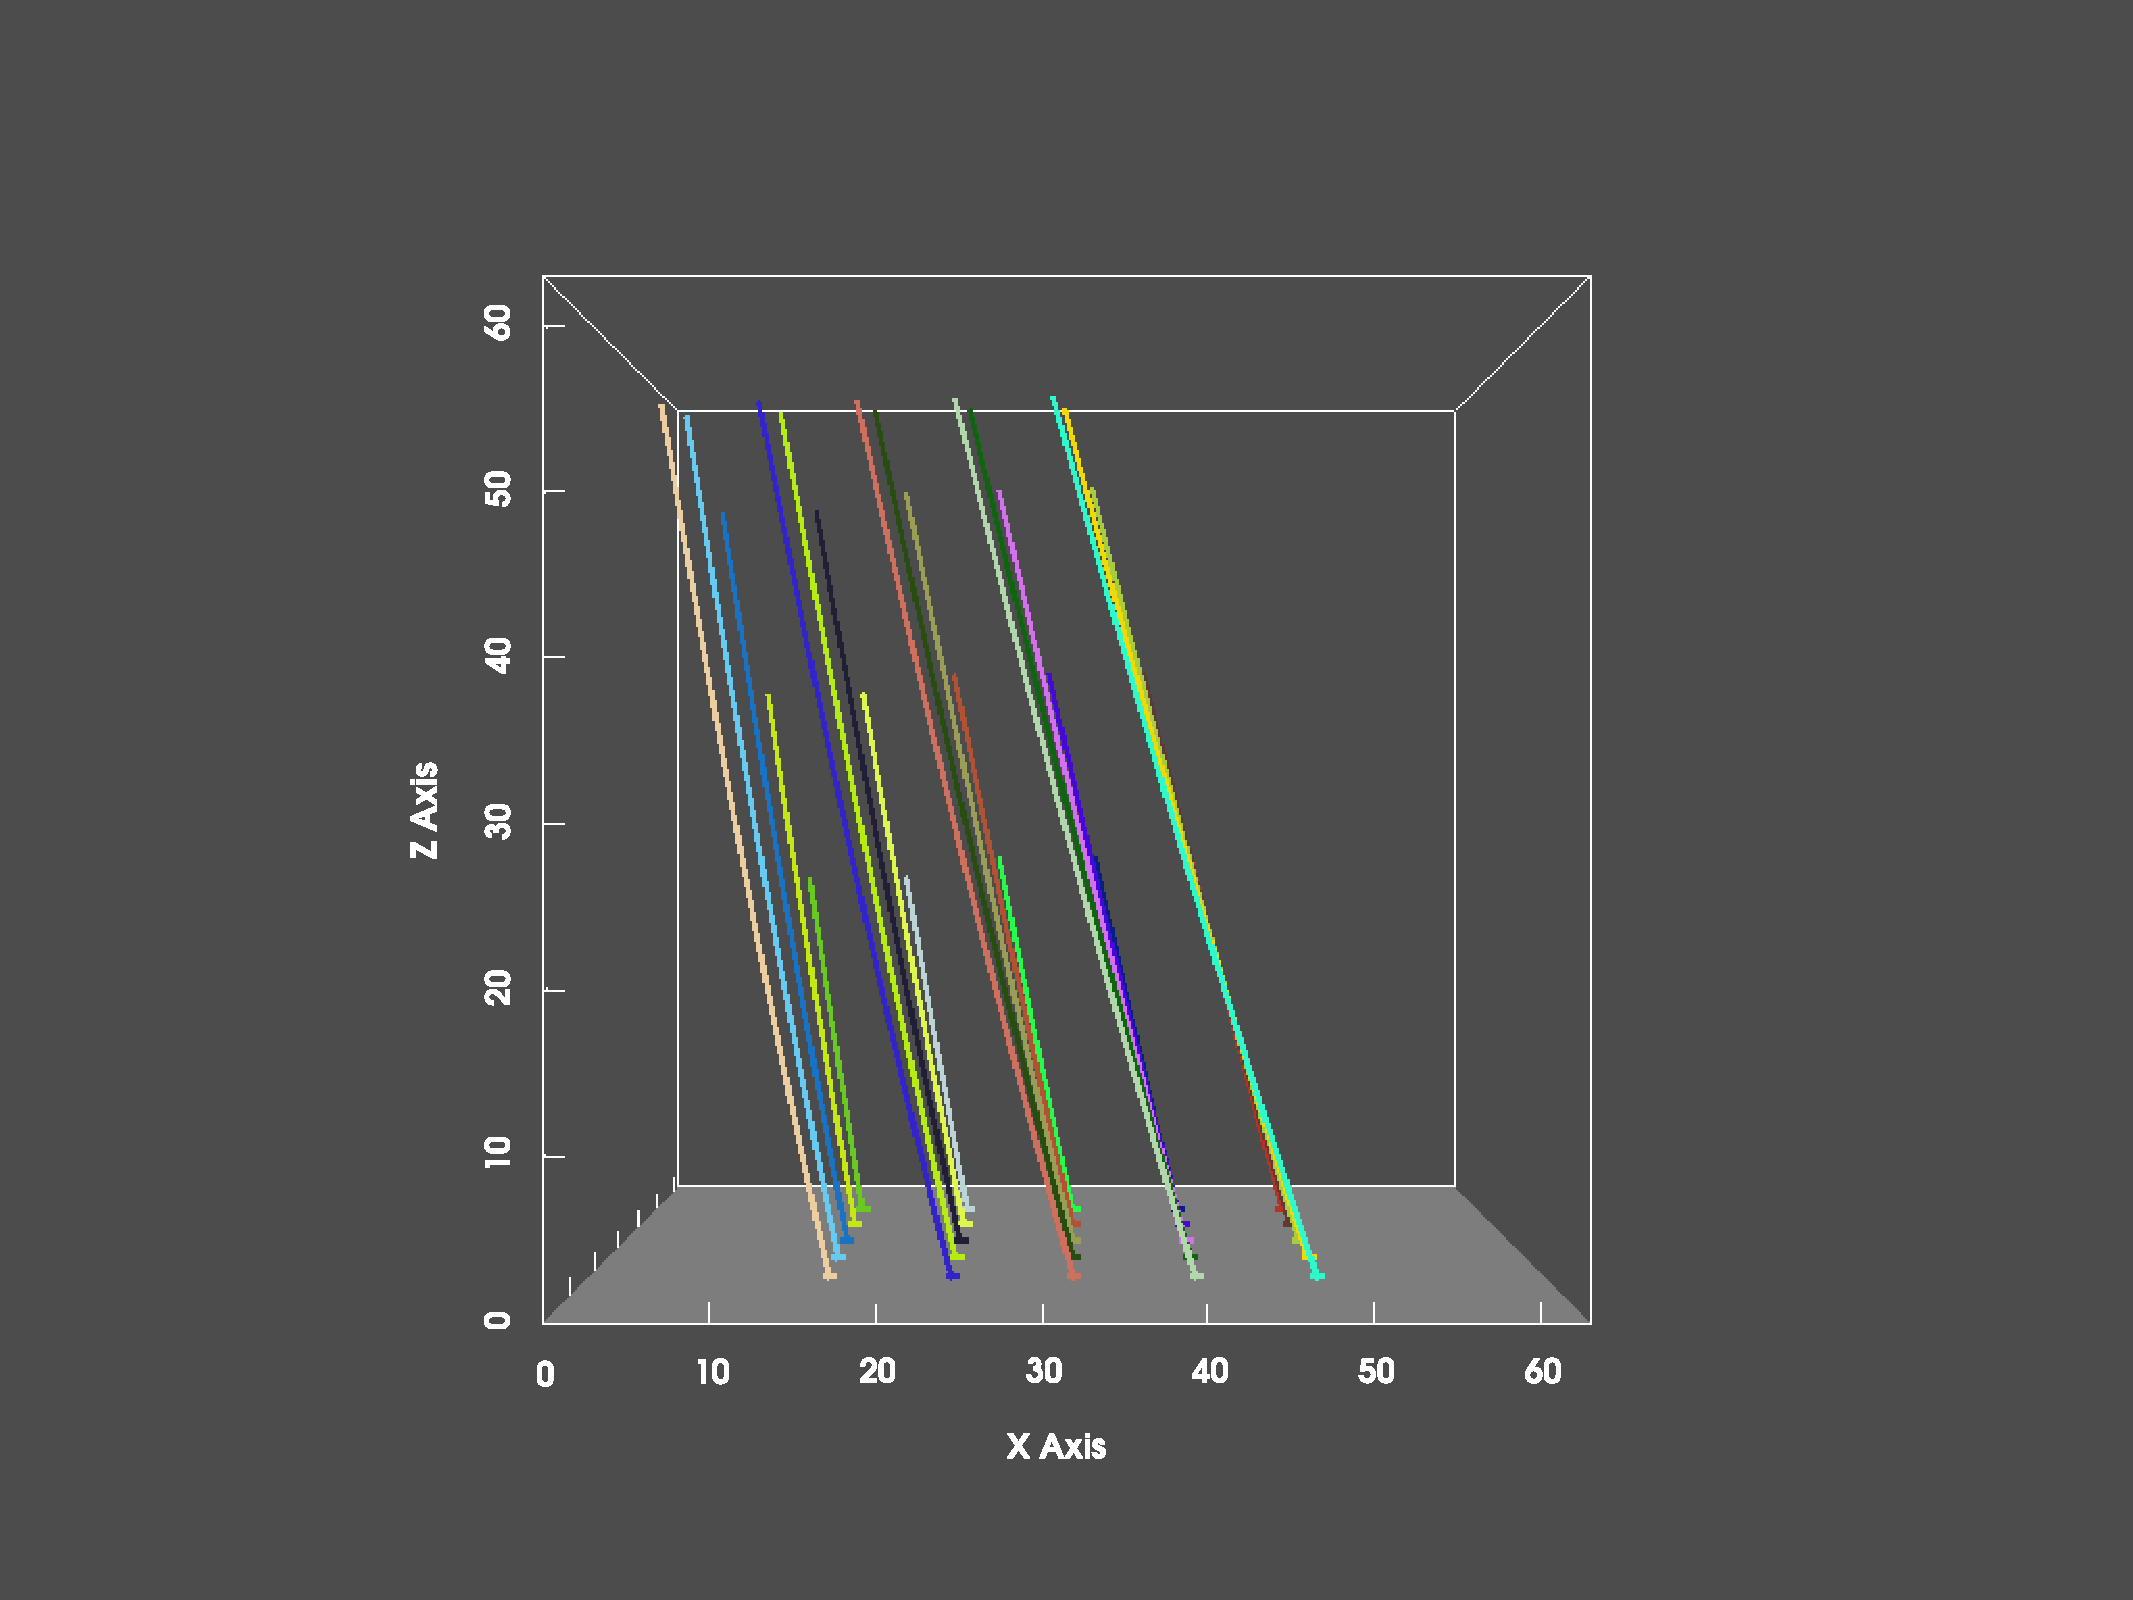
\includegraphics[trim={6cm 1cm 6cm 2cm}, clip, width=\linewidth]{"img/PINN_000000_xz.pdf"}
  \end{subfigure}%
  \begin{subfigure}{.5\linewidth}
    \centering
    \caption{PINN(100)}
    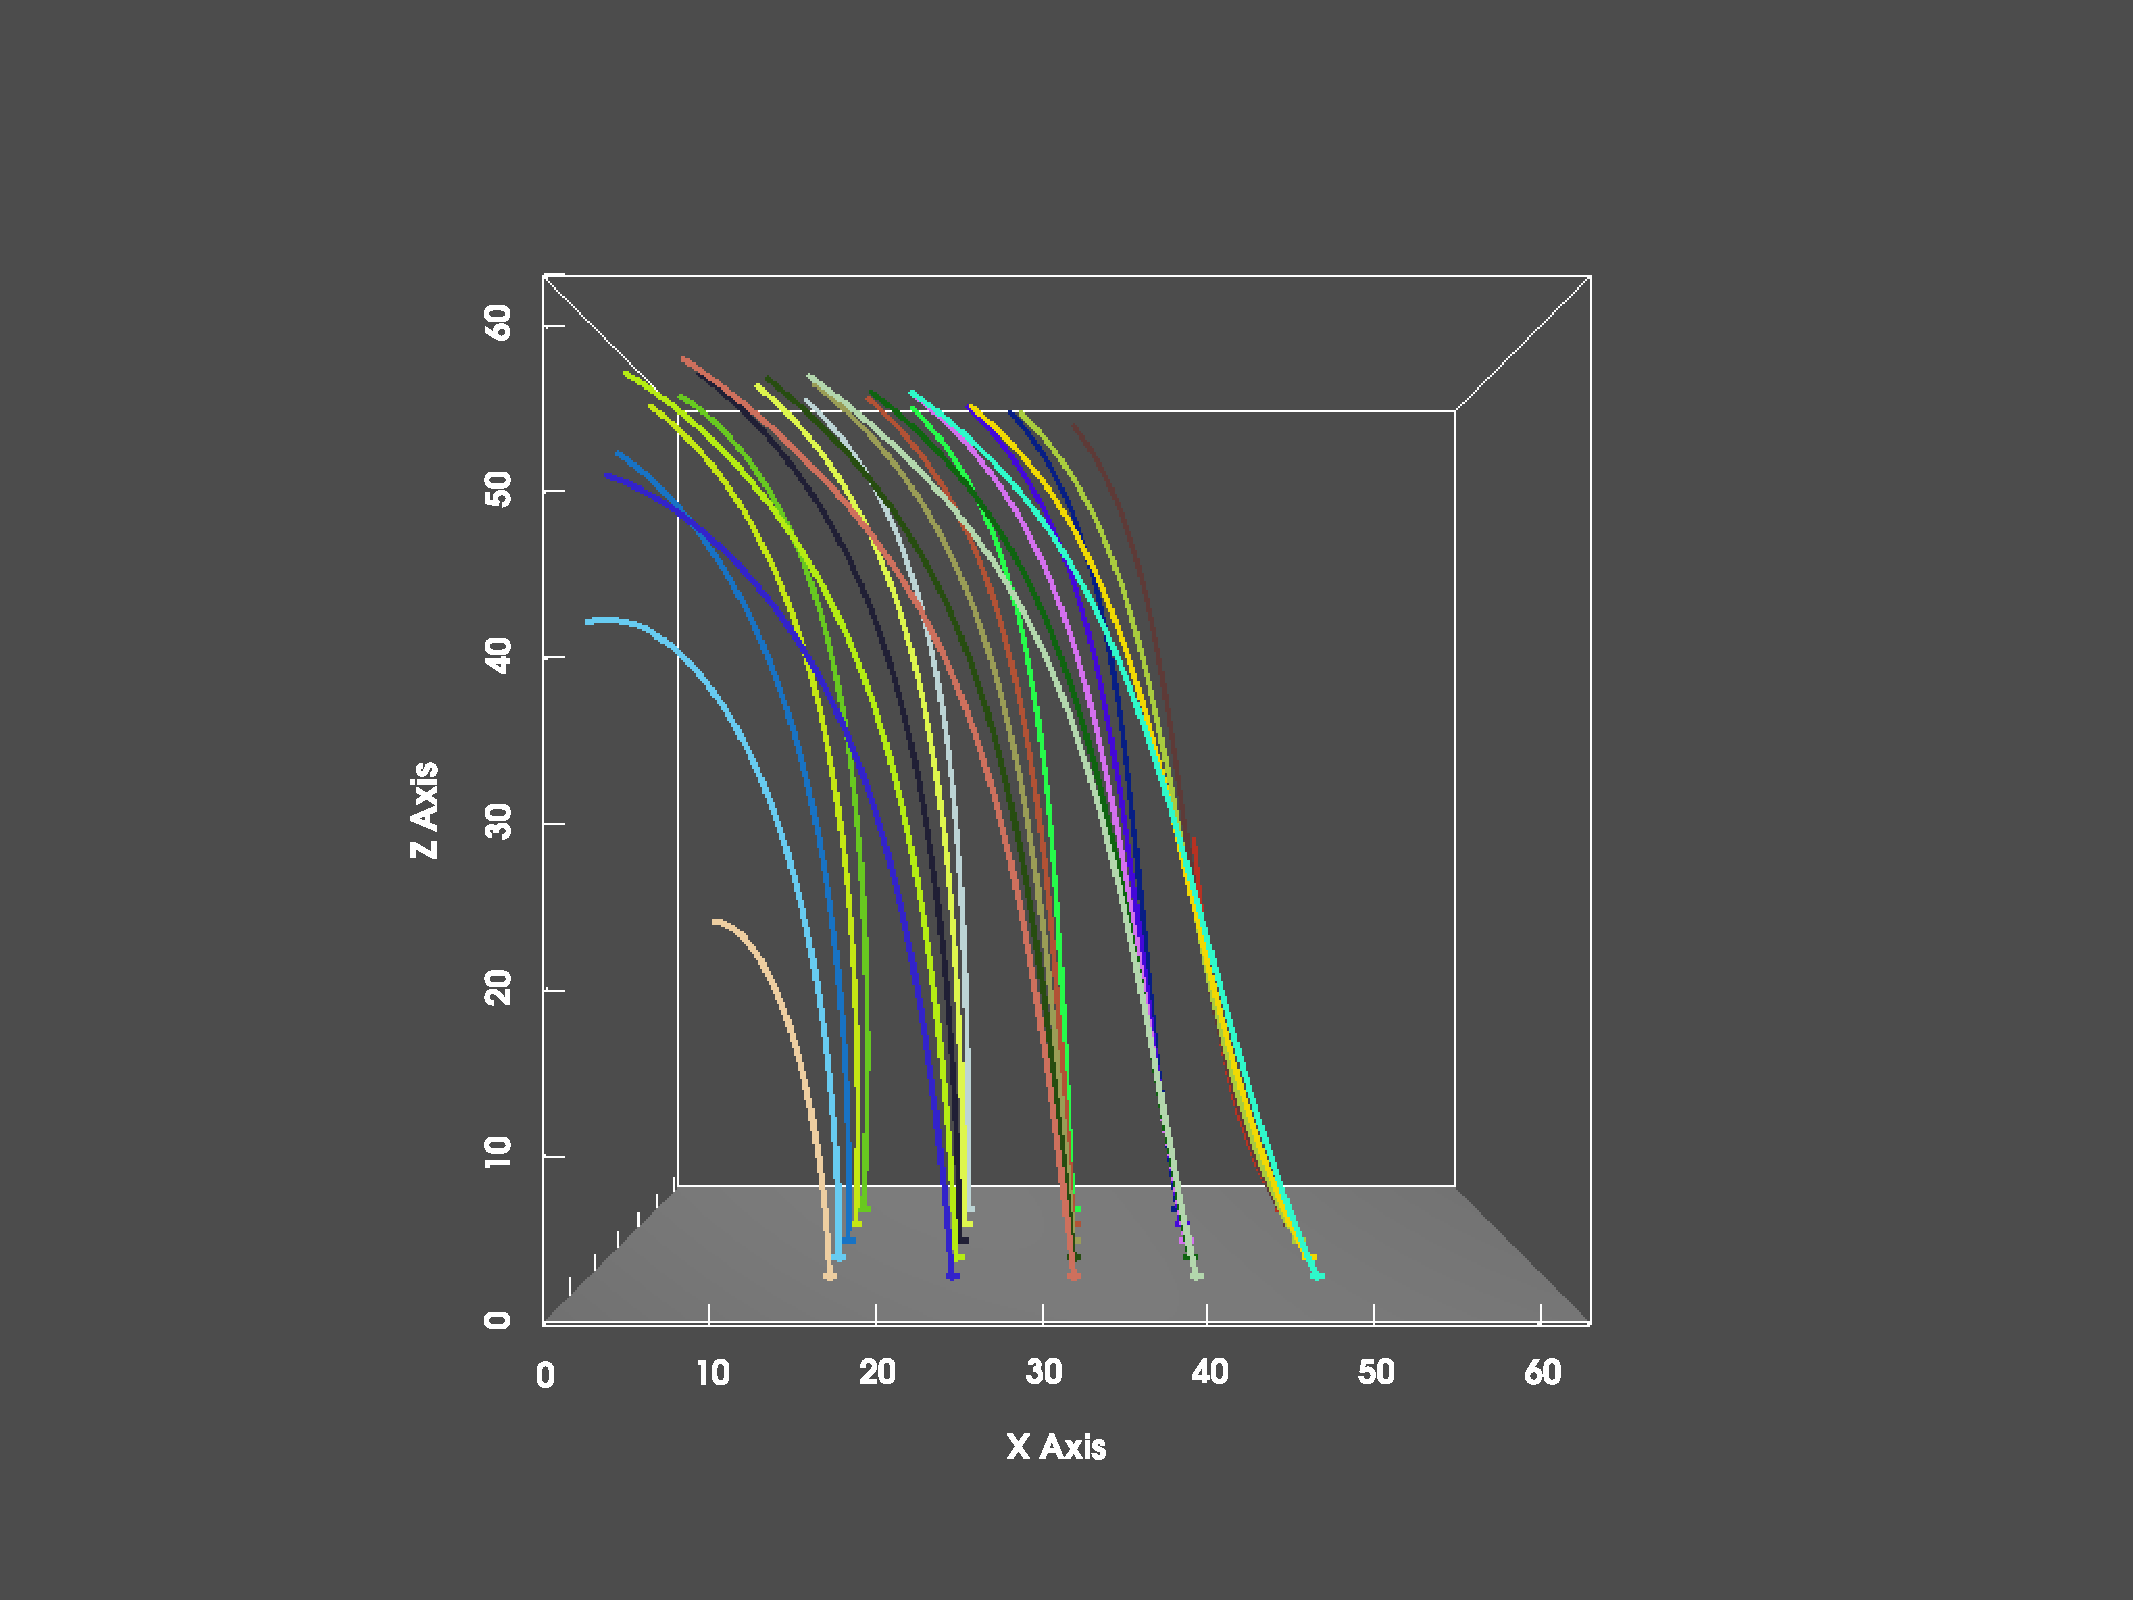
\includegraphics[trim={6cm 1cm 6cm 2cm}, clip, width=\linewidth]{"img/PINN_000100_xz.pdf"}
  \end{subfigure}

  \begin{subfigure}{.5\linewidth}
    \centering
    \caption{PINN(1000)}
    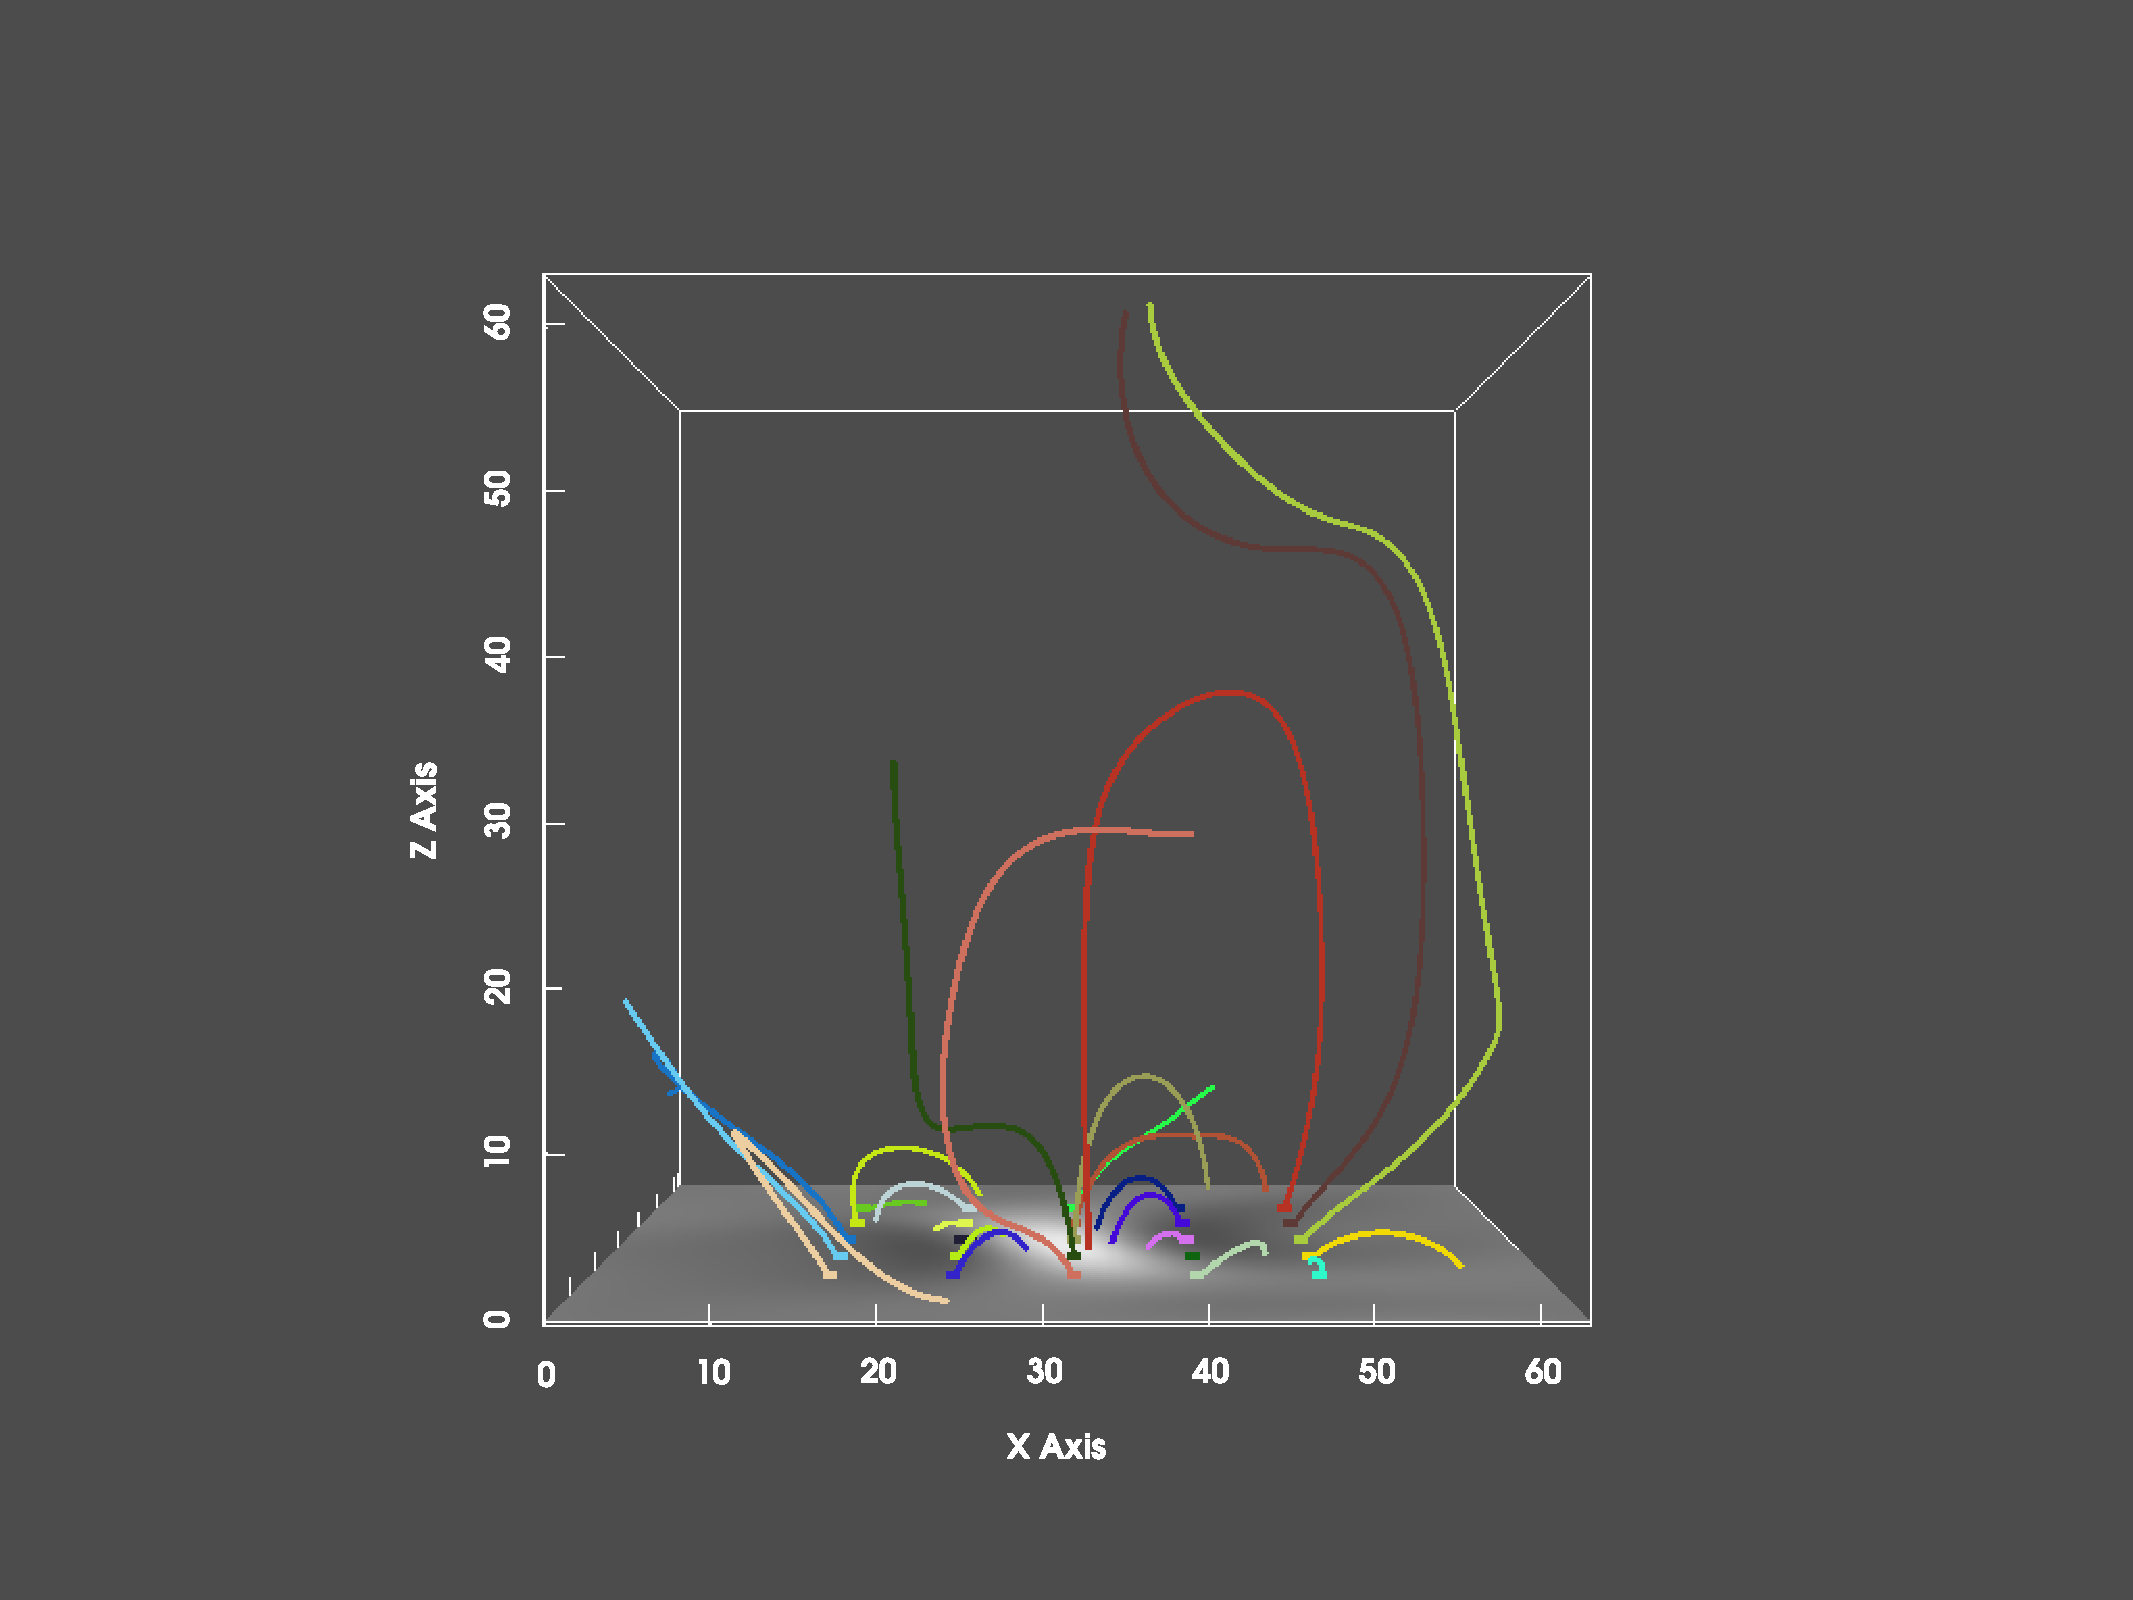
\includegraphics[trim={6cm 1cm 6cm 2cm}, clip, width=\linewidth]{"img/PINN_001000_xz.pdf"}
  \end{subfigure}%
  \begin{subfigure}{.5\linewidth}
    \centering
    \caption{PINN(10000)}
    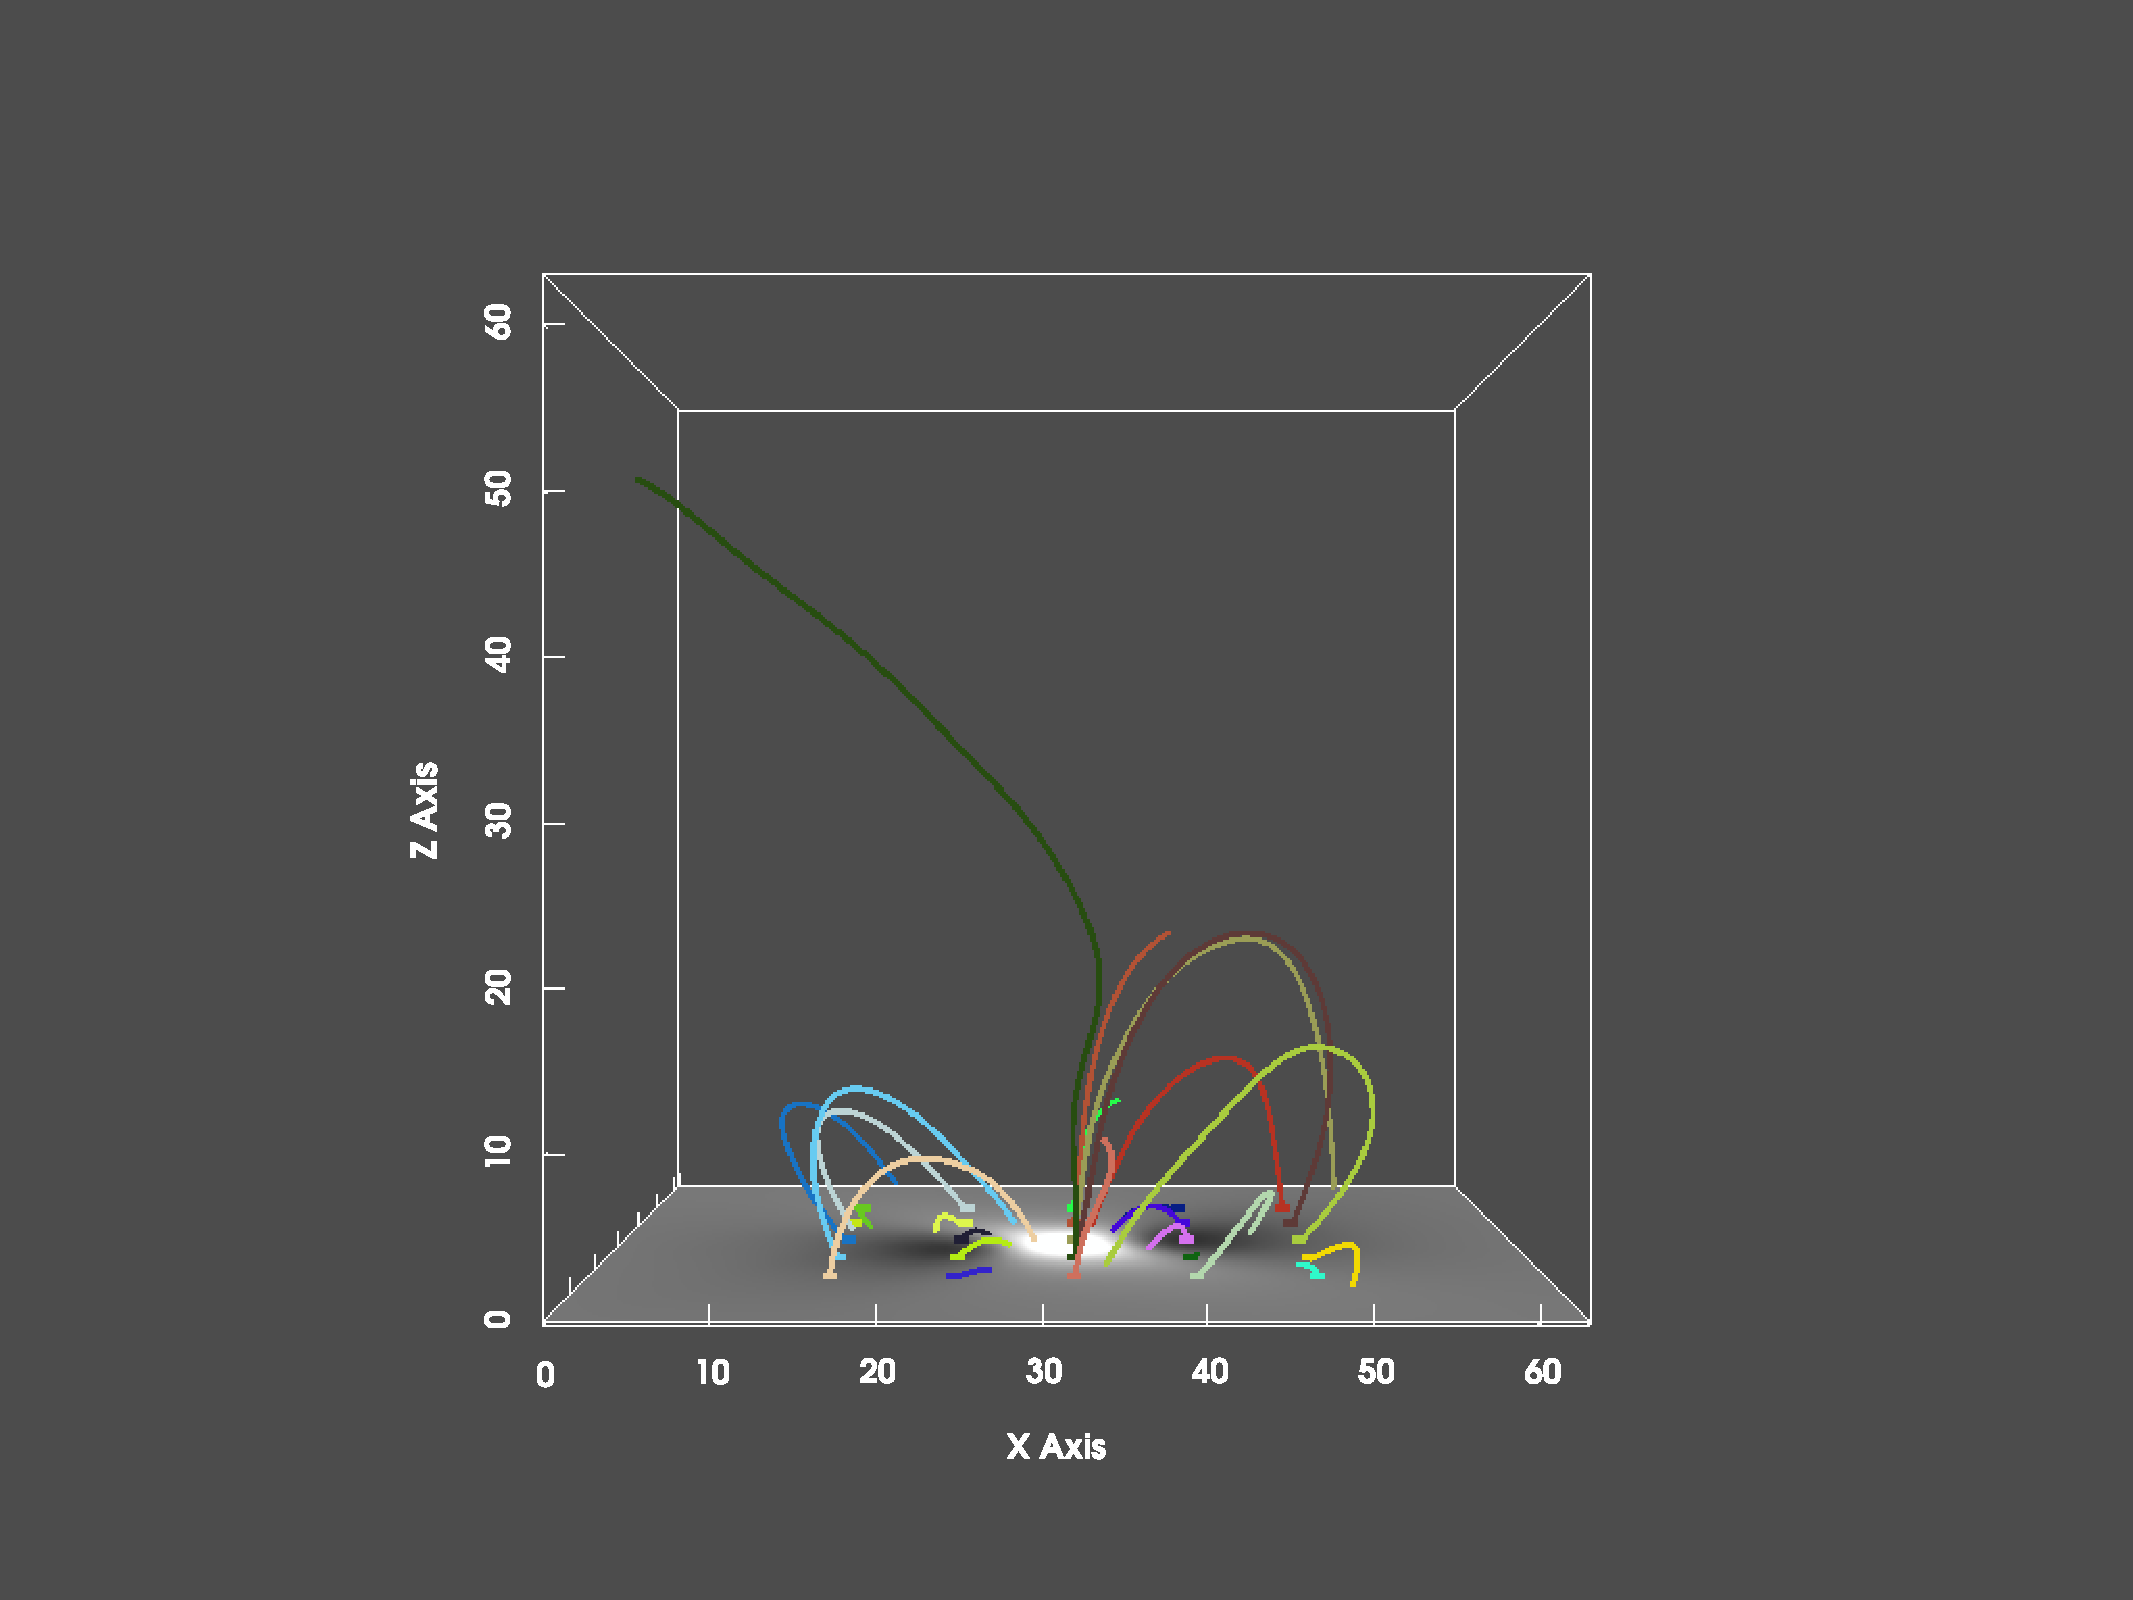
\includegraphics[trim={6cm 1cm 6cm 2cm}, clip, width=\linewidth]{"img/PINN_010000_xz.pdf"}
  \end{subfigure}

  \begin{subfigure}{.5\linewidth}
    \centering
    \caption{PINN(25000)}
    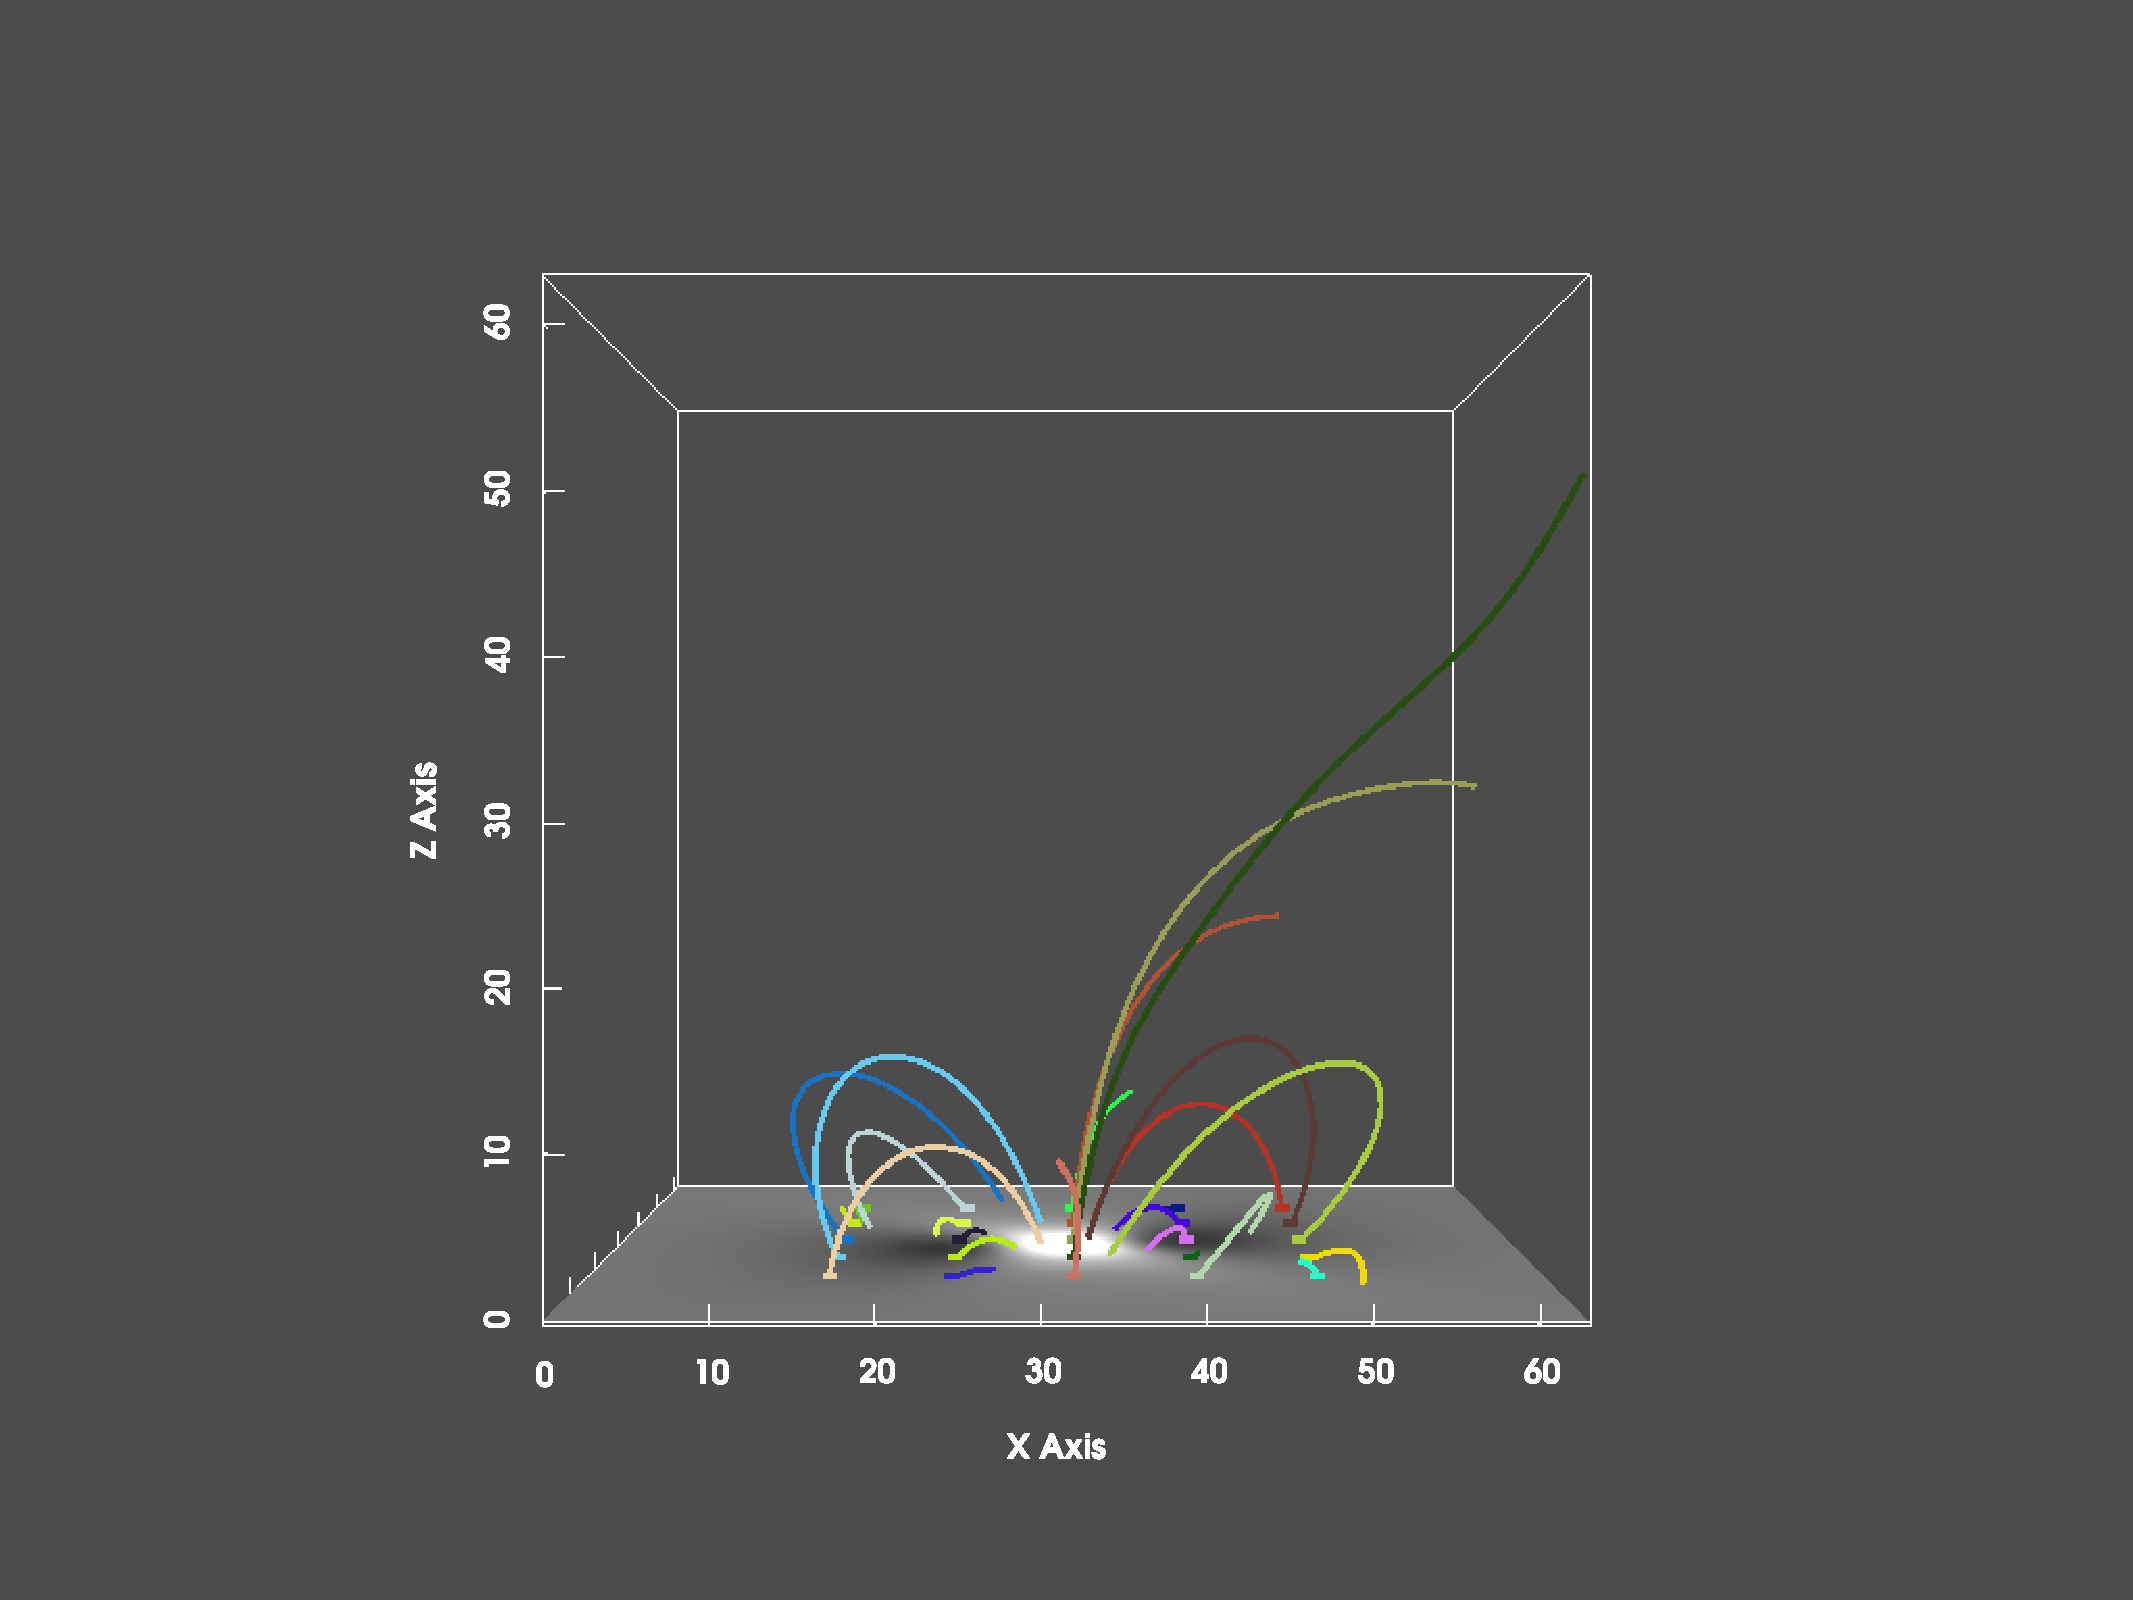
\includegraphics[trim={6cm 1cm 6cm 2cm}, clip, width=\linewidth]{"img/PINN_025000_xz.pdf"}
  \end{subfigure}%
  \begin{subfigure}{.5\linewidth}
    \centering
    \caption{PINN(50000)}
    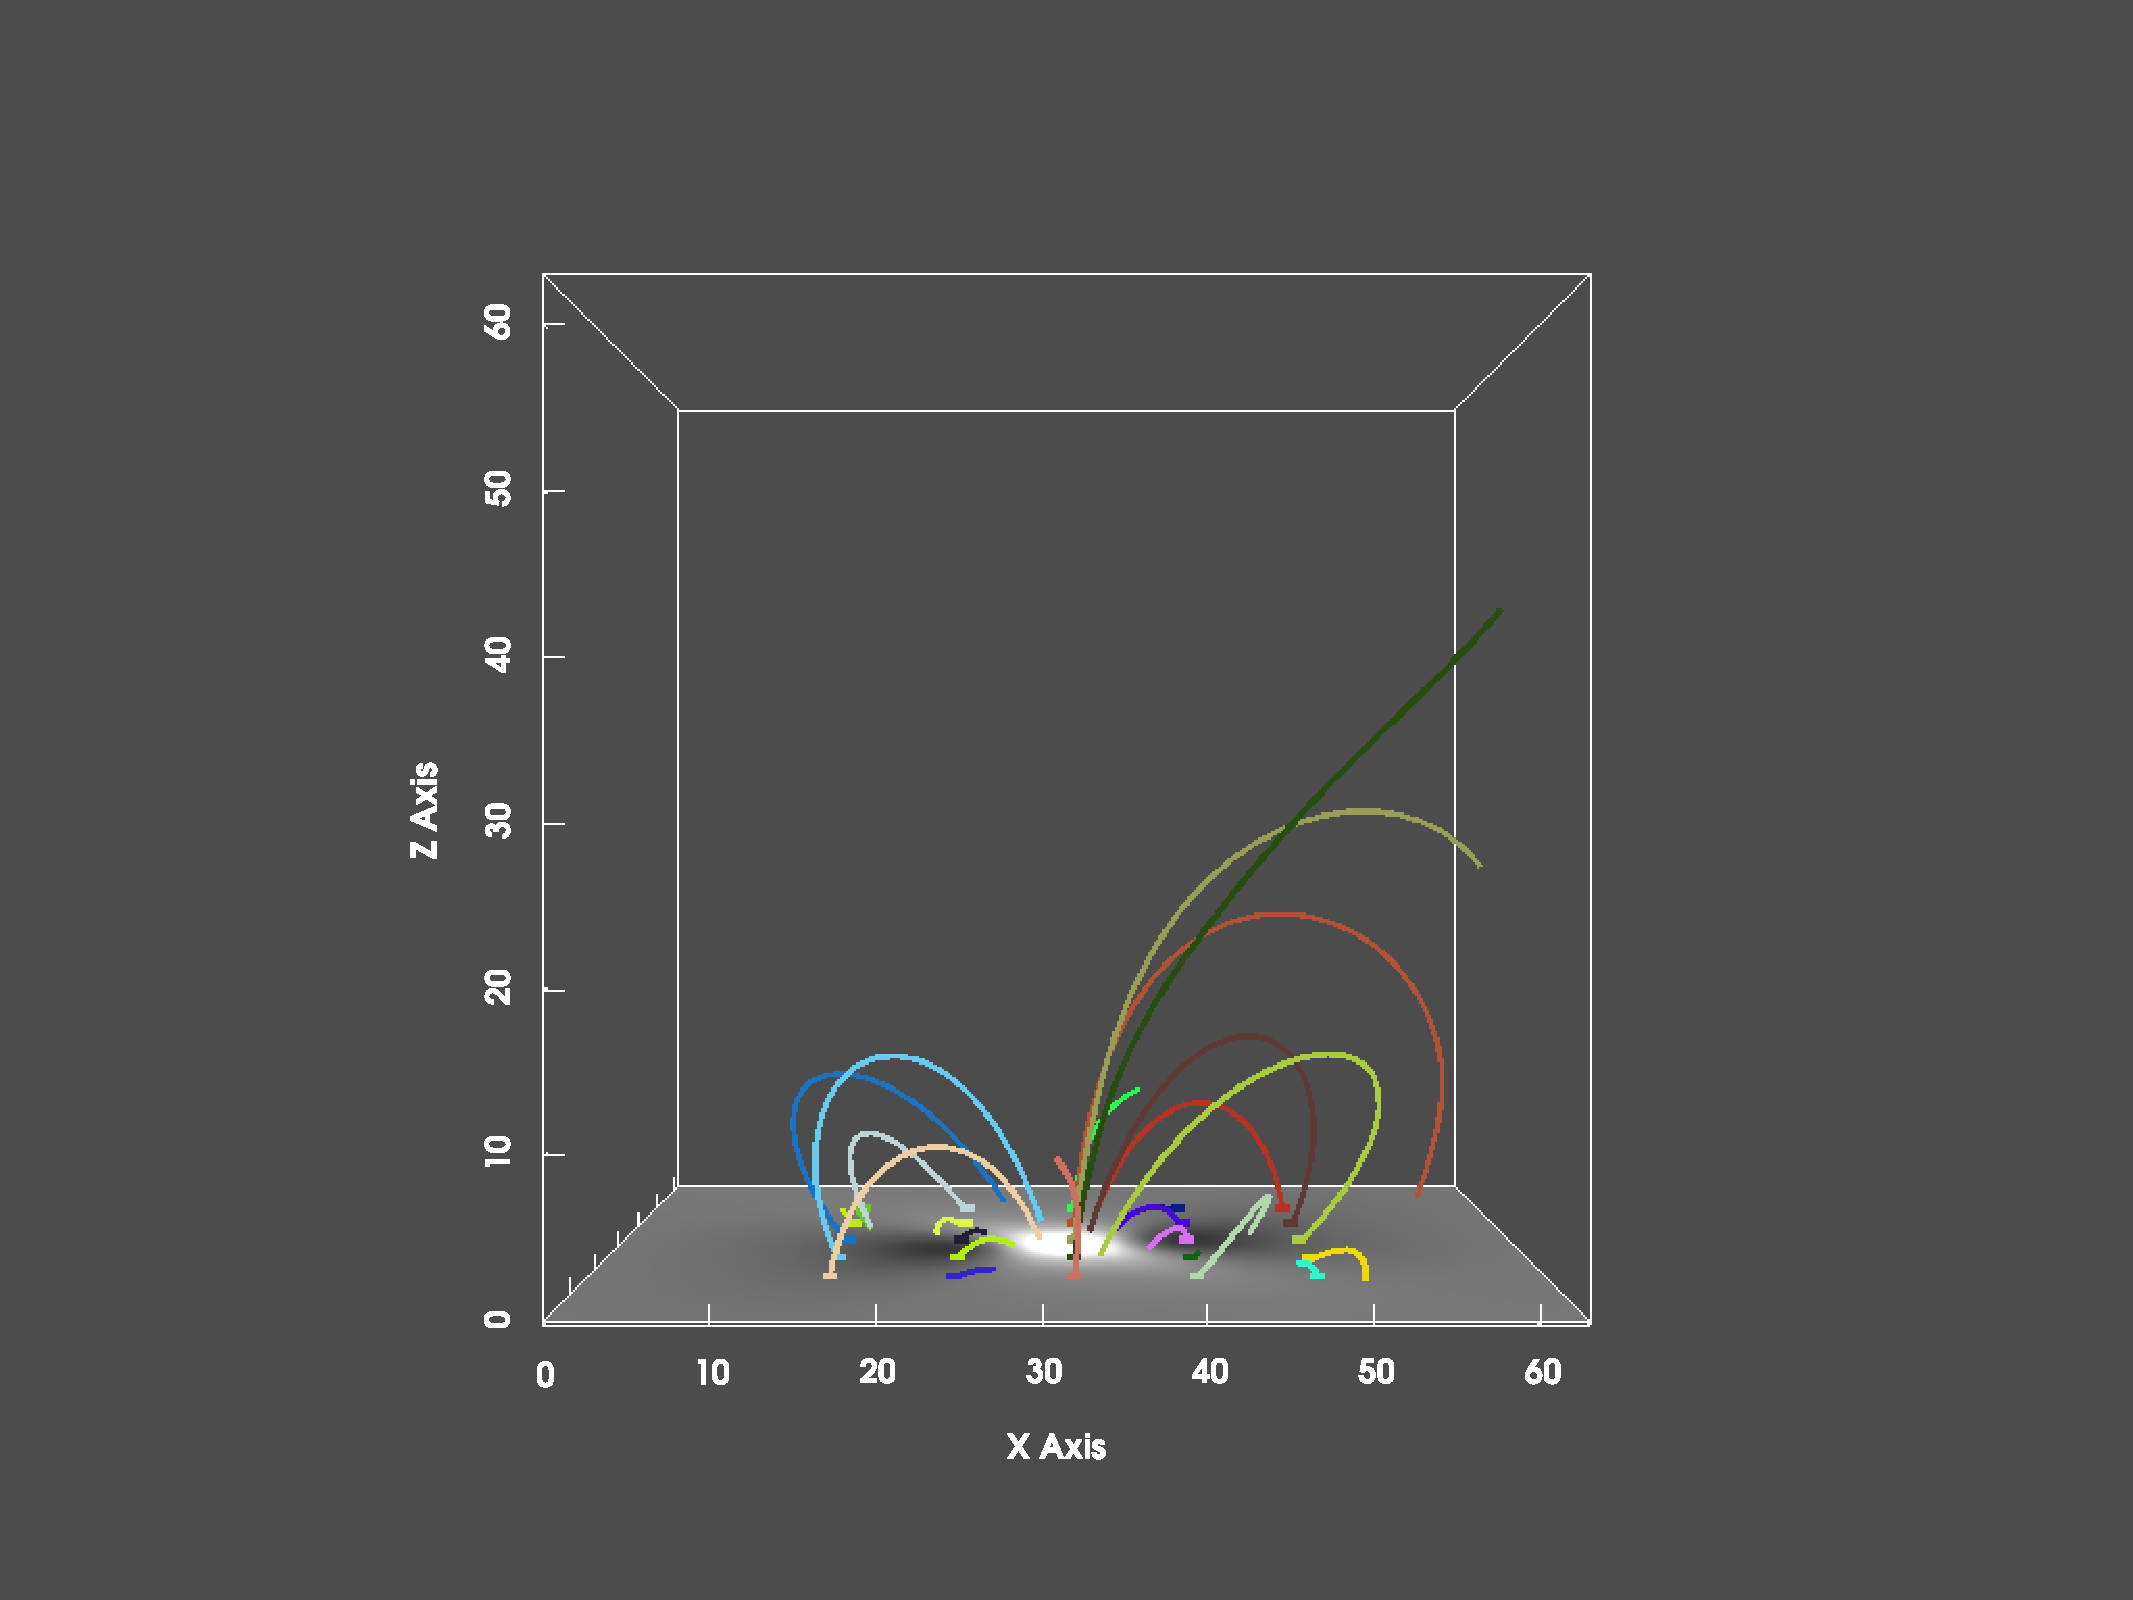
\includegraphics[trim={6cm 1cm 6cm 2cm}, clip, width=\linewidth]{"img/PINN_050000_xz.pdf"}
  \end{subfigure}
  
  \begin{subfigure}{.5\linewidth}
    \centering
    \caption{Potential}
    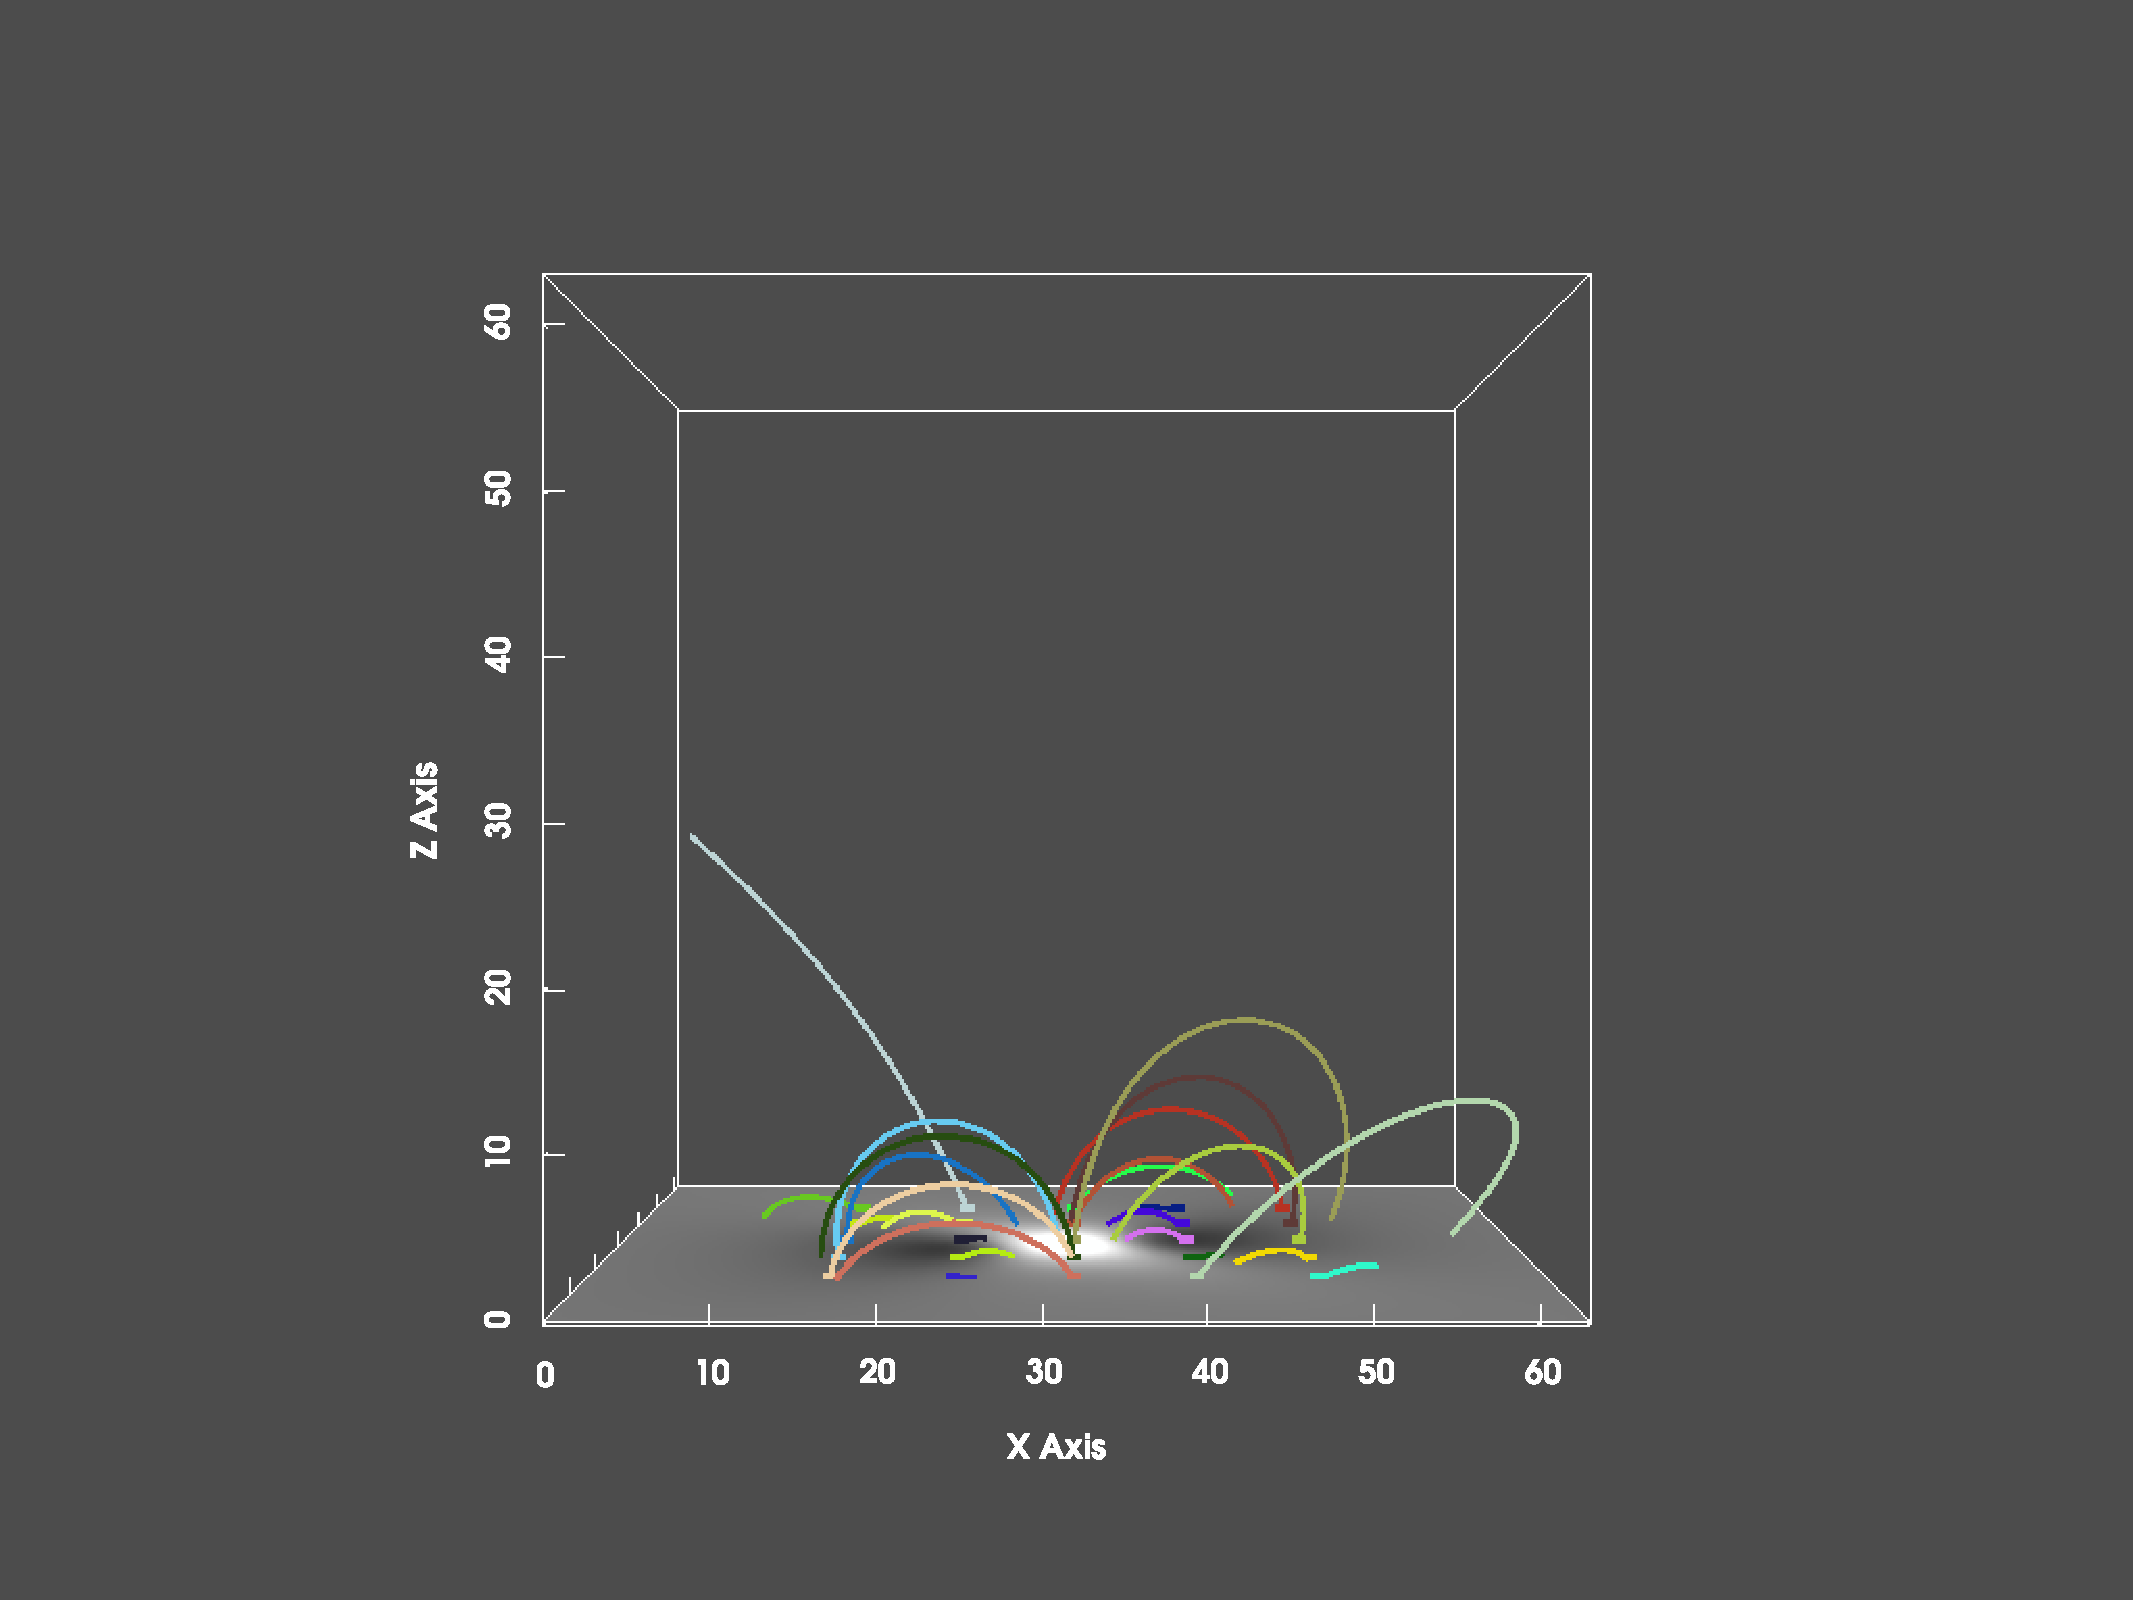
\includegraphics[trim={6cm 1cm 6cm 2cm}, clip, width=\linewidth]{"img/LL_pot_xz.pdf"}
  \end{subfigure}%
  \begin{subfigure}{.5\linewidth}
    \centering
    \caption{Low-Lou}
    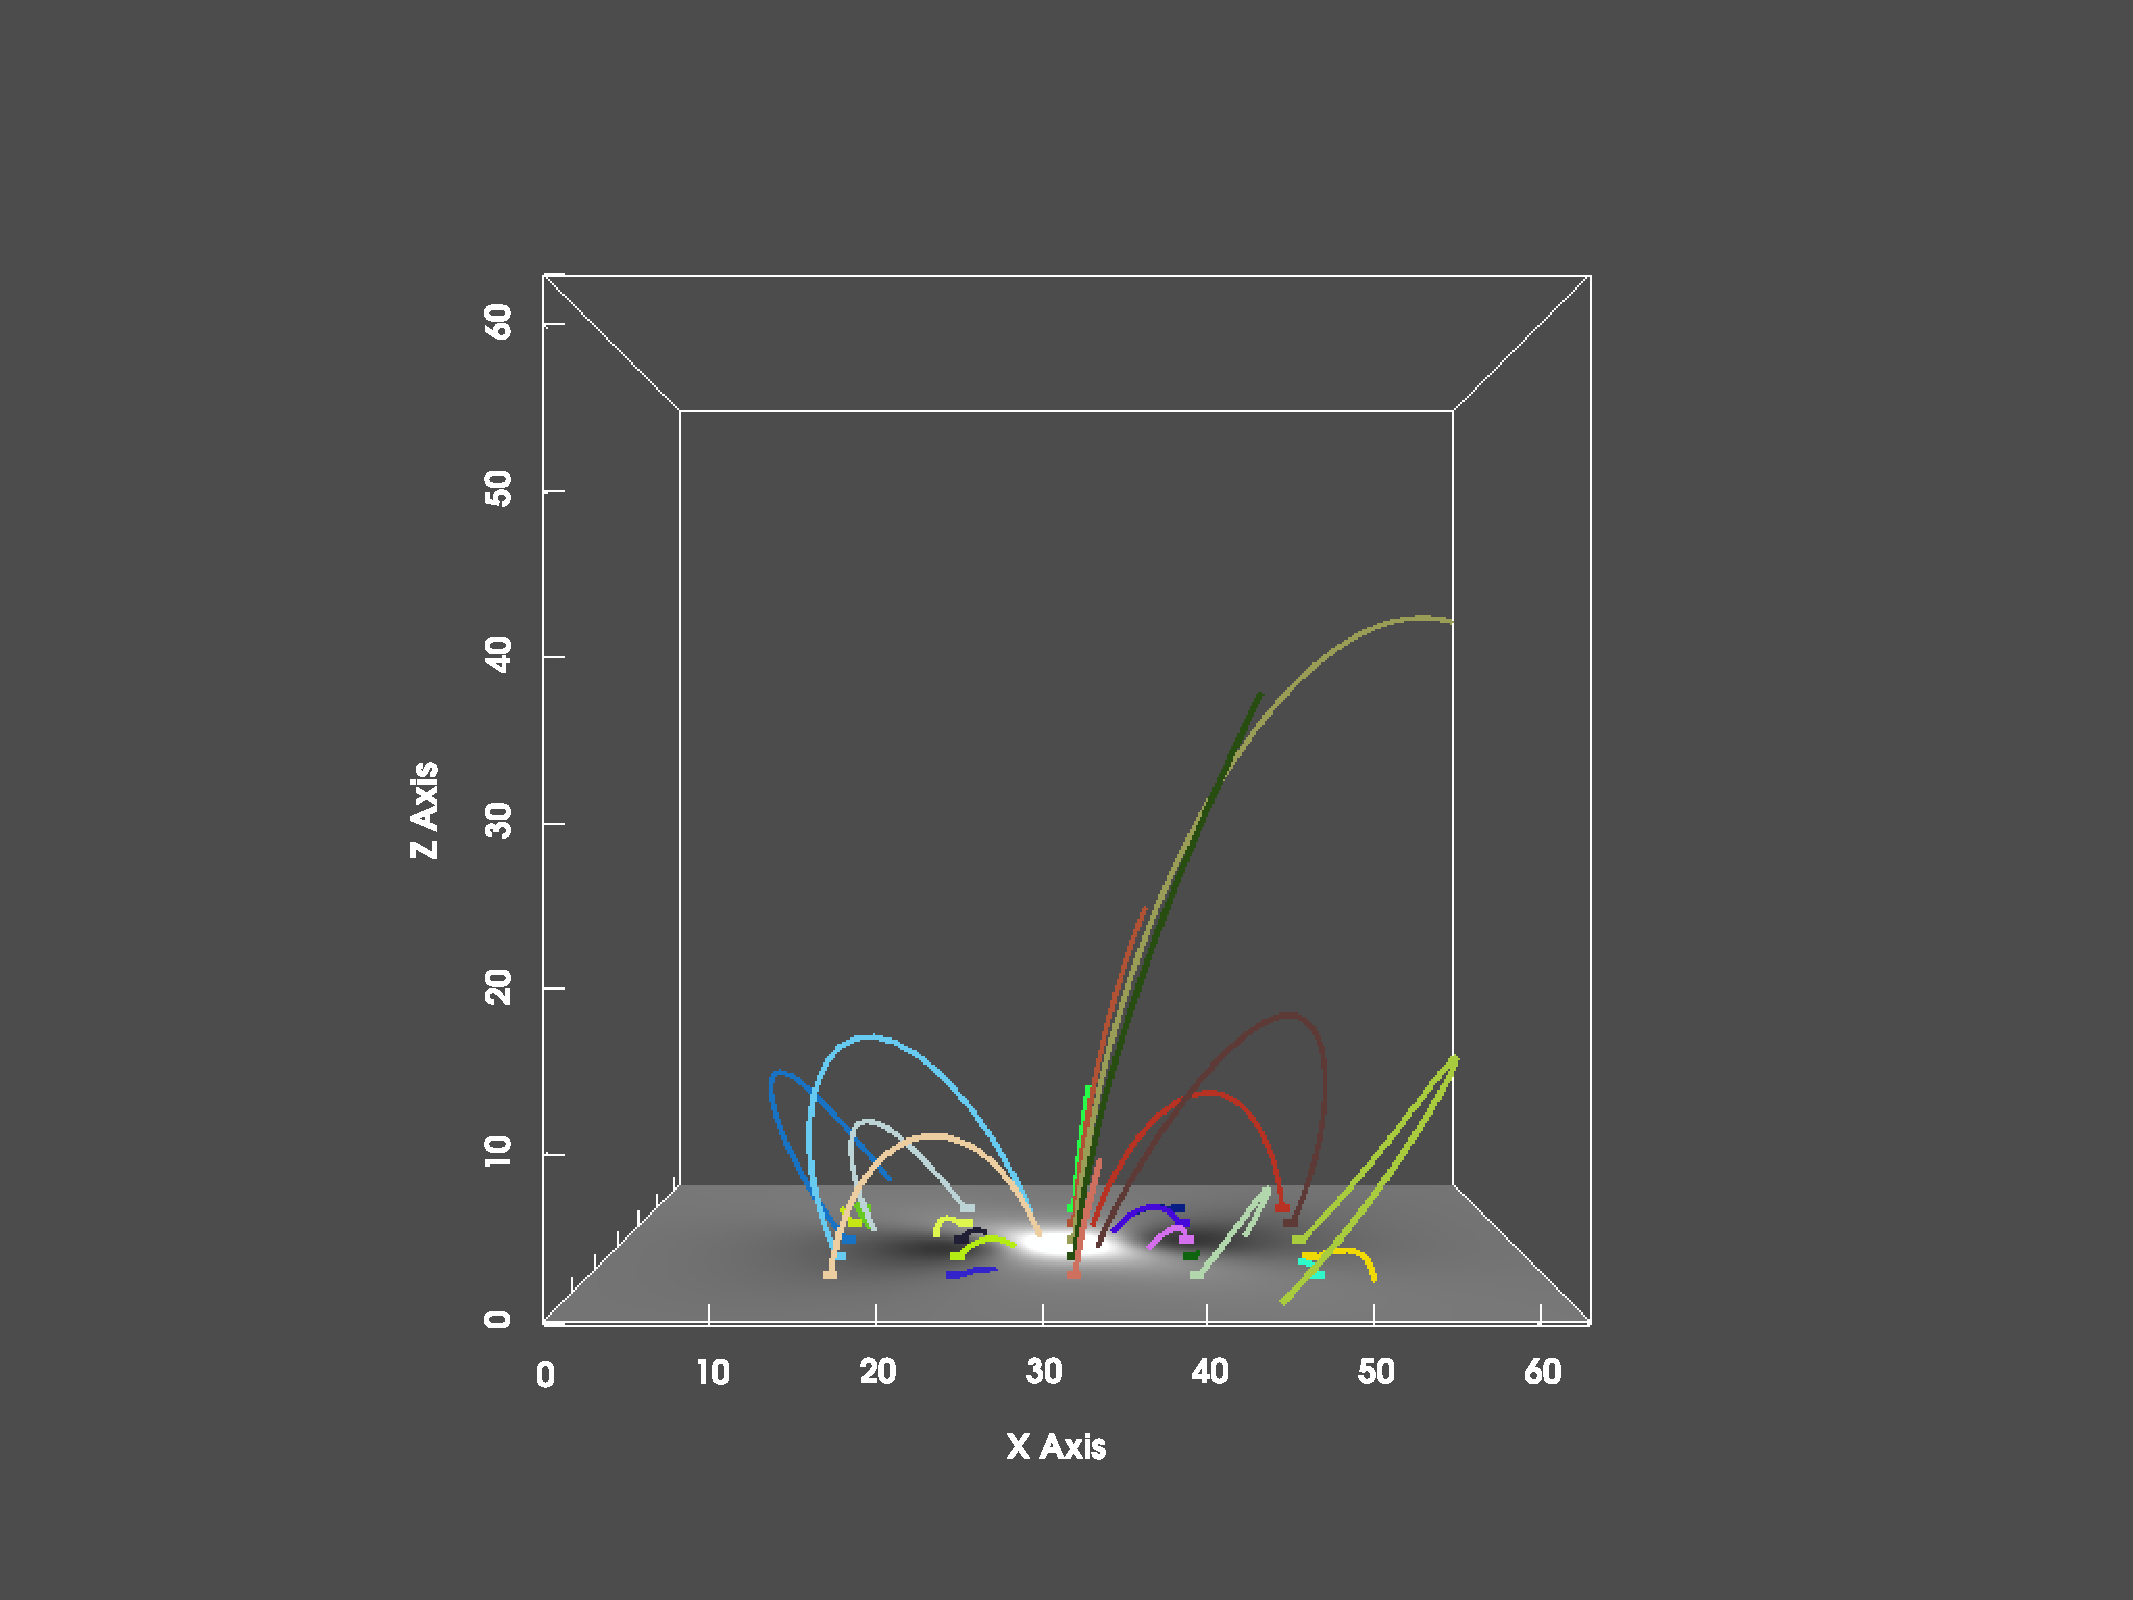
\includegraphics[trim={6cm 1cm 6cm 2cm}, clip, width=\linewidth]{"img/LL_xz.pdf"}
  \end{subfigure}
  
  \caption{The magnetic fields in the xz plane. Each field line is distinguished by its unique color, which is determined by its footpoint at $z=0$ plane.}\label{fig:xz}
\end{figure}


\begin{figure}
  \begin{subfigure}{.5\linewidth}
    \centering
    \caption{PINN(0)}\label{fig:pv0}
    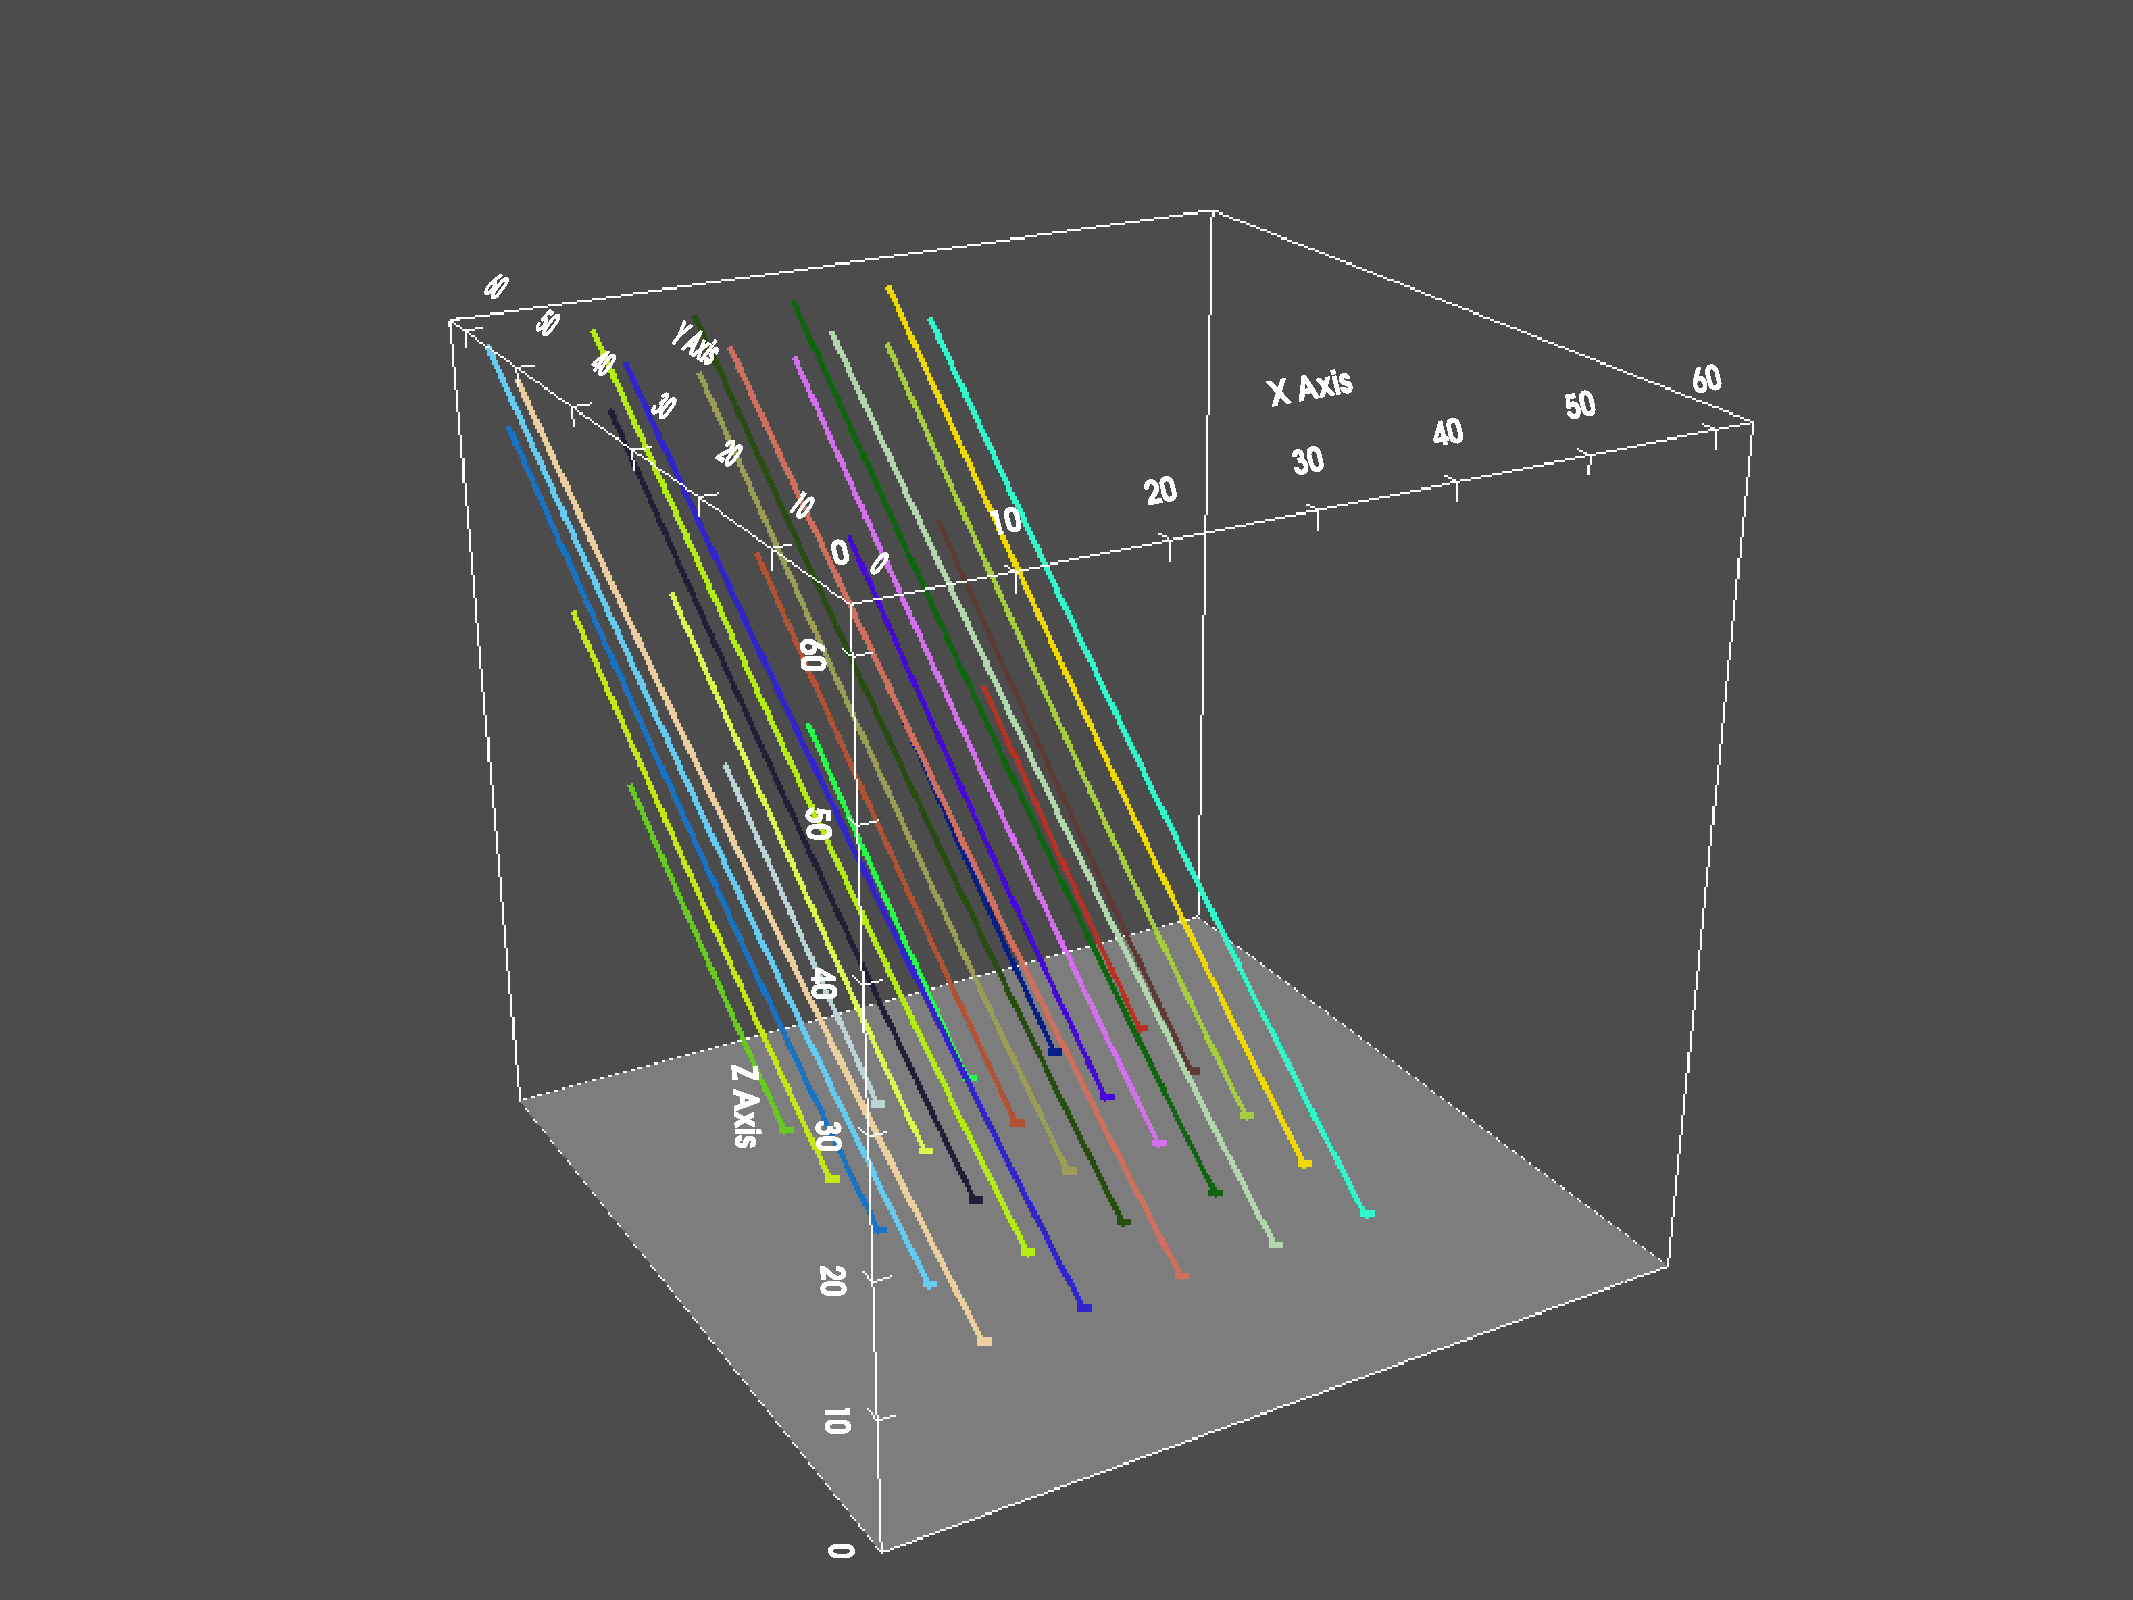
\includegraphics[trim={6cm 0cm 6cm 3cm}, clip, width=\linewidth]{"img/PINN_000000_xz_tilted.pdf"}
  \end{subfigure}%
  \begin{subfigure}{.5\linewidth}
    \centering
    \caption{PINN(100)}
    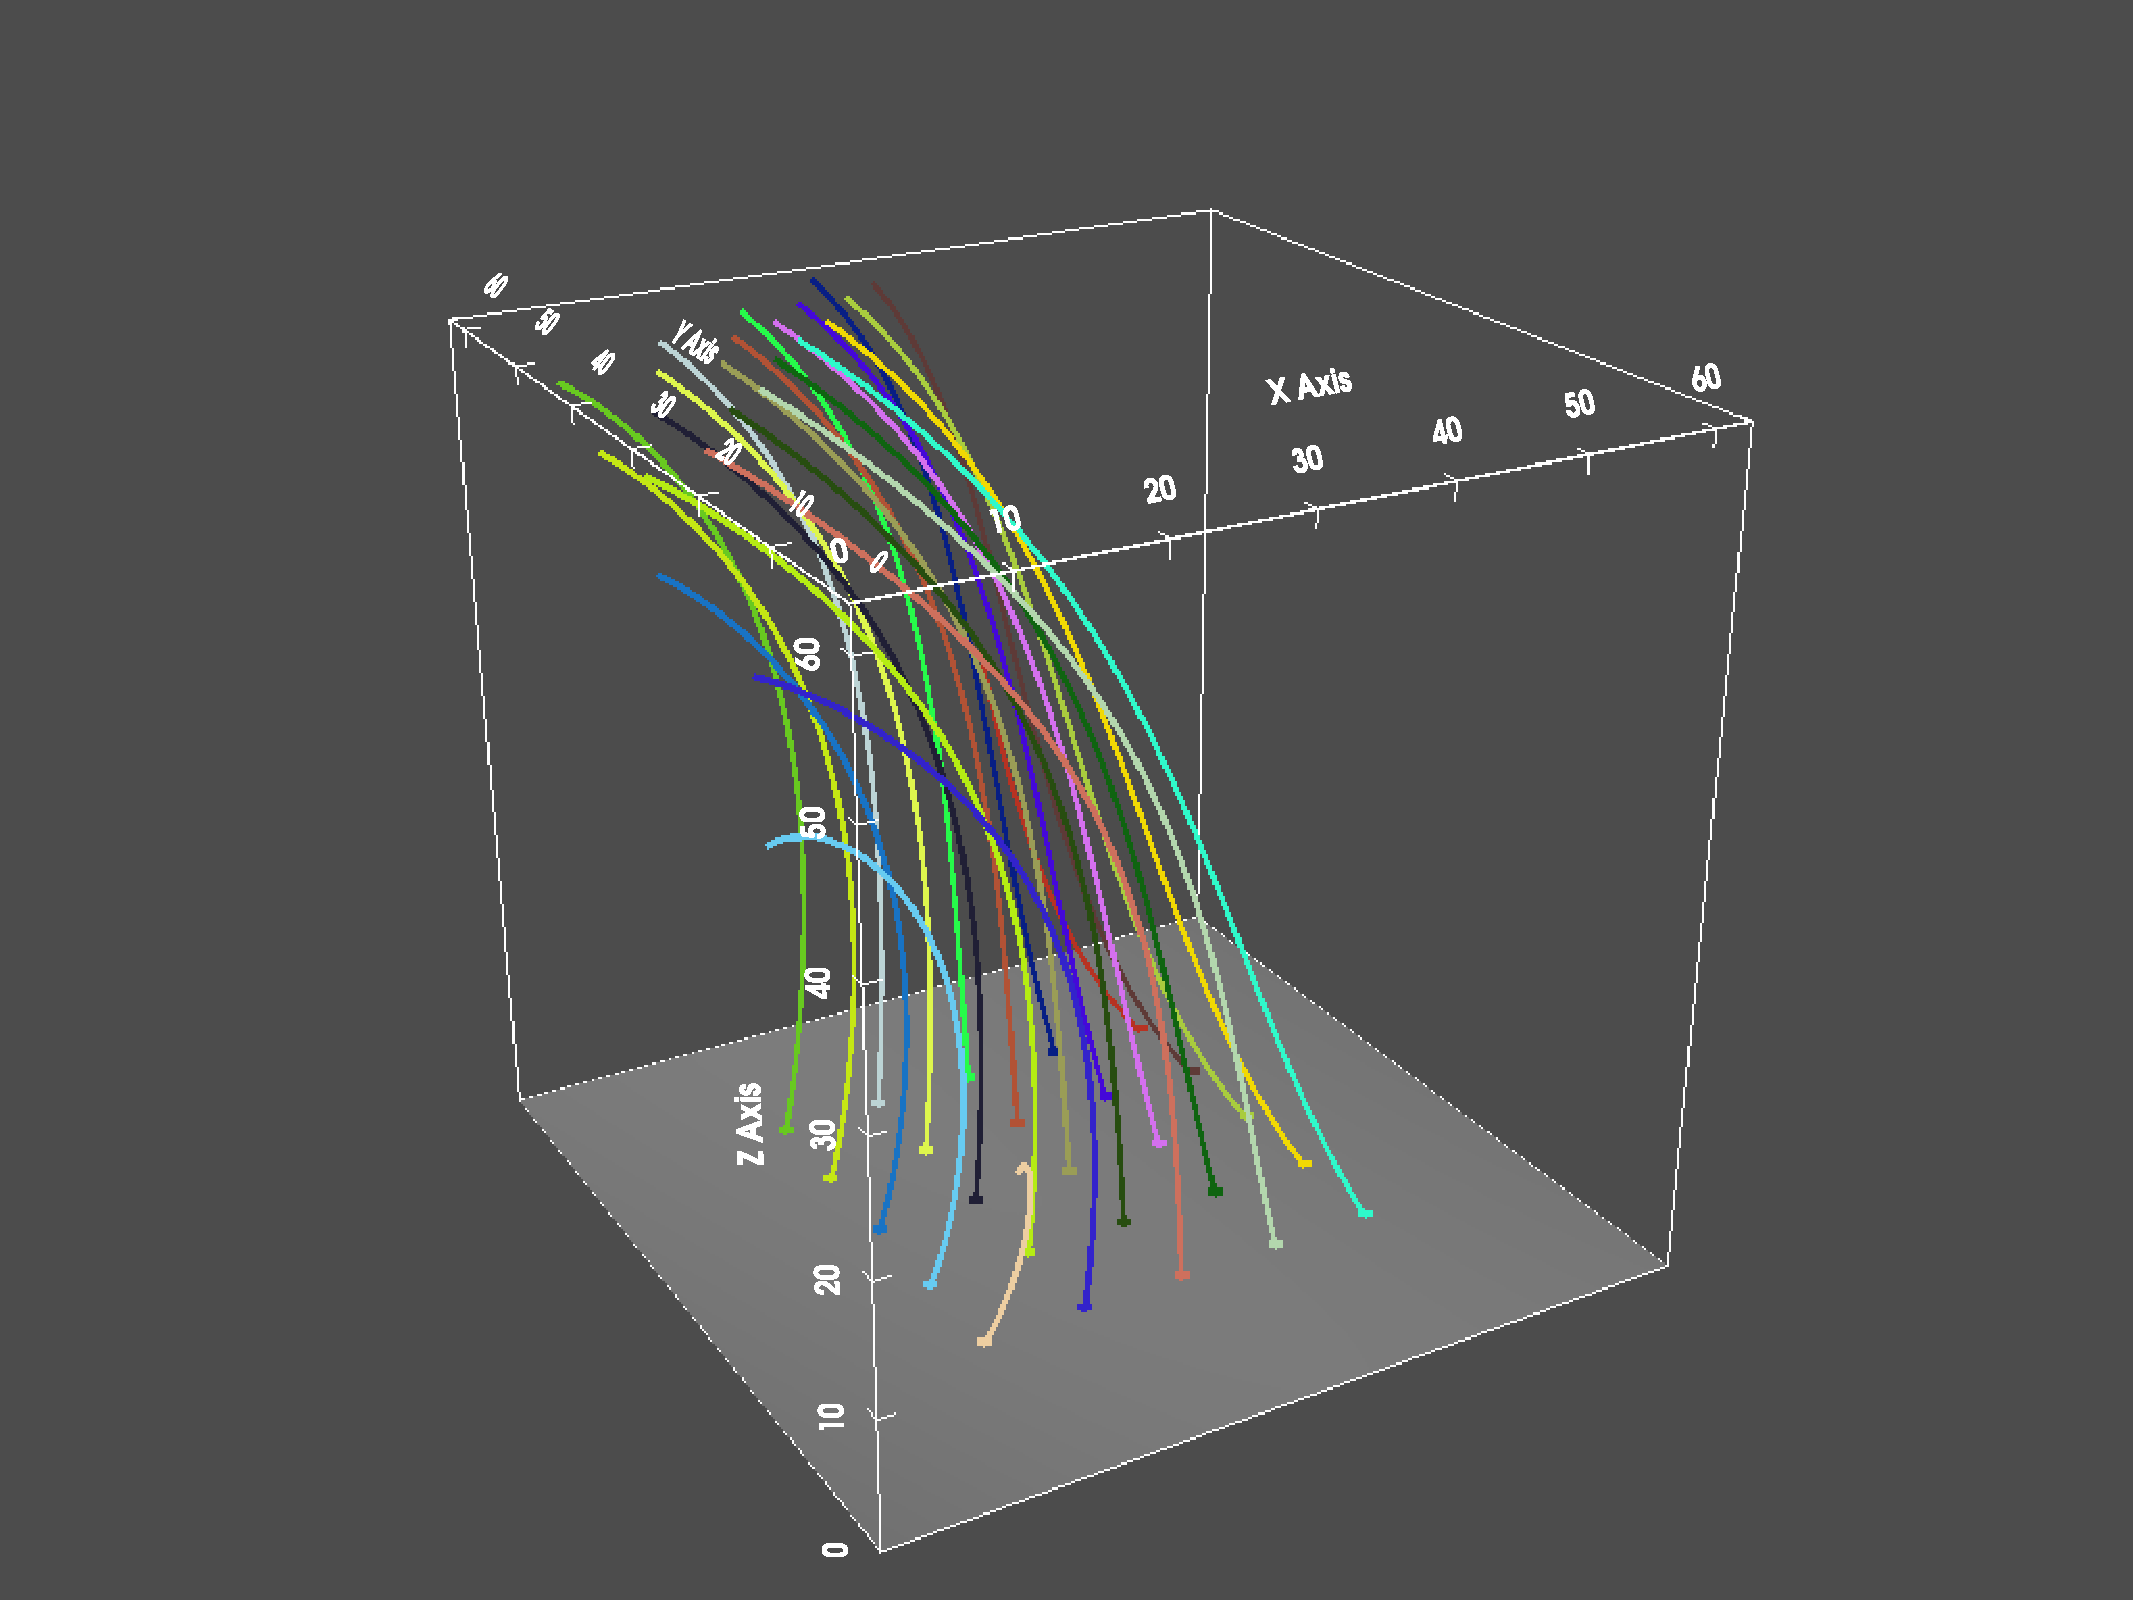
\includegraphics[trim={6cm 0cm 6cm 3cm}, clip, width=\linewidth]{"img/PINN_000100_xz_tilted.pdf"}
  \end{subfigure}

  \begin{subfigure}{.5\linewidth}
    \centering
    \caption{PINN(1000)}
    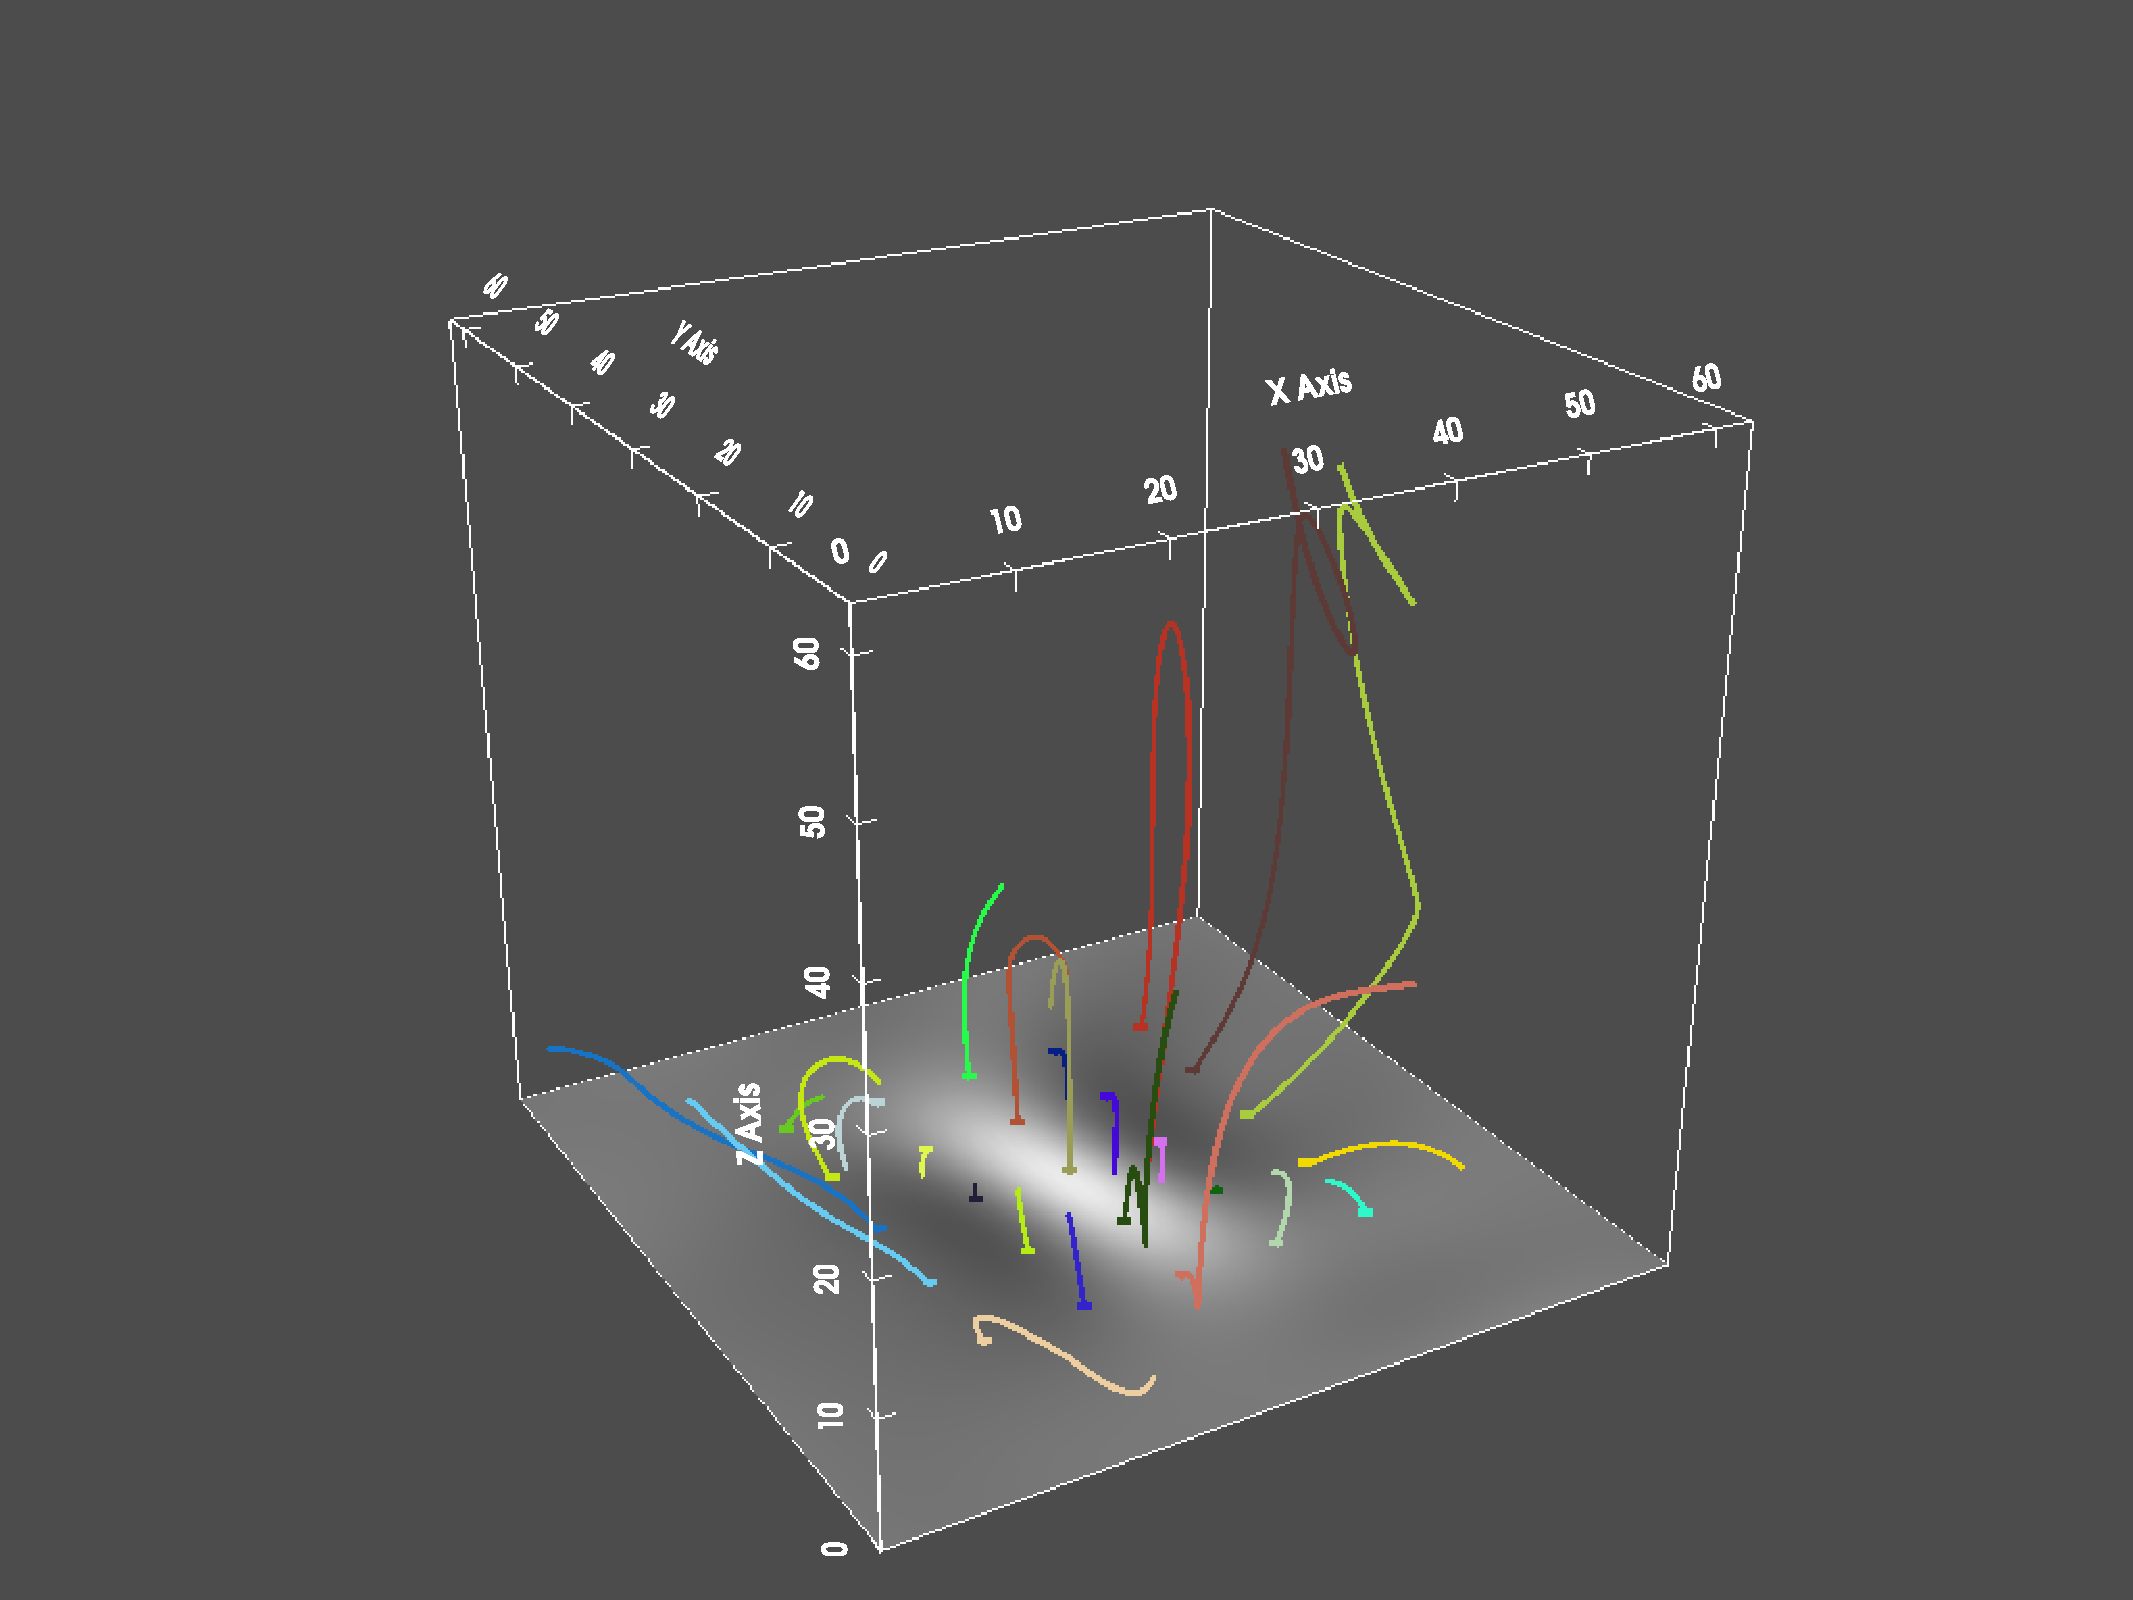
\includegraphics[trim={6cm 0cm 6cm 3cm}, clip, width=\linewidth]{"img/PINN_001000_xz_tilted.pdf"}
  \end{subfigure}%
  \begin{subfigure}{.5\linewidth}
    \centering
    \caption{PINN(10000)}
    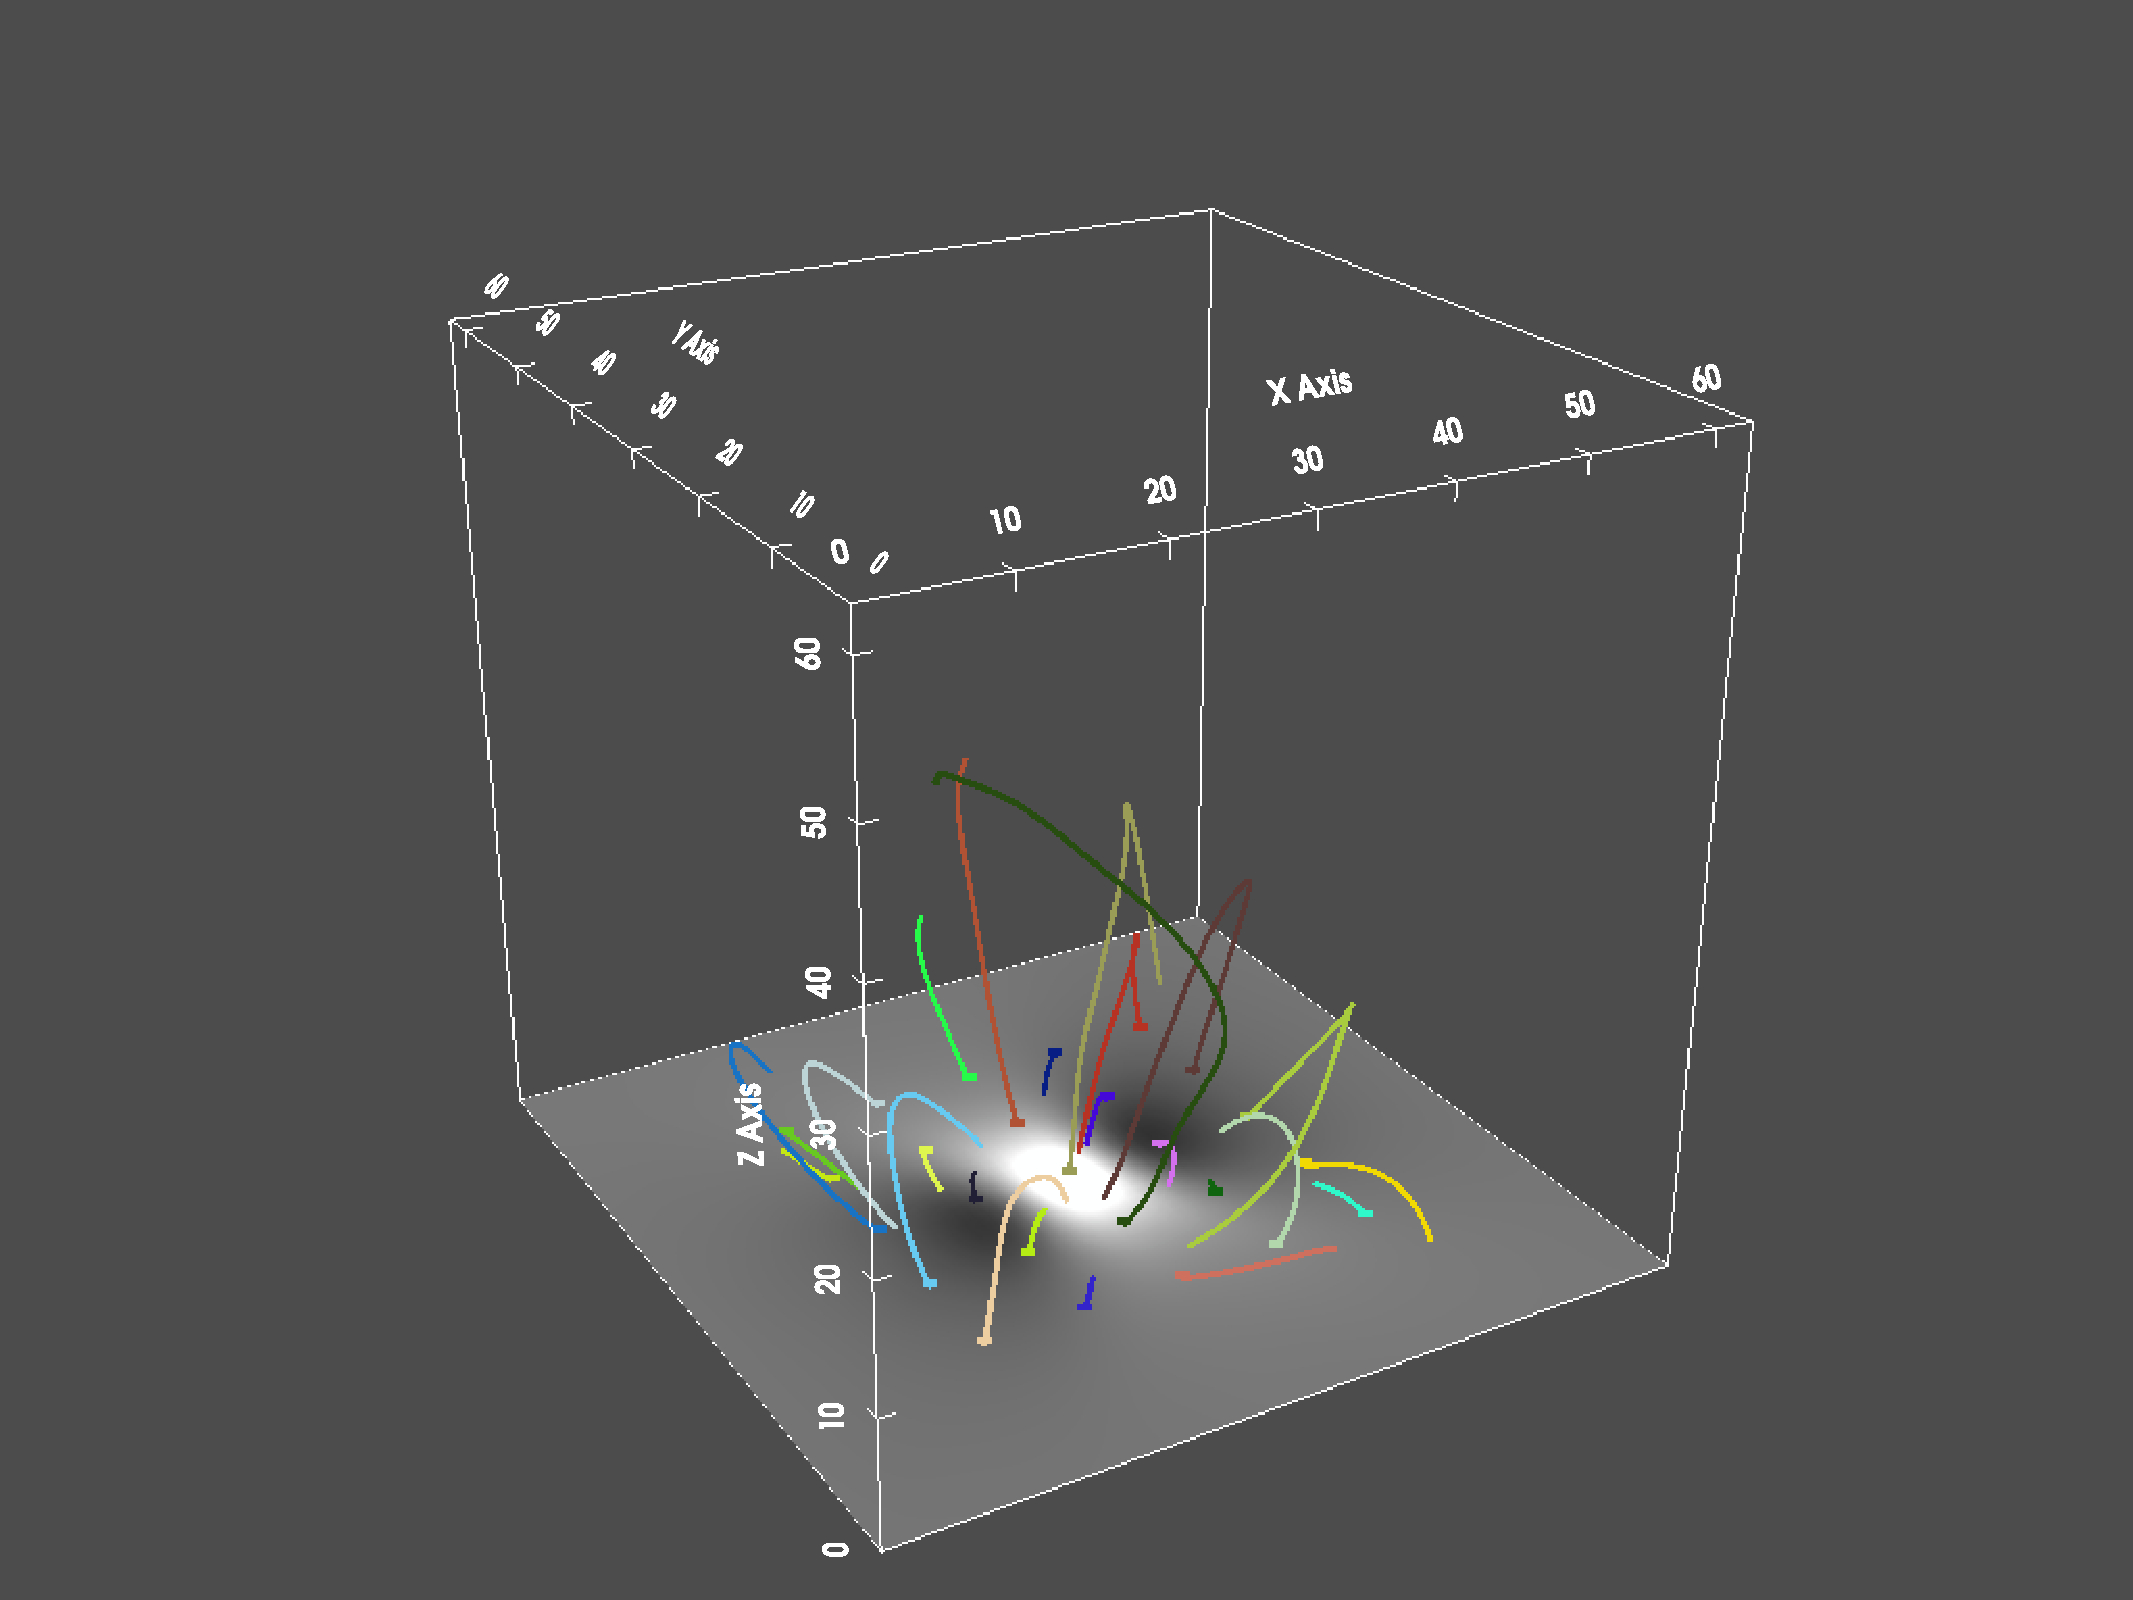
\includegraphics[trim={6cm 0cm 6cm 3cm}, clip, width=\linewidth]{"img/PINN_010000_xz_tilted.pdf"}
  \end{subfigure}

  \begin{subfigure}{.5\linewidth}
    \centering
    \caption{PINN(25000)}
    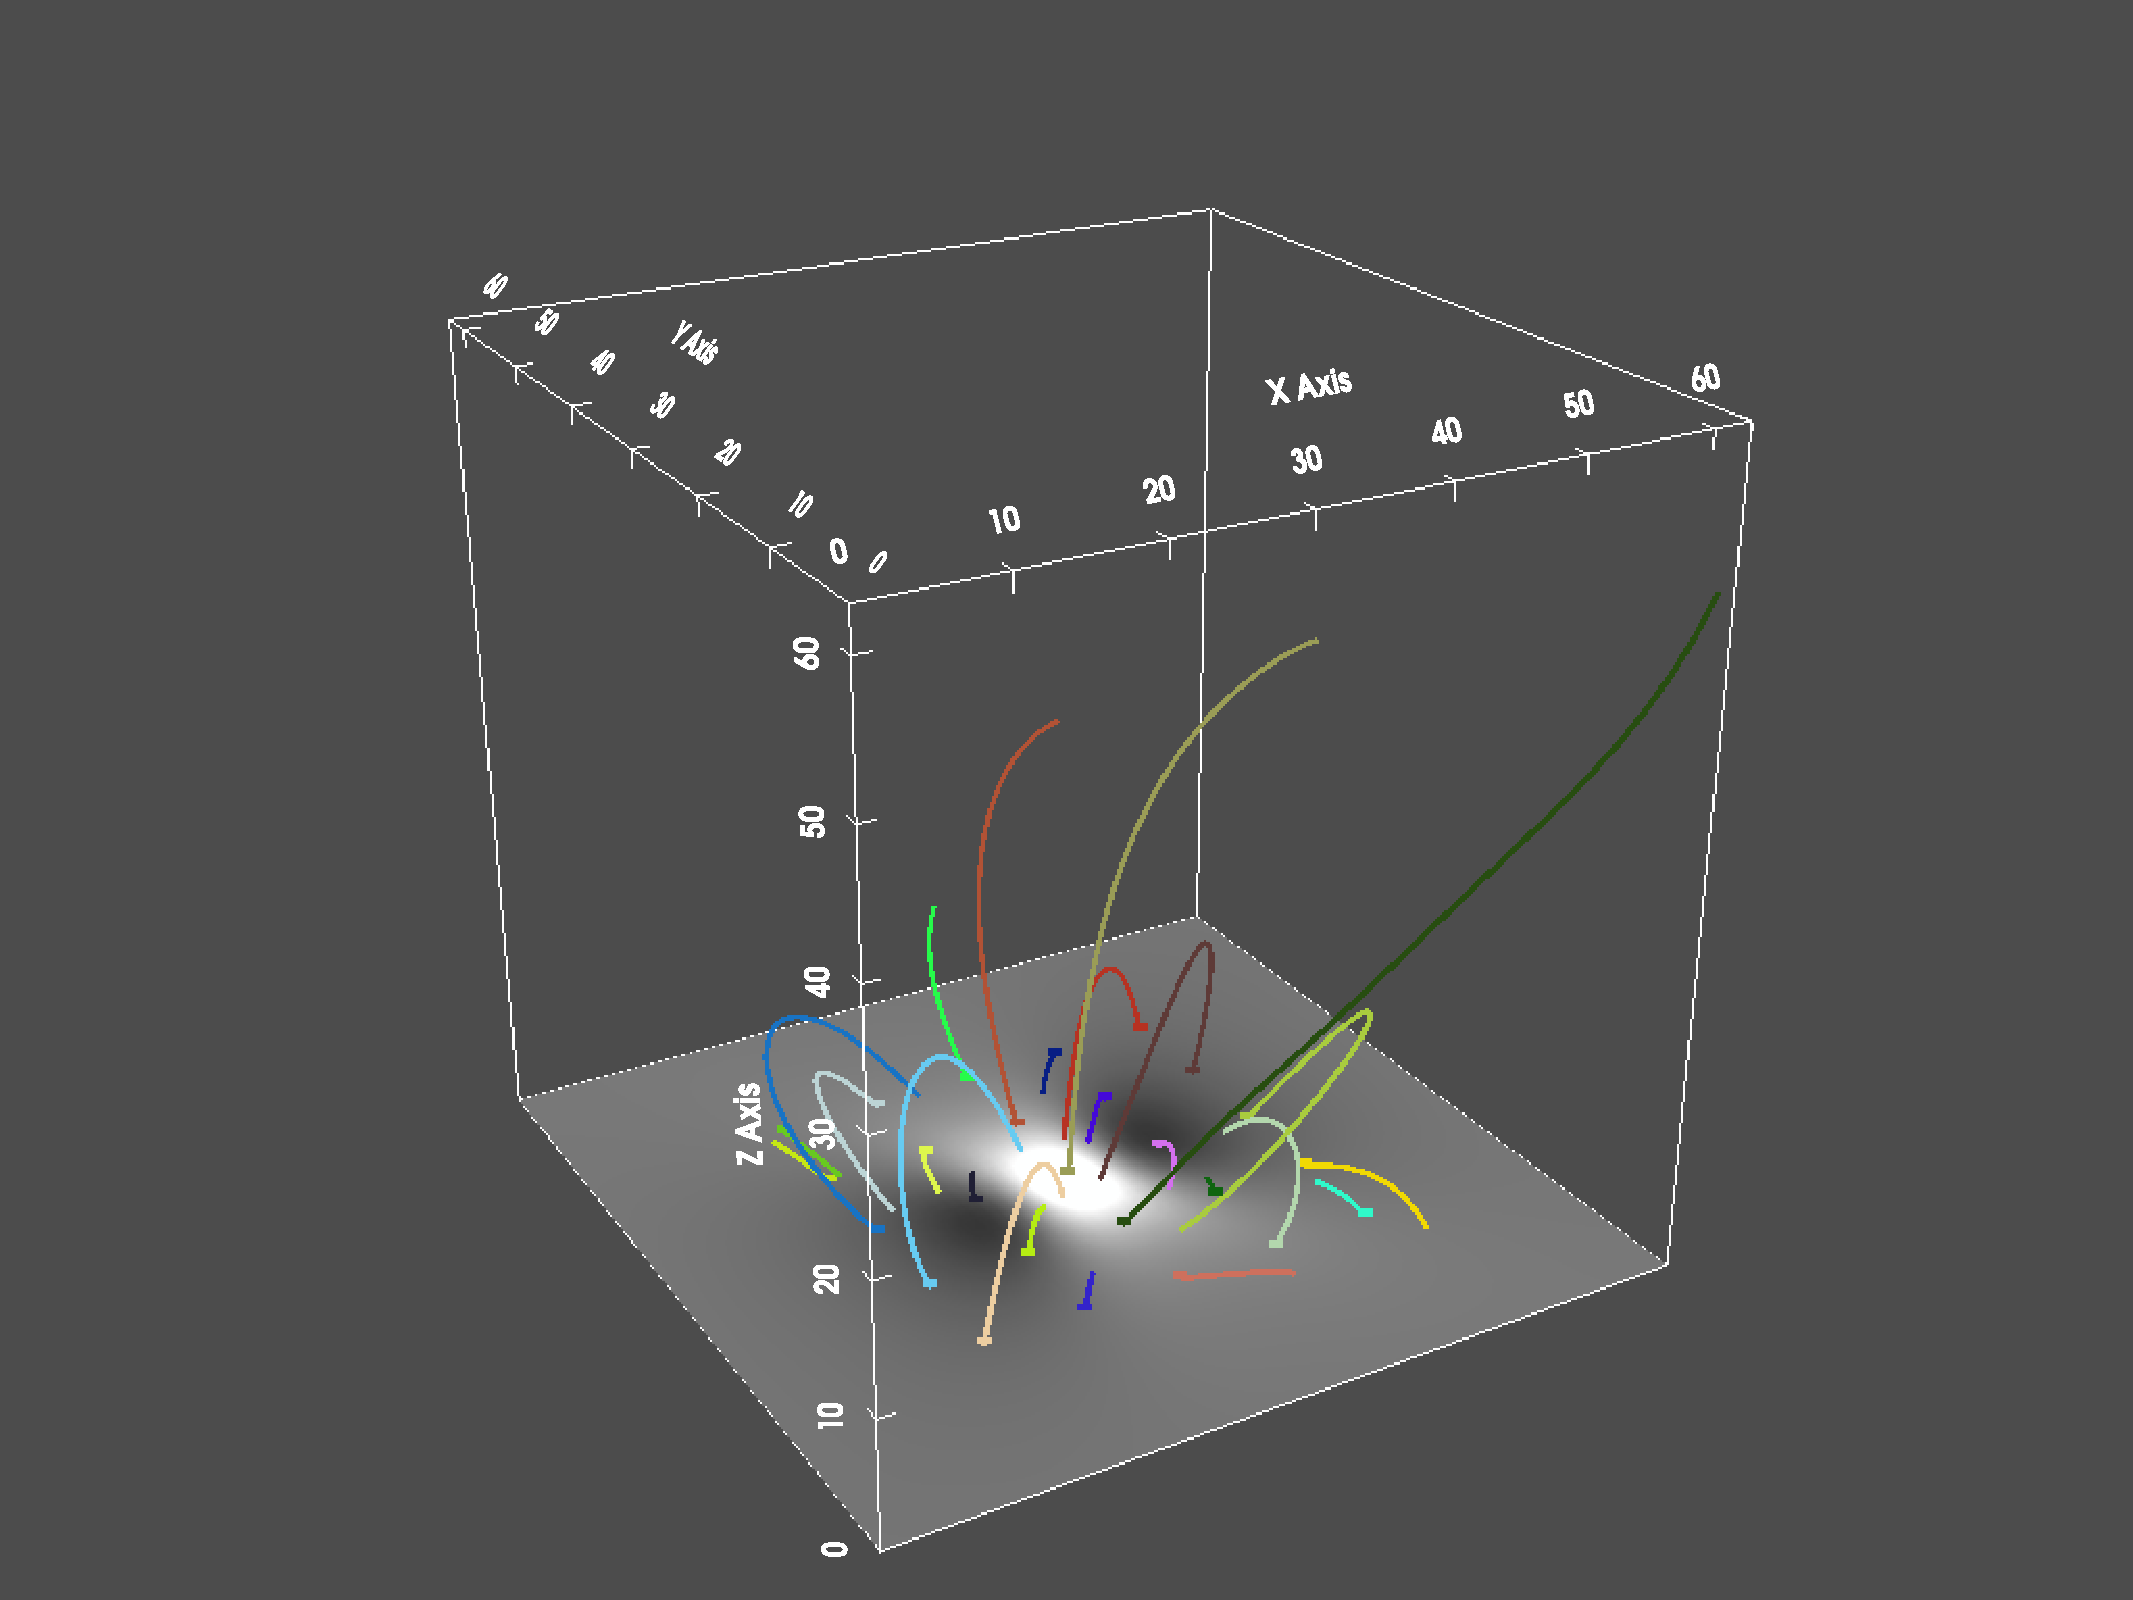
\includegraphics[trim={6cm 0cm 6cm 3cm}, clip, width=\linewidth]{"img/PINN_025000_xz_tilted.pdf"}
  \end{subfigure}%
  \begin{subfigure}{.5\linewidth}
    \centering
    \caption{PINN(50000)}
    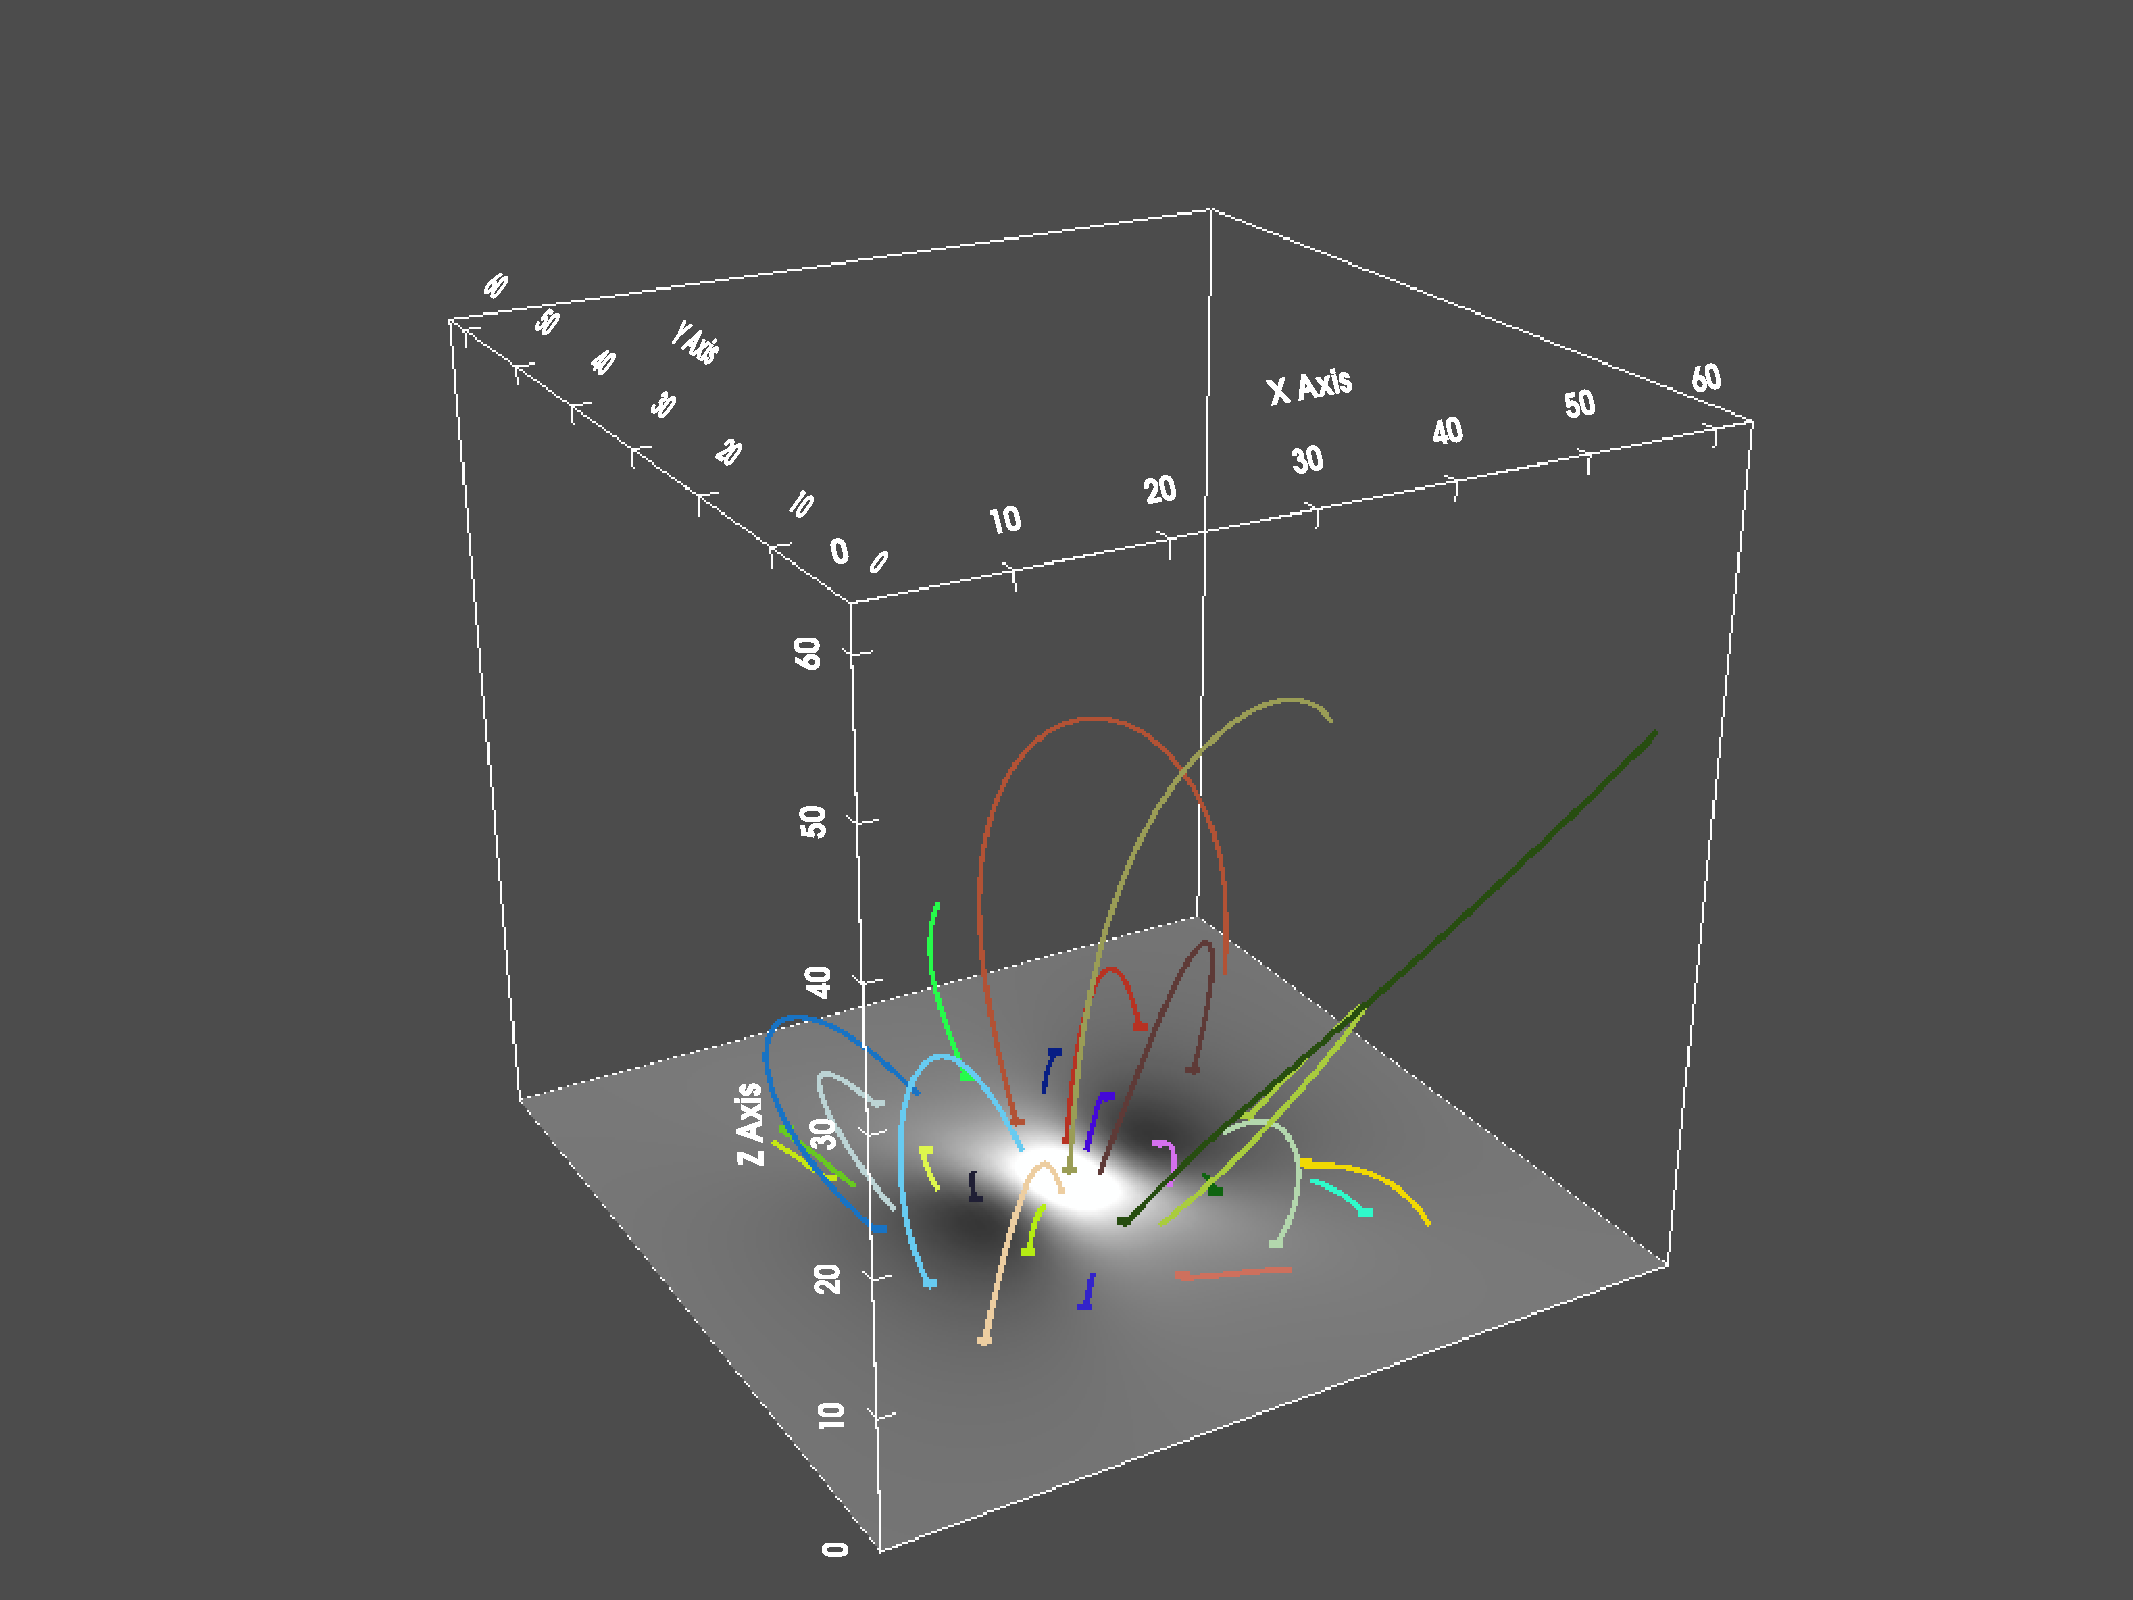
\includegraphics[trim={6cm 0cm 6cm 3cm}, clip, width=\linewidth]{"img/PINN_050000_xz_tilted.pdf"}
  \end{subfigure}
  
  \begin{subfigure}{.5\linewidth}
    \centering
    \caption{Potential}
    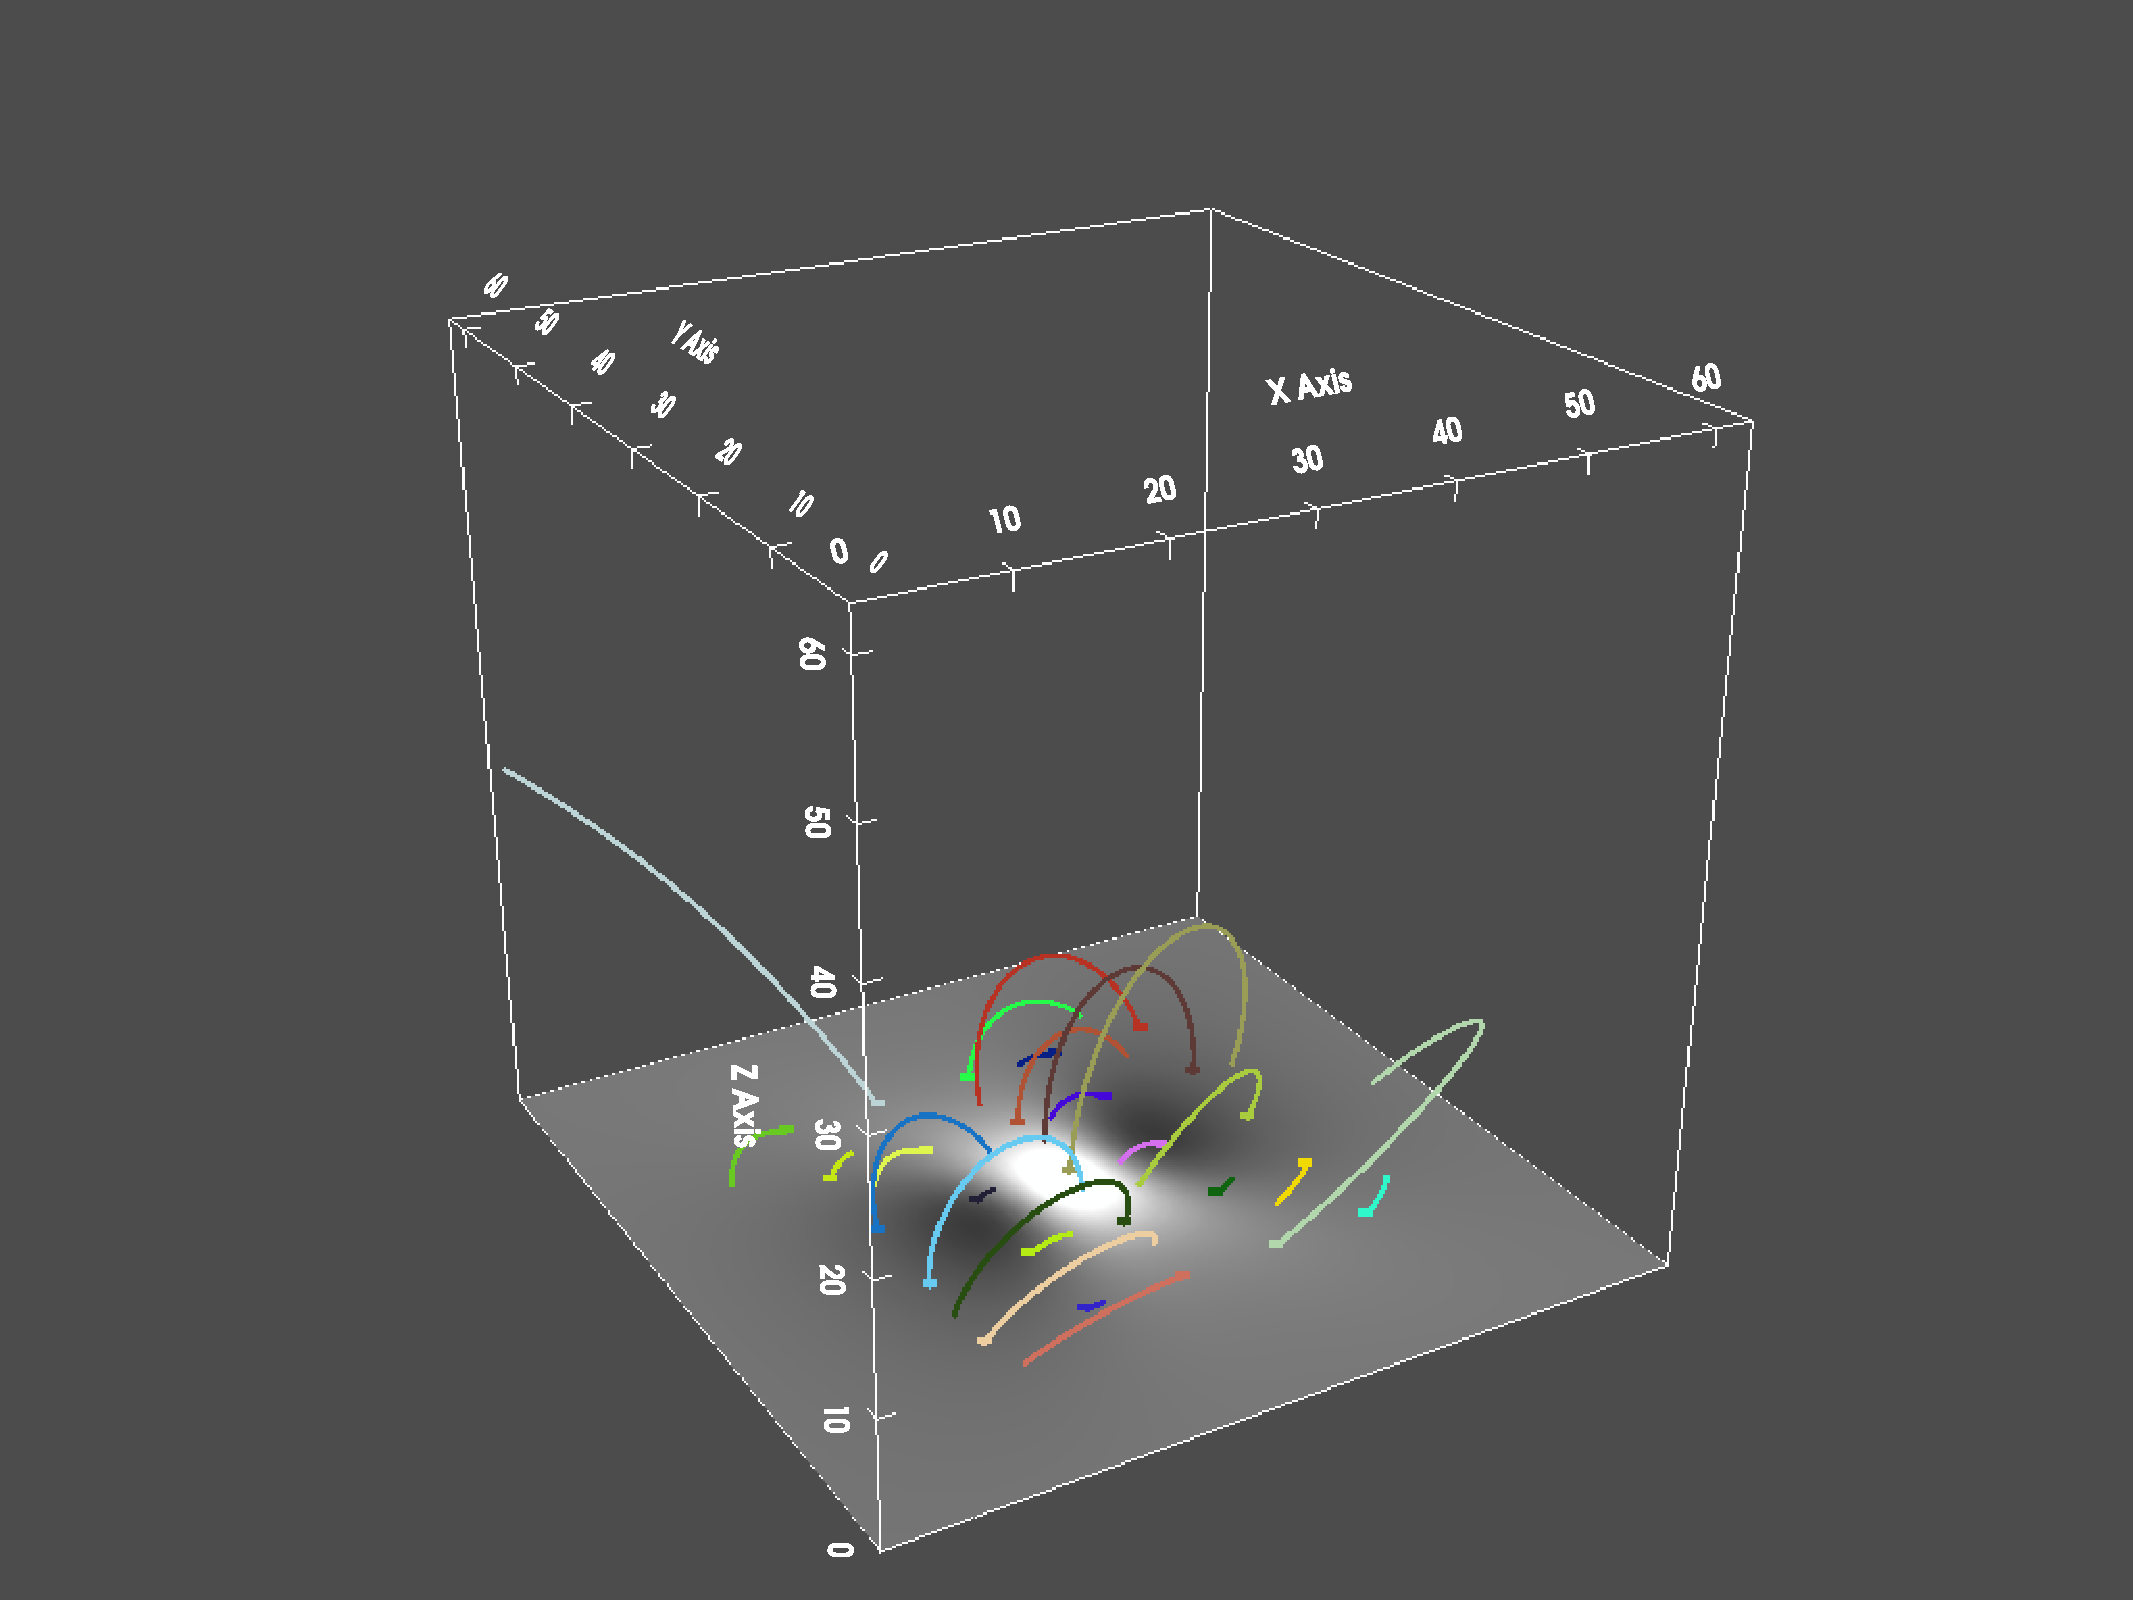
\includegraphics[trim={6cm 0cm 6cm 3cm}, clip, width=\linewidth]{"img/LL_pot_xz_tilted.pdf"}
  \end{subfigure}%
  \begin{subfigure}{.5\linewidth}
    \centering
    \caption{Low-Lou}
    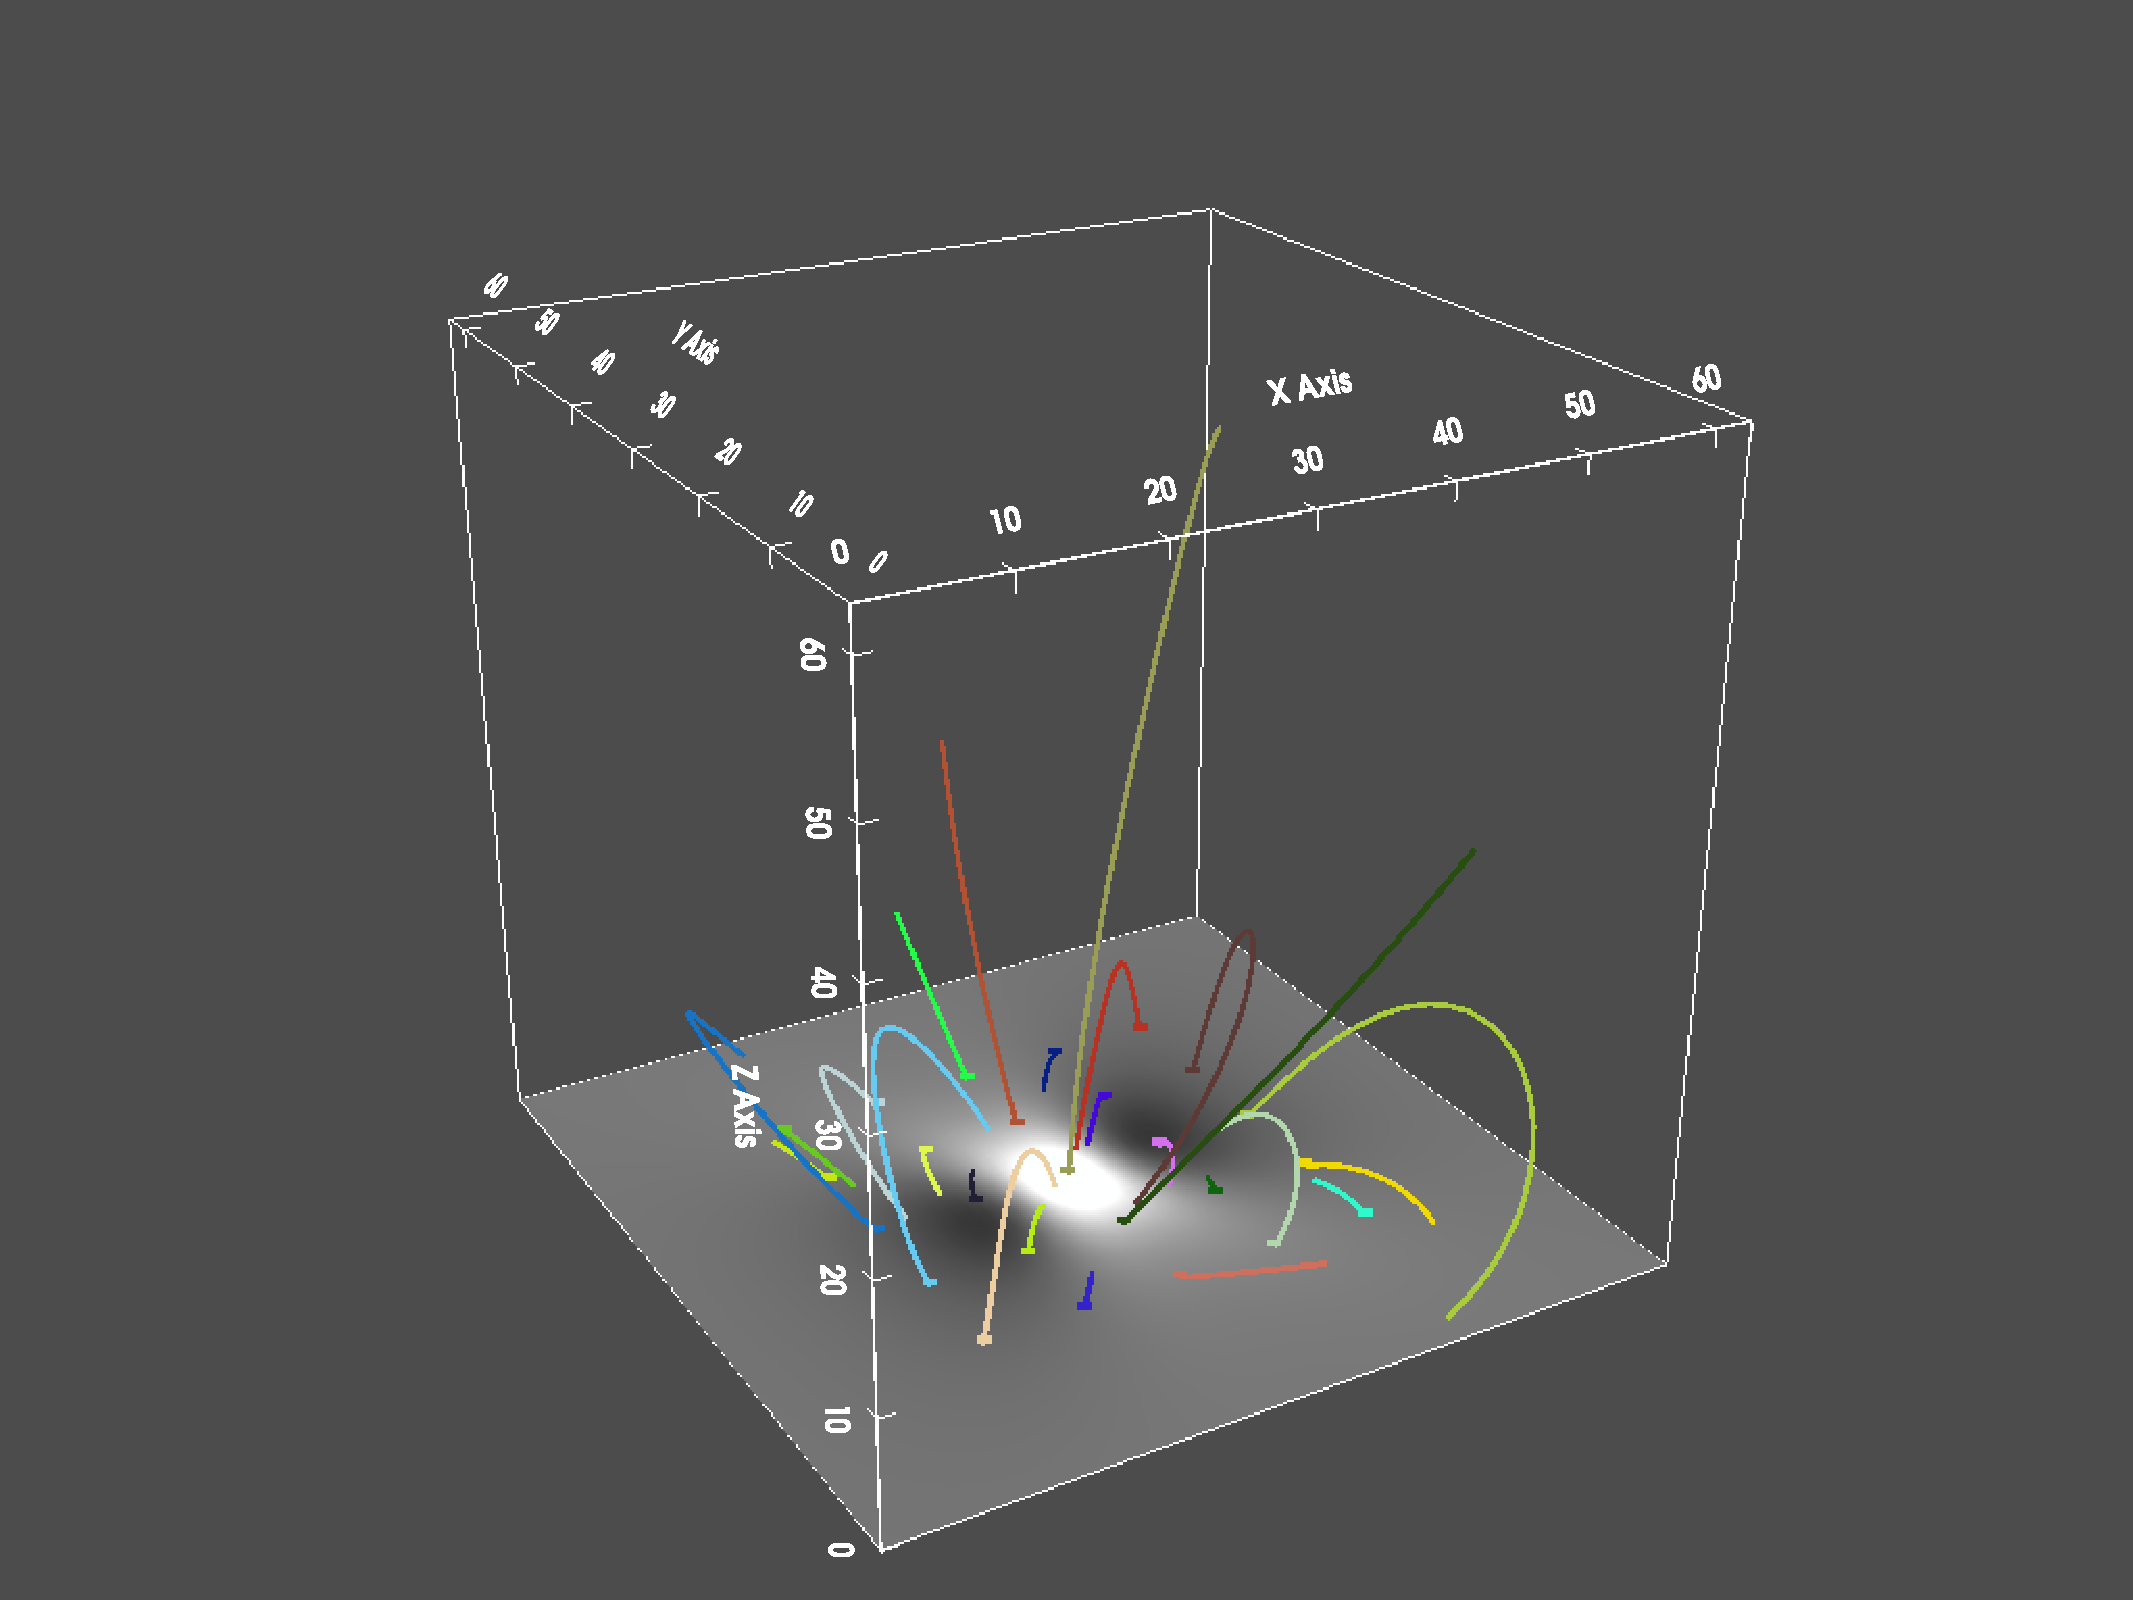
\includegraphics[trim={6cm 0cm 6cm 3cm}, clip, width=\linewidth]{"img/LL_xz_tilted.pdf"}
  \end{subfigure}
  
  \caption{The magnetic fields. Each field line is distinguished by its unique color, which is determined by its footpoint at $z=0$ plane.}\label{fig:xz_tilted}
\end{figure}

% \begin{figure}[h]
%   \centering
%   \includegraphics[width=\linewidth]{img/grafiek.png}
%   \caption{Graph of the function $sin(x) \cdot sin(y)$.
%     This figure is a bitmap, but of sufficiently high quality to be acceptable.
%     Take note of the legible axes and labels.
%   }\label{a}
% \end{figure}

% \lipsum[2-4]
% !TEX root = main.tex

\section{Conclusions}


The findings of this study yield valuable insights into the performance and capabilities of the physics-informed neural network method in calculating nonlinear force-free fields. The evaluation of various metrics demonstrates the PINN approach's ability to accurately reconstruct the Low-Lou model. The majority of these metrics demonstrate values that are quite similar with the analytical solutions, highlighting a substantial level of agreement between the PINN-reconstructed fields and the analytical solutions (\Cref{tab:metric} and \Cref{fig:metric}). Furthermore, this agreement is qualitatively confirmed by observing the graphical representation of the magnetic field (\Cref{fig:xy,fig:yz,fig:xz,fig:xz_tilted}). Additionally, the PINN approach successfully surpasses the potential field in terms of proximity to the Low-Lou solution, highlighting its effectiveness in capturing the complex magnetic field structures associated with solar activities.

While the PINN approach proves to be a promising method for calculating nonlinear force-free fields, this study also sheds light on its limitations. The figures of merit for the PINN(50000) model are inferior to those of the PINN(25000) model, despite the former having a lower loss value (\Cref{tab:metric}). This indicates the need for further exploration and refinement of loss functions. Additionally, the magnetic energy of the PINN(50000) model is lower than that of the analytical solution, suggesting that the PINN exhibits a spectral bias and struggles to learn high-frequency features. Enhancing the loss function and neural network architecture could improve the PINN's ability to capture high-frequency features and achieve even closer agreement with the analytical solutions. This research underscores the importance of ongoing efforts to enhance the performance and accuracy of the PINN approach, allowing for its wider application in solar physics and computational magnetohydrodynamics.

This thesis has presented a novel approach to calculating nonlinear force-free fields by employing physics-informed neural networks. This research specifically focuses on the application of physics-informed neural networks to the Low-Lou model, which provides semi-analytical solutions for nonlinear force-free fields. The results demonstrate the effectiveness of the proposed approach in accurately computing these fields. The successful implementation of physics-informed neural networks in this context highlights their versatility and potential for further advancements in the study of coronal magnetic fields and their relationship to solar phenomena. By recognizing the significance of coronal magnetic fields, this study demonstrates the potential of physics-informed neural networks in solar physics research.

\printbibliography


% \bibliographystyle{plainnat}
% \bibliography{literature}

\end{document}